\documentclass[11pt,a4paper]{article}

\newcommand{\titleinfo}{Using Analysts' Forecasts for Stock Predictions - An Entropic Tilting Approach}
\title{\titleinfo}
\def\authora{Christoph Frey}
\def\affiliation{Erasmus University Rotterdam} 
\def\email{\href{mailto:christoph.frey@gmail.com}{christoph.frey@gmail.com}}
\newcommand{\authorinfo}{\authora}

%%%%%%%%%%%%%%%%%%%%%%%%%%%
%%%        FONT         %%%
%%%%%%%%%%%%%%%%%%%%%%%%%%%
\usepackage[english]{babel}   			   % Language and hyphenation
\usepackage[OT1]{fontenc} 	               % PDF output as accents
\usepackage[utf8]{inputenc}              % directly input of accents
%\usepackage{garamondx}

%%%%%%%%%%%%%%%%%%%%%%%%%%%
%%%     PAGE STYLE      %%%
%%%%%%%%%%%%%%%%%%%%%%%%%%%
\usepackage[left=3cm, right=3cm, top=3cm, bottom=3cm]{geometry} % page layout
\usepackage{setspace} % line space
\usepackage{microtype}
%\setstretch{1.5}
%\pagestyle{empty}
%\setlength{\parindent}{0.5cm}
\doublespacing
%\setlength{\parskip}{0.2cm}

%%%%%%%%%%%%%%%%%%%%%%%%%%%
%%%    SECTION TITLES   %%%
%%%%%%%%%%%%%%%%%%%%%%%%%%%
\usepackage[medium]{titlesec}

%%%%%%%%%%%%%%%%%%%%%%%%%%%%%%%%%%%%%
%%% MATHEMATICS AND PROGRAMM CODE %%%
%%%%%%%%%%%%%%%%%%%%%%%%%%%%%%%%%%%%%
\usepackage{amsmath,amsfonts,amsthm}
\usepackage{marvosym,nicefrac}
%\usepackage{dsfont}
\usepackage{bm} % bold math symbolds
%\numberwithin{equation}{section} % equation numbers by section
\usepackage{listings} % code environment
\usepackage{stmaryrd}

\lstset{language=Matlab,
    	backgroundcolor={\color{lgrey}},
    	basicstyle={\footnotesize\ttfamily},
    	breakautoindent=true,
    	breakindent=10pt,
    	breaklines=true,
    	captionpos=t,
    	columns=fixed,
    	commentstyle={\itshape\color{colComments}},
    	extendedchars=true,
    	float=hbp,
    	frame=single,
    	identifierstyle={\color{colIdentifier}},
    	keywordstyle={\color{colKeys}},
    	numbers=right,
    	stepnumber=5,
    	firstnumber=1,
    	numberfirstline=true
    	%numbersep=1em,
    	numberstyle={\scriptsize\ttfamily},
    	showspaces=false,
    	showstringspaces=false,
    	stringstyle={\color{colString}},
    	tabsize=4,
    	xleftmargin=3px,
    	xrightmargin=3px
    	}

%%%%%%%%%%%%%%%%%%%%%%%%%%%
%%% GRAPHICS AND COLORS %%%
%%%%%%%%%%%%%%%%%%%%%%%%%%%
\usepackage{color,xcolor,graphicx}
\definecolor{DarkBlue}{rgb}{0.1,0,0.55}
\definecolor{DarkGreen}{RGB}{24,126,35}
% Colors for Matlab-Listings
\definecolor{lgrey}{RGB}{245,245,245}     % background
\definecolor{colKeys}{RGB}{0,0,255}       % blue
\definecolor{colIdentifier}{RGB}{0,0,0}	  % black
\definecolor{colComments}{RGB}{34,139,34} % green
\definecolor{colString}{RGB}{160,32,240}  % purple


%%%%%%%%%%%%%%%%%%%%%%%%%%
%%% LINKS AND HYPERREF %%%
%%%%%%%%%%%%%%%%%%%%%%%%%%
\usepackage[hyphens]{url}
\usepackage[pdfborder={0 0 0},bookmarks=true,breaklinks=true]{hyperref}
 \usepackage[anythingbreaks]{breakurl}
\hypersetup{colorlinks=true,
			citecolor = DarkBlue,
			pdftitle = {\titleinfo}, 
			pdfauthor = {\authorinfo},
			pdfpagelabels=TRUE,
			pdfstartview = {FitH},
			linkcolor = DarkBlue,
			urlcolor  = DarkBlue
			}




%%%%%%%%%%%%%%%%%%%%%%%%%%%%%%%%%%%%
%%% TABLES AND FIGURES AND LISTS %%%
%%%%%%%%%%%%%%%%%%%%%%%%%%%%%%%%%%%%
\usepackage{caption}
\usepackage{booktabs}
\usepackage{multirow,multicol}
\usepackage{longtable, tabularx, array, pbox, rotating,fullpage}
\usepackage{enumitem} % \begin{enumerate}[resume] to continue a previous list
%\usepackage{float}

%%%%%%%%%%%%%%%%%%%%%%%%%%%
%%%    VARIOUS STUFF    %%%
%%%%%%%%%%%%%%%%%%%%%%%%%%%
\usepackage{todonotes} 				   % To Do Lists with \todo{text}
\RequirePackage[l2tabu, orthodox]{nag} % Check for the 12 Tabus


%%%%%%%%%%%%%%%%%%%%
%%% BIBLIOGRAPHY %%%
%%%%%%%%%%%%%%%%%%%%
%\usepackage{harvard}
\usepackage[sectionbib]{natbib}
\let\natbibcitet\citet
\renewcommand\citet{\bibpunct{(}{)}{,}{a}{,}{,}\natbibcitet}
\let\natbibcitep\citep
\renewcommand\citep{\bibpunct{(}{)}{;}{a}{,}{;}\natbibcitep}

%%%%%%%%%%%%%%%%%%%%
%%% RandNotizen  %%%
%%%%%%%%%%%%%%%%%%%%
\setlength{\marginparwidth}{15mm}




%%%%%%%%%%%%%%%%%%%%%%%
%%% Special Content %%%
%%%%%%%%%%%%%%%%%%%%%%%
\newtheoremstyle{standard}% name
  {0,5cm}      % Space above
  {0,5cm}      % Space below
  {\upshape} % Body font
  {}         % Indent amount (empty = no indent, \parindent = para indent)
  {\bfseries}% Thm head font
  {}        % Punctuation after thm head
  {\newline} % Space after thm head: " " = normal interword space;
             % \newline = linebreak
  {}         % Thm head spec (can be left empty, meaning `normal')
%
\theoremstyle{standard}
\newtheorem{lem}{Lemma}[section]
\newtheorem{defi}{Definition}[section]
\newtheorem{theo}{Theorem}[section]
\newtheorem{prop}{Proposition}[section]
\newtheorem{assu}{Assumption}[section]
\newtheorem{excu}{Excursus}[section]
\newtheorem{prf}{Proof}[section]
%
%
\newtheoremstyle{notes}% name
  {0.5cm}      % Space above
  {0.5cm}      % Space below
  {} % Body font
  {}         % Indent amount (empty = no indent, \parindent = para indent)
  {\itshape}% Thm head font
  {}        % Punctuation after thm head
  {\newline} % Space after thm head: " " = normal interword space;
             % \newline = linebreak
  {}         % Thm head spec (can be left empty, meaning `normal')
%
\theoremstyle{notes}
\newtheorem{exam}{Example}[section]
\newtheorem{nota}{Notation}[section]
\newtheorem{rema}{Remark}[section]
\newtheorem{hypo}{Hypothesis}
\newtheorem{exerc}{\large{Exercise}}[subsection]
\newtheorem{exerc1}{\large{Exercise}}[section]

% Enumerate Counter
\newcounter{saveenumi}
\newcommand{\seti}{\setcounter{saveenumi}{\value{enumi}}}
\newcommand{\conti}{\setcounter{enumi}{\value{saveenumi}}}
% New Envirmoments
%\newcommand{\argmin}{\arg\!\min}
%\newcommand{\argmax}{\arg\!\max}

\newcommand{\am}[1]{\underset{#1}{\rm arg \, min } \,}
% arg min über {}
\newcommand{\amx}[1]{\underset{#1}{\rm arg max } \,}
% arg max über {}

% argmin, argmax
\newcommand{\argmin}[1]{\underset{#1}{\rm arg \, min } \,}
\newcommand{\argmax}[1]{\underset{#1}{\rm arg max } \,}


% Frieder's commands
%\newcommand{\N}[2]{\text{N} \left( \, #1 \, , \, #2 \, \right)}
\newcommand{\No}[1]{\text{N}\hspace{-0.05cm}\left(#1\right)}
\newcommand{\Ex}[1]{\text{E}\hspace{-0.05cm}\left(#1\right)}
\newcommand{\cov}[1]{\text{cov}\hspace{-0.05cm}\left(#1\right)}

%\newcommand{\IG}[2]{\text{IG} \left( \, #1 \, , \, #2 \, \right)}
\newcommand{\IG}[2]{\text{IG} \left( \, #1 \, , \, #2 \, \right)}


% Ingmar's commands
\DeclareMathOperator*{\pr}{Pr}
\newcommand{\p}[1]{\pr \left[ #1 \right]}
\newcommand{\pc}[2]{\pr \left[ #1 \left| #2 \right.\right]}
\newcommand{\pci}[3]{\pr_#3 \left[ #1 \left| #2 \right.\right]}
\DeclareMathOperator*{\Ew}{E}
\DeclareMathOperator*{\ewd}{\hat E}
\newcommand{\ew}{{\Ew}}
\newcommand{\e}[1]{\ensuremath{\Ew \left[ {#1} \right]}}
\newcommand{\edach}[1]{\ensuremath{\ewd \left[{#1} \right]}}
\newcommand{\ec}[2]{\Ew \left[ \left. #1 \right| #2 \right]}
\DeclareMathOperator*{\var}{V}
\newcommand{\va}[1]{\var\left[ {#1} \right]}
\newcommand{\vc}[2]{\var \left[ \left. #1 \right| #2 \right]}
\newcommand{\estvar}[1]{ \hat{\var} \left[ #1 \right]}
\DeclareMathOperator*{\cova}{Cov} \DeclareMathOperator*{\cor}{Corr}
%\newcommand{\cov}[1]{{\cova}\left[ {#1} \right]}
\newcommand{\corr}[1]{{\cor}\left[ {#1} \right]}
\newcommand{\no}[1]{{\rm N} \left( #1 \right)}
\newcommand{\nor}{\rm N}
\newcommand{\iidno}[1]{{\rm \stackrel{iid}{\sim} N} \left( #1 \right)}
\newcommand{\nv}[1]{\Phi \left( #1 \right)}
\DeclareMathOperator*{\median}{median} \DeclareMathOperator*{\mini}{min}
\DeclareMathOperator*{\maxi}{max}
\newcommand{\set}{\mathbb}
\newcommand{\setdef}[3]{\set #1 &:=& \left\{ #2 \quad : \quad #3 \right\}}
\newcommand{\plimn}{\underset{N\rightarrow \infty}{\rm plim } \quad }
\newcommand{\plimt}{\underset{T\rightarrow \infty}{\rm plim } \quad }
\newcommand{\plim}{\mathrm{p}\hspace*{-3pt}\lim\limits}
\newcommand{\pd}[2]{ \frac{\partial #1}{\partial #2}}


\newcommand{\Tab}[4]{
\begin{center}
$
\begin{array}{c}
\text{#1} \\
\text{ \parbox[t]{#4}{\vspace*{0,05cm}\footnotesize{\refstepcounter{table}{\bf Table \thetable: \hspace*{-0.25cm} #3}
#2}}}
\end{array}
$
\end{center}
}

\newcommand{\TabC}[4]{\addtocounter{table}{-1}
\begin{center}
$
\begin{array}{c}
\text{#1} \\
\text{ \parbox[t]{#4}{\vspace*{0,05cm}\footnotesize{\refstepcounter{table}{\bf Table \thetable~(cont'd): \hspace*{-0.25cm} #3}
#2}}}
\end{array}
$
\end{center}
}

\newcommand{\TabT}[5]{
\begin{center}
$
\begin{array}{l}
\text{#1} \\
\text{#2} \\
\text{ \parbox[t]{#5}{\vspace*{0,05cm}\footnotesize{\refstepcounter{table}{\bf Table \thetable: \hspace*{-0.25cm}#4}
#3}}}
\end{array}
$
\end{center}
}

\newcommand{\Fig}[4]{
\begin{center}
$
\begin{array}{l}
#1 \\
\text{ \parbox[t]{#4}{\vspace*{0,1cm}\footnotesize{\refstepcounter{figure}{\vspace*{-0.5cm} {\bf Figure \thefigure:} \hspace*{-0.15cm} #3} #2}}}
\end{array}
$
\end{center}
}

\newcommand{\FigC}[4]{\addtocounter{figure}{-1}
\begin{center}
$
\begin{array}{l}
#1 \\
\text{ \parbox[t]{#4}{\vspace*{0,1cm}\footnotesize{\refstepcounter{figure}{\vspace*{-0.5cm} {\bf Figure \thefigure~(cont'd).} \hspace*{-0.15cm} #3} #2}}}
\end{array}
$
\end{center}
}



% % % New Commands?

\newcommand{\beq}{\begin{equation}}
\newcommand{\eeq}{\end{equation}}
\newcommand{\beqno}{\begin{equation*}}
\newcommand{\eeqno}{\end{equation*}}
\newcommand{\beqn}{\begin{eqnarray}}
\newcommand{\eeqn}{\end{eqnarray}}
\newcommand{\beqnn}{\begin{eqnarray*}}
\newcommand{\eeqnn}{\end{eqnarray*}}
\newcommand{\balgn}{\begin{align}}
\newcommand{\ealgn}{\end{align}}
\newcommand{\balgnn}{\begin{align*}}
\newcommand{\ealgnn}{\end{align*}}
%\newcommand{\si}{\sigma}
\newcommand{\nono}{\nonumber}
\newcommand{\mbb}{\mathbb}
\newcommand{\mca}{\mathcal}
\newcommand{\msc}{\mathscr}
\newcommand{\ben}{\begin{enumerate}}
\newcommand{\een}{\end{enumerate}}
\newcommand{\bit}{\begin{itemize}}
\newcommand{\eit}{\end{itemize}}
\newcommand{\lhs}{\hspace{0.4cm}}
\newcommand{\shs}{\hspace{0.2cm}}
\newcommand{\lvs}{\vspace{0.4cm}}
\newcommand{\svs}{\vspace{0.2cm}}
\newcommand{\mbbe}{\mathbb{E}}
\newcommand{\mbbv}{\mathbb{V}}
\newcommand{\mbbcv}{\mathbb{CV}}
\newcommand{\mc}{\multicolumn}
\newcommand{\bbm}{\begin{bmatrix}}
\newcommand{\ebm}{\end{bmatrix}}
\newcommand{\lf}{\lfloor}
\newcommand{\rf}{\rfloor}

\newcommand{\VEC}{\text{vec}}
%\newcommand{\E}{\text{E}}
\newcommand{\V}{\text{V}}

\newcommand{\hilit}[1]{ \textcolor{green}{\textbf{#1}}}


\begin{document}
\begin{titlepage}
\title{\titleinfo \thanks{I would like to thank Dick van Dijk and Winfried Pohlmeier for helpful comments.
Financial support by the German Science Foundation (DFG, Project ``Development and application of new methodologies of combining time series and expert survey data for economic forecasting.'') and the Graduate School of Decision Sciences (University of Konstanz) is gratefully acknowledged. All remaining errors are ours.}}
\author{\Large \authora\thanks{Econometric Institute, Erasmus School of Economics, Erasmus University Rotterdam, Room H11-32, P.O. Box 1738, NL-3000 DR Rotterdam, The Netherlands. Phone (office): (+31) 10 408 1253, fax: (+31) 10 4089162, email: \email.} \\[0.2cm] \large \affiliation}  


\date{{{\today}} \\}
\maketitle
\thispagestyle{empty}

\begin{abstract}
\noindent In this paper, we combine predictive density forecasts for US stock returns from Bayesian vector autoregressions with financial analysts' forecasts via entropic tilting. In particular, we modify the predictive density of the asset returns to match moment conditions that are formed based on average analysts' forecasts. The advantage of this approach is that we can combine model-based time-series information with external, forward-looking information in a parsimonious way using closed-form solutions. Using a model with time-varying coefficients and stochastic volatility, we show that tilting the predictive asset return distribution towards the mean and variance of target price implied expected returns  increase prediction accuracy for both point and density forecasts. %This also translates into portfolio gains for an investor who maximizes her expected utility.
\end{abstract}
\vfill
\noindent \textbf{Keywords:} Bayesian vector autoregression, return prediction, tilting\\
\textbf{JEL classification:} C11, C58, G11
\end{titlepage}

\begin{center}
{\LARGE \title{\titleinfo}}
\end{center}

\begin{abstract}
	\noindent In this paper, we combine predictive density forecasts for US stock returns from Bayesian vector autoregressions with financial analysts' forecasts via entropic tilting. In particular, we modify the predictive density of the asset returns to match moment conditions that are formed based on average analysts' forecasts. The advantage of this approach is that we can combine model-based time-series information with external, forward-looking information in a parsimonious way using closed-form solutions. Using a model with time-varying coefficients and stochastic volatility, we show that tilting the predictive asset return distribution towards the mean and variance of target price implied expected returns  increase prediction accuracy for both point and density forecasts.
\end{abstract}
\thispagestyle{empty}
\newpage

\section{Introduction}
\label{sec:intro}
%The recent financial crisis has revealed that the quantitative tools of portfolio and risk management were poorly understood not only by practitioners but also by the academic world and have failed to work in times where they were needed most. While theoretically founded portfolio strategies generally fail to outperform completely non-theoretical approaches as the equally weighted portfolio in terms of a wide range of common performance measures \citep{demiguel2009}, it is also true that estimation, model and parameter uncertainty can alter the optimal asset allocation and therefore the the optimal trade-off between the return and risk of the investment substantially \citep{avramov2010,brandt2010}.\\
%
\indent Predicting stock returns is a popular exercise for professionals and academics in finance. It is a challenging task because of estimation and model uncertainty, because of a substantial unpredictable component (shocks) in future stock returns and because successful forecasting models may be exploited by other market participants causing trading behavior that destroys the prediction power of the model. Recent empirical findings suggest that the equity premium is predictable when accounting for model and estimation uncertainty through time-varying parameters, stochastic volatility and by using Bayesian predictive regressions \citep{zellner1965,barberis2000,pettenuzzo2016}. While the amount of predictability from variables such as the dividend-earnings ratio is limited in terms of out-of-sample R$^2$, it can translate into substantial portfolio gains for an expected utility investor \citep{johannes2014}.\footnote{See \cite{rapach2013} for a recent overview on return predictability.}\\
%
\indent Most prediction models relate the future stock returns to past observations of asset specific variables such as the dividend yield or to general macroeconomic indicators such as inflation. However, the market stock price is forward-looking as it reflects the expectations of market participants about the future cash flows of the company. It is natural to expect that using forward-looking information should also be beneficial for stock return predictions. A recent example is \cite{metaxoglou2016}, who improve equity premium forecasts by using option prices. In this paper, we use professional analyst's forecasts to improve asset return predictions. We do so by reweighting the predictive return distributions by a method called \textit{entropic (exponential) tilting} to incorporate the information contained in analysts' forecasts, such as target prices. The idea of this method is to modify the predictive density of the asset returns to match certain moment conditions that are formed based on average analysts' forecasts. The advantage of this approach is that we can combine model-based time-series information with external, forward-looking information in a parsimonious way using closed-form solutions.\\
%
\indent Professional security analysts provide market analyses, make earnings forecasts and give investment advise by providing twelve months forward target prices and stock recommendations. Their reports and opinions can have major short- and long-run impact on stock prices \citep[e.g.][]{irvine2003} and provide a powerful way to disseminate financial information to market participants.\footnote{The US Bureaus of Labor statistics report over 275,000 thousand financial analysts jobs in 2014 (see \url{http://www.bls.gov/ooh/business-and-financial/financial-analysts.htm}, checked on 19.08.2015).} And a vast literature exists about the shortcomings of analyst forecasts revealing skewed incentives (conflicts of interest), herding and biases to please clients that may create market inefficiencies.\footnote{See  \cite{ramnath2008} for an in-depth review of the analyst forecast literature.}\\
%
\indent In this study, we do not evaluate the accuracy of the analysts' forecasts, but we use the (dis-)agreement in the analysts' forecast to regularize the predictive return distribution. In particular, we restrict the mean and variance of the predictive distribution to coincide with the mean and the variance of monthly target price implied expected returns, i.e. simple returns between the current spot and the target price. While we find that restricting the variance of the asset returns is beneficial in terms of out-of-sample performance, as it provides a forward looking measure for (un-)certainty in the market, only restricting the mean has no particular forecasting power. Target prices are usually higher than current spot prices and so there is an upward bias in the target price implied expected returns which is not beneficial for the forecast performance.\\
%
\indent Of course we could also include the analyst information simply as another predictor variable in the predictive regressions, but this would add further parameters and more estimation noise to the prediction problem. Using the analyst information instead in a tilting framework, we only change the shape of the predictive distribution by reweighting it and hence do not require the data to formalize the relationship between asset returns and target prices.\\
%
\indent Another econometric contribution of this paper is the use of a large Bayesian vector autoregressive system to formalize the predictive relationship between asset returns and a great number of predictor variables. To overcome the computational burden that arises in a recursive forecasting exercise, we adopt the so-called \textit{forgetting factors} approach of \cite{koop2013} which allows for all the features recently found to be important to find significant return predictability: Time-varying parameters, stochastic volatility, parameter shrinkage as well as dynamic model averaging and variable selection. The idea of forgetting factors is to approximate the conditional error term variance in a Kalman filter type estimation of the time-varying model, reducing the computational burden significantly. While \cite{dangl2012} used a similar forgetting factor approach for return prediction, we will combine this method with a Minnesota-type prior that restricts the parameter matrix to deal with the case of many predictors.\\
%
\indent It is also worth mentioning that market excess returns, such as the S\&P500, might not be the ideal candidate to find predictability, because of their aggregation over many sectors and industries. In this paper instead, we will investigate the predictability of individual assets by looking at a cross-section of Dow Jones index constituents. We will investigate if these returns are predictable using company-specific characteristics like the book-to-market ratio or by using market and economic indicators such as inflation. Out-of-sample studies for cross-sectional returns are limited and a few exceptions among others are \cite{avramov2002} and \cite{rapach2015}. While these studies use factor and industry portfolio returns, we fill the gap and go down to the level of individual equity asset predictability.\\    
%
%\indent Including many predictors in the prediction model increases its dimensionality and requires some sort of regularization. Here, we will rely on two of such  techniques. We will model a Bayesian vector autoregressive system for the predictive relationship between asset returns and the predictor variables. We allow for time-varying coefficients and stochastic volatility using shrinkage priors and model averaging techniques in the fashion of \cite{koop2013}. The idea of this approach is to use so-called \textit{forgetting factors} to approximate the conditional error term variance in a Kalman filter type estimation of the time-varying model, reducing the computational burden significantly. While \cite{dangl2012} used a similar forgetting factor approach for return prediction, we will combine this method with a Minnesota-type prior that restricts the parameter matrix to deal with the case of many predictors.\\
%
%\indent In a second step, we will reweight the predictive return distributions through a method called \textit{entropic (exponential) tilting} to incorporate external knowledge from analyst recommendations. The idea of this method is to modify the predictive density of the asset returns to match certain moment conditions that are formed based on average analysts' forecasts, for example target prices. The advantage of this approach is that we can combine model-based time-series information with external, forward-looking information in a parsimonious way using closed-form solutions. We will restrict the mean and variance of the predictive distribution to coincide with the mean and the variance of monthly target price implied expected returns, i.e. simple returns between the spot and the target price at each point $t$ divided by twelve. While we find that restricting the variance of the asset returns is beneficial in terms of out-of-sample performance, as it provides a forward looking measure for (un-)certainty in the market, only restricting the mean has no particular forecasting power. Since target prices are usually higher than current spot prices, there is an upward bias in the target price implied expected returns which reduces forecast performance.\\ 
%
 %This is very useful for high-dimensional systems. 
%
%\indent The paper is organized as follows. Section \ref{sec:literature} first summarizes the literature about the usefulness of analysts' forecasts and further motivates the use of traget prices as  and then provides an overview on the state of the art of return predictability for aggregated market indices as well as for cross-sections. Section \ref{sec:methodology} introduces the concept of entropic tilting and describes the applied Bayesian panel vector autoregression setting. Section \ref{sec:application} summarizes the set-up of the empirical study and presents the results. Section \ref{sec:conclusions} concludes and gives an outlook on further generalizations.
%
%\subsection{Sell-side financial information}
%Professional security analysts provide market analyses, make earnings forecasts and give investment advise by providing target prices and stock recommendations. Their reports and opinions can have major short- and long-run impact on stock prices \citep[e.g.][]{irvine2003} and provide a powerful way to disseminate financial information to market participants.\footnote{The US Bureaus of Labor statistics report over 275,000 thousand financial analysts jobs in 2014 (see \url{http://www.bls.gov/ooh/business-and-financial/financial-analysts.htm}, checked on 19.08.2015).} There exists a huge literature about the shortcomings of analyst forecasts revealing skewed incentives (conflicts of interest), herding and biases to please clients that may create %more asymmetric information 
%market inefficiencies.\footnote{See  \cite{ramnath2008} for an in-depth review of the analyst forecast literature.} A  great amount of the research either focuses on the accuracy of accounting related figures such as earnings forecasts %\citep{bradshaw2012a} 
%or on the impact of their publication on market prices to analyze the behavior and expectations of market participants.\\ 
%%A prominent example is \cite{bradshaw2012a} who investigate the predictive accuracy of analyst earnings forecasts against a random walk model and find that analysts' provide more precise forecast only for short horizons and for relative large firms. %For small and young firms and for longer horizons the random walk model dominates. 
%%Studies evaluating the investment value of analysts forecasts often only consider strategies that are based on sentiments on these forecasts, i.e. portfolios having long positions in stocks with favorable forecasts and short positions in stocks with unfavorables ones.\\
%%
%\indent In this study, we will use analysts' recommendations and target prices as predictors for the asset returns and we will use them to provide a signal (moment condition) about the predictive return distribution. %After that, we will form portfolios for a utility maximizing investor using the tilted joint predictive distribution of the asset returns. 
%Analyst recommendations are discrete signals (e.g., strong buy, buy, hold, sell, strong sell) about the current market value of a stock and target prices forecast the stock price over the next twelve months. The two seem to be, besides of various shortcomings mentioned for example by \cite[][p. 1935]{brav2003}% and contrary to earning forecasts that are typically made for a limited period (e.g., a fiscal quarter) only
%, relevant candidates to provide useful investment signals regarding the current and future stock valuation. If this is not the case, does, after all, at least the timing matters, e.g. can recommendation revisions or expected target price returns reveal useful information about future stock returns?
%\indent Already a great number of studies document the investment value of sell-side analyst research: \cite{barber2001,green2006} report portfolio benefits and abnormal returns from simple trading strategies that go long in stocks with favorable analyst recommendations and short in stocks unfavorable ratings. \cite{jegadeesh2004} instead finds that predictive power of the level of consensus analyst recommendations various substantially across assets and proposes to use the changes or revisions in consensus analyst recommendations instead. \cite{jegadeesh2006} applies this to build portfolio strategies that are long (short) in stocks with positive (negative) recommendation revisions and that yield significant positive abnormal risk-adjusted returns against the market. \cite{cvitanic2006} further shows that such simple long-short portfolios can be outperformed by more complicated multi-period expected utility maximizing strategies that are estimated using consensus analysts recommendations. This is not the case for \cite{he2013}, who finds no significant portfolio returns from a \cite{black1992} strategy incorporating analyst recommendations for the Australian stock market.\\
%%
%\indent The evidence for return predictability from target prices is also mixed: While \cite{brav2003} document that target prices are generally informative about future stock prices and that there are substantial short-term market reactions in the stock price to target changes, \cite{bonini2010} find little evidence for target price accuracy using different metrics measuring the prediction error between the target price and the current, twelve month forward and in-between spot prices. This is in line with \cite{bradshaw2012b} who find an average target price premium over the spot price of 15 percent and who report that only two thirds of the target prices are met by the stock price at some time during the forecast horizon in their sample. \cite{lin2016} instead considers changes in target prices, but also find no evidence that institutional trading activity alongside the direction of the target price revisions yields higher risk-adjusted out-of-sample returns. Nevertheless, \cite{da2011} finds that aggregating stocks across sectors according to their the twelve month forward target price implied expected return, i.e. simple return between the current and the target price, yields significant risk-adjusted abnormal returns for different long-short portfolio.
% That is the old text.
%\cite{jegadeesh2004} also find predictive power in the level of consensus analyst recommendations, but it varies across stocks with favorable and unfavorable fundamental characteristics. Instead, the authors propose to use changes in consensus analyst recommendations and find that this yields a robust predictor variables with a positive significant impact on future stock returns. Further, \cite{jegadeesh2006} analyze the effect of recommendation revisions on stock returns for the G7 countries. The authors document significant price reaction on the day and the day after a recommendation change that also translate into an up- and downward stock price drifts in the long-run. Portfolio strategies that are long (short) in an equally weighted index of stocks with positive (negative) recommendation changes in the last 1, 3 or 6 months yield significant positive abnormal risk-adjusted returns against the market. The effects are most strongest in the US, where there is the greatest number of recommendations. \cite{brown2013} is another example to show the impact of analysts recommendation by analyzing the herding behavior of mutual funds. They find that downgrades in recommendations has a larger effect yielding a significant contemporaneous price effect followed by a sharp subsequent price reversal. %Such an overreaction to recommendation reversals can lead to price destabilizing with an increasing level of mutual fund ownership of stocks.  
%In a portfolio context, \cite{he2013} find that stocks with favorable (unfavorable) recommendations yield higher (lower) risk-adjusted return than the in the Australian stock market, using a portfolio strategy with daily rebalancing based on a \cite{black1992} approach to incorporate analyst recommendations does not produce out-of-sample risk-adjusted excess returns after transaction costs that are significantly higher than the market return. %to determine long (short) positions in stocks with favorable (unfavorable) recommendations
%In contrast to this, \cite{cvitanic2006} show that a simple long-short portfolios can be outperformed by more complicated expected utility maximizing strategies. In a multi-period dynamic rebalancing portfolio framework, the authors explore an inter-temporal CAPM that allows for abnormal returns (alpha). The authors derive the optimal strategy for an expected power-utility maximizing investor and estimate the securities alpha using average analysts recommendations. While their optimized strategy outperforms simple long-short allocations, the results are stronger for long horizons and for securities with a greater number of recommendations.
%
%\indent The evidence for return predictability from target prices is also mixed: Generally, \cite{brav2003} document that (i) target prices are informative about the future stock prices, both unconditionally and conditional on contemporaneously issued recommendation and earnings forecast revisions, (ii) that there are substantial short-term market reactions in the stock price to target changes and (iii) that on average, target prices are generally higher than current spot prices (about 30 percent). In contrast to this, \cite{bonini2010} find little evidence for target price accuracy using different metrics measuring the prediction error between current and future (twelve months ahead) spot price, and between target price and the maximum/minimum stock price in between. %The authors also find a negative correlation between the prediction accuracy in target prices and the analysts intensity of research and the market momentum indicating a systematical bias in the analysts forecasts. 
%This is in line with \cite{bradshaw2012b} who find only weak forecast performance in target prices and report an average target price premium over the spot price of  15\%. In there sample, only two thirds of the target prices are met by the stock price at some time during the forecast horizon. This happen less often for high volatility stocks, but more often during time periods of firm-specific positive price momentum and overall large positive market returns.  Most recently, \cite{lin2016} considers changes in target prices and analyzes the institutional trading of a large set of US firms. While they document increased institutional trading activity alongside the direction of the target price revisions, they find no statistical significant evidence that this trading yields higher risk-adjusted out-of-sample returns. \cite{da2011} answer this by arguing that aggregating stocks across sectors according to their the twelve month forward target price implied expected return, i.e. simple return between the current and the target price, yields significant positive portfolio effects. They sort S\&P500 stocks in this way within different industry sectors into nine groups and then form equally weighted portfolios of each group across sectors. Taking a long position in the portfolio with the highest expected target returns and a short position in the portfolio with the lowest expected target returns yields significant risk-adjusted monthly abnormal returns of over 200 basis points. %However, sorting all stocks across their expected target return across all industries at once renders the results to be insignificant.
%\begin{itemize}
%\item While testing the accuracy of analysts' earnings forecasts reveals their incentives, it is natural to use analyst recommendations and target prices for portfolio constructing.
%\item The efficient market hypothesis suggest that all information concerning a stock is already refelcted in its price.
%\item Financial researchers and practitioners have long been interested in understanding how the activities of financial analysts affect capital market efficiency.
%\item Equity analysis provides investors with information on the current and future prospects of listed companies. 
%\item \cite{rapach2015} use a mixed frequency time series model to outperform earnings forecasts from analysts despite their timing and information advantage.
%\end{itemize}
%\subsection{A promising example}
%Before heading to the main analysis, a motivating example is needed. 
\indent Figure \ref{fig:ibmpriceplot} serves as an illustrative example. It shows the IBM spot price, the mean twelve months forward target price and the percentage of buy recommendations from all recommendations (buy, sell, hold) of the IBM stock. While the correlation between the spot and the target price is almost perfect (0.9721), spot price and buy recommendations are negatively correlated (-0.6470). In the plot the target price is almost always higher than the current spot price, indicating an upward bias in these forecasts. The only times when the two plots coincide is after price drops when the spot price starts to increase again, i.e. in late 2002, 2007 and 2014. That is, financial analyst might not be able to predict trend changes (regime switches) but they are able to forecast the price direction. This is in line with the more volatile buy recommendations, which only on average indicate the stock price direction.\\% Intuitively, increasing prices  an high price should lead to fewer buy and more sell and hold recommendations.\\
%
\indent While this pattern is similar also for the other 19 stocks considered here, comparing the target price with the observed spot price twelve months ahead gives a mixed picture. Table \ref{tab:rmsfe} provides the root mean squared forecast errors (RMSFE) between the two for the 20 stocks and compares it to the two year historical mean. Only for 11 out of the 20 stocks the target prices were better forecasts than the historical mean, e.g. for the IBM stock.\\
%
\indent Figure \ref{fig:ibmclsdplot} gives an idea about the predictive power of individual predictors against a benchmark intercept only model by plotting three out-of-sample performance measures for the IBM stock. Considering the first panel showing the cumulative sum of squared forecast errors differentials, we see that mostly all predictors fail to outperform the intercept only model, especially in the financial crisis. The only exception is the log return of the mean analyst twelve months forward target prices.  Note that values above zero indicate that a given predictor has better forecast performance than the benchmark model, while negative values suggest the opposite. The target price itself only has some predictive power between 2008 and 2010 (square markers). This might suggest that not the level of the predicted target price matters, but that the timing of the shifts, represented by the target price implied returns, have predictive power. Also, we see that the average analyst recommendations have no particular predictive power for the IBM stock.\\  
%
\indent The paper is now organized as follows. Section \ref{sec:literature} gives an overview about the findings from other authors trying to exploit analysts' forecasts and reviews the state of the art on return predictability. Section \ref{sec:methodology} describes the applied Bayesian vector autoregression model, which relies on the forgetting factor approach by \cite{koop2013} for large systems. We then introduce the concept of entropic tilting and explain how we translate the analyst forecasts into moment conditions for the predictive return distribution. Section \ref{sec:application} summarizes the set-up of the empirical study and presents the results. Section \ref{sec:conclusions} concludes and gives an outlook on further generalizations.






	

\section{Predictive powers}
\label{sec:literature}
\subsection{Analysts' forecasts}
\indent A great number of studies document the investment value of sell-side analyst research: \cite{barber2001,green2006} report portfolio benefits and abnormal returns from simple trading strategies that go long in stocks with favorable analyst recommendations and short in stocks with unfavorable ratings. \cite{jegadeesh2004} instead finds that the predictive power of the level of consensus analyst recommendations varies substantially across assets and proposes to use the changes or revisions in consensus analyst recommendations instead. \cite{jegadeesh2006} applies this to build portfolio strategies that are long (short) in stocks with positive (negative) recommendation revisions yielding significant positive abnormal risk-adjusted returns against the market. \cite{cvitanic2006} further shows that such simple long-short portfolios can be outperformed by more complicated multi-period expected utility maximizing strategies that are estimated using consensus analysts recommendations. This is not the case for \cite{he2013}, who find no significant portfolio returns from a \cite{black1992} strategy incorporating analyst recommendations for the Australian stock market.\\
%
\indent The evidence for return predictability from target prices is even more mixed: While \cite{brav2003} show that target prices are generally informative about future stock prices and that there are substantial short-term market reactions in the stock price to target changes, \cite{bonini2010} find little evidence for target price accuracy using different metrics measuring the prediction error between the target price and the current, twelve months forward and in-between spot prices. This is in line with \cite{bradshaw2012b} who find an average target price premium over the spot price of 15 percent and who report that only two thirds of the target prices are met by the stock price at some time during the forecast horizon in their sample. \cite{lin2016} instead consider changes in target prices, but also find no evidence that institutional trading activity following the direction of the target price revisions yields higher risk-adjusted out-of-sample returns. Only \cite{da2011} find that aggregating stocks across sectors according to their twelve month forward target price implied expected return, i.e. simple return between the current and the target price, yields significant risk-adjusted abnormal returns for different long-short portfolio.\\
%
\indent However, despite this discouraging evidence, none of the studies above operate in a Bayesian framework using predictive distributions and none consider a tilting framework in which the analyst's forecasts serve as a shrinkage target instead of just being another predictor variable.  

\subsection{Predictive regressions}
\cite{kandel1987} propose a vector autoregression formulation to jointly model the dynamics of asset returns and its predictor:
\begin{align}
	\label{eqn:ks1987}
	r_{t+1}&=a_r+b_rx_t+\varepsilon_{r,t+1},\\
	x_{t+1}&=a_x+b_xx_t+\varepsilon_{x,t+1},\label{eqn:ks1987_2}
\end{align}
where $x_t$ is the explanatory variable (for example the dividend yield) and $r_t$ is the asset return and $\varepsilon_t=(\varepsilon_{r,t},\varepsilon_{x,t})'\stackrel{iid}{\sim}\No{0,\Sigma}$. Here, equation (\ref{eqn:ks1987_2}) is needed to model the times-series dynamics of the predictor variable trough an autoregressive process. This model has been used by various authors to investigate the predictability of the equity premium and to build portfolios using the predictive return distribution.\\ 
%
%\indent \cite{campbell1988} uses it to show that the market equity premium can be predicted by the dividend yield as the predictor variable. Since then, the literature has provided evidence and counter-evidence for return predictability.\\
%
\indent \cite{kandel1996} estimate the model using Bayesian priors that center the mean of the slope coefficient in (\ref{eqn:ks1987}) to zero, implying no predictability and a weak form of market efficiency. Using a one-period model with power utility, they find that not accounting for the variability in the regressor can decrease the annual certainty equivalent up to 3\%.\\
%
\indent \cite{pastor2000a} extends the model in (\ref{eqn:ks1987}) - (\ref{eqn:ks1987_2}) to a multivariate regression for $N$ risky assets and apply a Normal inverse Wishart prior for the model mean and variance of the asset returns. They interpret the prior as a form to describe the disbelief of the investor in the given prediction/asset-pricing model. Importantly, they find that the optimal portfolio weights tend to be less extreme when using the joint predictive distribution of the asset returns by integrating out the estimated model parameters.% $\mu$ and $\Sigma$. %Similarly, \cite{pastor2000b} find that the difference in the portfolio selection based on various asset models vanishes when the degree of belief about their correctness decreased. %Eventually, \citet{wachter2009} model the investors disbelief in predictability through an informative prior on the  $R^2$ of the predictive regression.
\\
%
\indent While these studies are concerned with investments for one period, \cite{barberis2000} investigates the impact of changes in the prediction variables to the asset allocation in the long-term. As the variance of the cumulative log returns grows less than linear in the investment horizon, stocks appear less risky and so an investor should allocate more funds to stocks when the investment horizon increases. However such an over-allocating to stocks disappears when accounting for estimation uncertainty and possible structural breaks in the parameters of the prediction model \citep{pettenuzzo2011}.\\
%
\indent Stock returns may be predicted by company specific characteristics such as the dividend-price ratio or they may be macroeconomic indicators. Given the great number of potential predictor variables, shrinkage and model averaging methods are natural candidates to reduce model risk in predictive regressions. For example, \citet{avramov2002} considers 14 predictor variables and extend the predictive system in (\ref{eqn:ks1987}) - (\ref{eqn:ks1987_2}). The author averages over all $2^{14}=16384$ distinct model to predict the asset returns by weighting each model by its posterior weight. Similar examples for Bayesian model averaging (BMA) in the literature include \citet{cremers2002} and \citet{wachter2015}. Furthermore, \citet{pettenuzzo2016} propose a Bayesian density combination approach over 15 predictor variables that, instead of minimizing a statistical loss function, maximizes the certainty equivalent of a power utility investor and report robust out-of-sample predictability across various performance measures.\\
%
\indent Studies using time-varying coefficients in prediction models have also become numerous in recent years: While \cite{welch2008} find no evidence for significant in-sample and out-of-sample predictability of 14 variables on the equity premium using a rolling window estimation, \cite{dangl2012} find predictability in one-step-ahead forecasts of monthly S\&P 500 returns by using Bayesian predictive regressions with time-varying parameters and model averaging over a range of predictor variables. Using time-varying coefficients as well as stochastic volatility but only two possible predictor variables, \cite{johannes2014} document statistically and economically significant portfolio benefits for a dynamic rebalancing power utility investor using Bayesian predictive regressions. Very recently, \cite{feng2016} propose to perform a \textit{predictive} cross-validation approach to select the right amount of shrinkage that provides optimal posterior point estimates instead of marginalizing out the model parameters to obtain a full predictive return distribution. \\
%
\indent Very related to this paper is \cite{metaxoglou2016}, who are the first to apply entropic tilting to predict the US equity premium. For this, the authors rely on option data to form corresponding  moment conditions. In particular, the authors use the second moment of the risk-neutral density implied by option prices on the S\&P500 to tilt predictive distributions obtained from OLS model combinations with individual predictors, where the combination weights are chosen such that the model minimizes a discounted mean squared forecast error \citep{rapach2013}. For monthly returns and one-step ahead forecasts, they find that the tilted forecasts outperform an historical average based on various performance measures and for various sub-samples.
%
%\subsection{US equity premium predictability}
%\cite{ang2007} find significant in-sample predictability of the dividend yield, the short-term interest rate and the earnings yield on the equity premium (measured by S\&P500 excess returns) only for short horizons and only when excluding the 1990ies. While the predictive power of the dividend yield increases when including the short-term rate, which could be explained by an omitted variable bias, the predictive power of the earnings yield is very similar to the dividend yield, indicating that mostly the denominator (the price of the asset) has predictive power.\\
%\indent Examples that focus on varying coefficients in asset prediction models are among many other \cite{lettau2008}, \cite{welch2008}, \cite{dangl2012}, and \cite{johannes2014}.\\
%%
%\indent \cite{welch2008} find no evidence for significant in-sample and out-of-sample predictability of 14 variables on the equity premium measured by the excess return of the S\&P500 index. Besides considering individual predictive regressions for every predictor, they also consider a model including all variables and a model performing subset selection based on a cumulative predictive error criterion in every period. While the model including everything delivers significant in-sample predictability, it can not outperform the historical average out-of-sample. The model selection approach only delivers good performance until 1976, a couple of years after the oil price. The authors stress the point that excluding post-crisis periods (such as 1973-1975) deteriorates the performance of the many of the predictor variables against the historical average even further. The results hold for longer and shorter forecast horizons as well as for sub-sample periods.\\
%%
%\indent \cite{dangl2012} find predictability in a Bayesian regression setting with time-varying coefficients, but no stochastic volatility, and a range of predictor variables for a one-step-ahead forecast horizon. They apply a Bayesian model averaging approach that outperforms single regressor predictions. In connection with the business cycle, they show that out-of-sample predictability is stronger in recessions than in expansions. This can be used for market timing in portfolio allocation.\\
%%
%\indent Further in an expected utility framework with dynamic portfolio rebalancing, \cite{johannes2014} investigate the portfolio performance from predictive regressions over time. They authors use a prediction model that incorporates payout yield-based expected return predictors with time-varying coefficients and stochastic volatility. They estimate the model sequentially through partical filters to simulate a Bayesian learning problem for the investor about the parameters. They find statistically and economically significant out-of-sample portfolio benefits for a power utility investor who uses such models and accounts for parameter uncertainty by using predictive return distributions ($p(r_{t+h}|r_t)$) of return predictability when forming optimal portfolios.\\
%%
%\indent Using the VAR return prediction model of \cite{kandel1996} given in equation (\ref{eqn:ks1996}), \cite{feng2016} use the duality of regularization penalties (such as a lasso prior) on the mean and variances of asset returns and prior distributions to propose a \textit{predictive} cross-validation approach to select the right amount of shrinkage. While they are finding the optimal posterior point predictions, their approach does not marginalize out the parameters to obtain a full predictive return distribution.\\
%%
%\indent \cite{pettenuzzo2016} propose a Bayesian density combination approach that maximizes the certainty equivalent of a power utility investor who chooses between the market index (S\&P500 returns) and the risk free investment. They consider 15 predictor variables in individual models with constant parameters and with time-varying parameters and stochastic volatility. They find robust out-of-sample predictability across performance measures and also test predictability for Fama/French industry portfolios.\\
%%
%\indent \cite{metaxoglou2016} are the first to apply entropic tilting to predict the US equity premium. For this, the authors rely on option data to form corresponding  moment conditions. In particular, the authors use the second moment of the risk-neutral density implied by option prices on the S\&P500 to tilt predictive distributions obtained from OLS model combinations with individual predictors.  The combination weights are chosen such that the model minimizes a discounted mean squared forecast error (DMSFE) \citep{rapach2013}. For monthly returns and one-step ahead forecasts, they find that the tilted forecasts outperform an historical  based on various performance measures and for various sub-samples.
%
%\subsection{Cross-sectional stock return predictability}
%
%Examples are \cite{avramov2002} and \cite{rapach2015}. For a detailed review the reader is guided to \citet[][Section 4.2., page 374]{rapach2013}.

% to old to be true
%The model can be written in matrix form for $k$ explanatory variables using some zero restrictions:
%\begin{equation}
%\label{eqn:ks1987matrix}
%\begin{pmatrix} y_2'\\ \vdots \\ y_T' \end{pmatrix} = \begin{pmatrix} 1 & x_1'\\ 1 & \vdots \\ 1 & x_{T-1}' \end{pmatrix}\,B+\begin{pmatrix} \varepsilon_2'\\ \vdots \\ \varepsilon_T' \end{pmatrix}\,\Longleftrightarrow\,Y=XB+E,
%\end{equation}
%where $Y$ is a matrix of dimension $(T-1)\times(k+1)$, $X$ of $(T-1)\times(k+1)$, $B$ of $(k+1)\times(k+1)$, and $E$ of $(T-1)\times(k+1)$. For all $t$ it holds that $\varepsilon_t=(\varepsilon_{r,t},\varepsilon_{x,t})'\stackrel{iid}{\sim}\N{0,\Sigma}$.\\
%%
%\indent The model in (\ref{eqn:ks1987}) as been used by various authors to investigate portfolio problems: \cite{kandel1996} use a Bayesian version of it and investiate the predictive power and portfolio gains from using the dividend yield as the predictor variable. The argument is that, although the typical coefficient of determination for each equation in the system is lower than 10\%, the impact of changes in the regressor variable can have a sizable impact on the optimal asset allocation. They use a one-period model with power utility and an informative prior specification that centers the mean of the slope coefficient to zero, which implies a weak form of market efficiency. They find that not accounting for the variability in the regressor can decrease the annual certainty equivalent up to 3\%.\\
%
%proposed the model, later to be used by \cite{pastor2000a} and \cite{avramov2002} as well as many others for return predictions, for using the dividend yield to forecast asset returns. They propose a Bayesian vector autoregression (BVAR) model of order 1 for the asset returns and the dividend yield as follows:
%The second equation is an AR(1) process. As in the previous chapter, the model can be extended to a model with $k$ explanatory variables and some zero restrictions. In matrix form this is
%\begin{equation}
%\label{eqn:ks1996matrix}
%\begin{pmatrix} y_2'\\ \vdots \\ y_T' \end{pmatrix} = \begin{pmatrix} 1 & x_1'\\ 1 & \vdots \\ 1 & x_{T-1}' \end{pmatrix}\,B+\begin{pmatrix} \varepsilon_2'\\ \vdots \\ \varepsilon_T' \end{pmatrix}\,\Longleftrightarrow\,Y=XB+E,
%\end{equation}
%where $Y$ is a matrix of dimension $(T-1)\times(k+1)$, $X$ of $(T-1)\times(k+1)$, $B$ of $(k+1)\times(k+1)$, and $E$ of $(T-1)\times(k+1)$. For all $t$ it holds that $\varepsilon_t=(\varepsilon_{r,t},\varepsilon_{x,t})'\stackrel{i.i.d.}{\sim}\mathcal{N}(0,\Sigma)$. With this model, the authors investigate the impact of predictability on the optimal portfolio. The argument is that, although the typical coefficient of determination for each equation in the system is lower than 10\%, the impact of changes in the regressor variable can have a sizable impact on the optimal asset allocation. They use a one-period model with power utility and an informative prior specification that centers the mean of the slope coefficient to zero, which implies a weak form of market efficiency. They find that not accounting for the variability in the regressor can decrease the annual certainty equivalent up to 3\%.\\
%%
%\indent \cite{pastor2000a} investigates the effect of mixed beliefs of the investor about the true asset pricing model and about his own subjective return prior assumptions. With $N$ assets, the author specifies a multidimensional regression with the normal inverse Wishart prior for $\mu$ and $\Sigma$ as an extension to the model of \cite{kandel1996} which is only used for one risky asset. It can also be written in SURE form with a constant term in each equation. The variance of the prior distribution of this constant, which is centered around zero for all assets in order to reflect the correct specification of the pricing model, describes the investors' belief or disbelief in it. For the one period investment, in which the investor maximizes the Sharpe ratio, the author shows that the chosen optimal portfolio weights tend to be less extreme and less sensitive to estimation errors. In a similar fashion with a possible shrinkage interpretation, \cite{pastor2000b} compare the impact of believing in different asset pricing models and find that the difference in the portfolio selection based on various asset models vanishes when the degree of belief about the correctness and the predictive ability of one particular model decreases.\\
%%
%\indent While \cite{kandel1996} are concerned with investments for one period, \cite{barberis2000} investigates the impact of changes in the prediction variables in the long-term. Using the same model with the dividend yield as the predictor and the same prior specification, the author considers a buy-and-hold investor as well as an investor who rebalances dynamically in each period. The author rewrites the system in (\ref{eqn:ks1996}) to 
%\begin{equation}
%z_t=(r_t,x_t)'=\alpha+B_0z_{t-1}+\varepsilon_t,
%\end{equation}
%where $\alpha=(\alpha_r,\alpha_x)'$ and $B_0=\begin{pmatrix} 0 & \beta_r\\0 & \beta_x\end{pmatrix}$ and it follows that
%\vspace{-0.3cm}
%\begin{align}
%	\Rightarrow z_{T+1}&=\alpha+B_0z_T+\varepsilon_{T+1}\nonumber\\
%	z_{T+2}&=\alpha+B_0\mu+B-0^2z_T+B_0\varepsilon_{T+1}\varepsilon_{T+2}\nonumber\\
%	\vdots\nonumber\\
%	\vspace{-0.7cm}
%	z_{T+h}&=\alpha\sum_{i=0}^{h-1}B0^i+B_0^hz_T+\sum_{i=0}^{h-1}B_0^i\varepsilon_{T+h-i}.
%\end{align}
%Then  using the results of \citet[Appendix A]{avramov2002}, his argument for continuously compounded returns is that the predictive distribution of $Z_{T+h}=z_{T+1}+\ldots,z_{T+h}$ conditional on $\mathcal{Y}_T$ and the set of parameters of the Bayesian VAR model $\Theta$ is given by 
%\begin{align}
%	p(Z_{T+h}|\mathcal{Y}_T,\Theta)&\sim\mathcal{N}({\mu}_{T+h},{\Sigma}_{T+h})\\
%	\text{with}\quad{\mu}_{T+h}&=\mu\sum_{i=0}^{h-1}(h-i)B_0^i+z_T\sum_{i=1}^hB_0^i\\
%	\text{and}\quad{\Sigma}_{T+h}&=\Sigma+(I+B_0)\Sigma(I+B_0)+\cdots\nonumber\\
%	&+(I+B_0+B_0^2+\cdots+B_0^{h-1})\Sigma(I+B_0+B_0^2+\cdots+B_0^{h-1}).
%%\end{align} The author shows that an investor allocates more funds to stocks when the investment horizon increases. This holds for an investor who maximizes his expected utility in a Bayesian sense, but also when the investor uses plug-in estimates. The idea here is that the variance of cumulative log returns grows less than linear in the investment horizon and thus stocks appear less risky. When accounting for estimation risk, the investor is not only uncertain about the future mean return, but also doubts the predictive power of the dividend yield and that the variance of the long-term investment increases. It follows that the investor might over-allocate funds to stocks relative to the risk taken when not accounting for estimation risk. It changes when we allow for rebalancing. Then, the investor will allocate less to stocks when the investment horizon increases. The author explains this by an increasing hedging demand of the investor.\\
%%%
%\indent Model uncertainty of the predictive regression adds another layer risk for the expected utility maximizing investor. The choice of predictor variables can range from company-specific to economy-wide indicators and allows for endless combinations of different variables. A way to reduce model uncertainty is to use a model averaging approach as in \citet{avramov2002}. The author extends the Bayesian vector autoregressive framework with 14 different predictor variables in each equation which yields $2^{14}=16384$ model choices for the two equations in (\ref{eqn:ks1996}). The predictive return distribution can be calculated by averaging over the predictive return distributions of all models multiplied by their corresponding posterior model probabilities as in section \ref{sec:bma}. Here, the use of MCMC methods is of utmost importance because the marginal predictive distributions of each model are usually analytically intractable and the number of possible models is very large. \citet{avramov2002} rewrites the multivariate model as seemingly unrelated regressions with normal-inverse Wishart priors within each return model. In addition, each model has the same prior probability. The author then shows that their BMA approach outperforms all models chosen by the highest odd ratios and that the impact of model risk can be at least as high as the impact of estimation risk.\\
%
%Studies of asset allocation under return predictability (e.g., Barberis
%(2000), Campbell and Viceira (2001), Campbell et al. (2003)
%and Kandel and Stambaugh (1996)) have mostly used vector autoregressions
%(VARs) to capture the relation between asset returns
%and predictor variables. We follow this literature and focus on a
%simple model with a single risky asset and a single predictor variable.
%This gives rise to a bivariate model relating returns (or excess
%returns) on the risky asset to a predictor variable, xt . Empirically,
%the coefficients on the lagged returns are usually found to be small,
%so we follow common practice and restrict them to be zero. The resulting
%model takes the form
%%%zt = B′ ˜xt−1 + ut , (1)
%%where zt = (rt , xt )′ , ˜xt−1 = (1, xt−1)′ , rt is the stock return at time
%%t in excess of a short risk-free rate, while xt is the predictor variable
%%and ut ∼ IIDN(0,Σ), whereΣ = E[utu′
%%t ] is the covariance matrix.
%%We refer to μr and μx as the intercepts in the equation for the
%%return and predictor variable, respectively, while βr and βx are the
%%coefficients on the predictor variable in the two equations:
%%rt = μr + βr xt−1 + urt
%%xt = μx + βxxt−1 + uxt .
%
%\indent Model uncertainty of the predictive regression adds another layer risk for the expected utility maximizing investor. The choice of predictor variables can range from company-specific to economy-wide indicators and allows for endless combinations of different variables. A way to reduce model uncertainty is to use a model averaging approach as in \citet{avramov2002}. The author extends the Bayesian vector autoregressive framework with 14 different predictor variables in each equation which yields $2^{14}=16384$ model choices for the two equations in (\ref{eqn:ks1996}). The predictive return distribution can be calculated by averaging over the predictive return distributions of all models multiplied by their corresponding posterior model probabilities as in section \ref{sec:bma}. Here, the use of MCMC methods is of utmost importance because the marginal predictive distributions of each model are usually analytically intractable and the number of possible models is very large. \citet{avramov2002} rewrites the multivariate model as seemingly unrelated regressions with normal-inverse Wishart priors within each return model. In addition, each model has the same prior probability. The author then shows that their BMA approach outperforms all models chosen by the highest odd ratios and that the impact of model risk can be at least as high as the impact of estimation risk.\\
%%
%\indent \cite{ravazzolo2008} propose a Bayesian model averaging approach to conquer estimation, model and parameter risk. They propose the following return prediction model:
%\begin{align}
%	r_t&=\beta_{0,t}+\sum_{j=1}^ks_j\beta_{j,t}x_{j,t}+\varepsilon_t\\
%	\beta_{j,t}&=\beta_{j,t-1}+\kappa_{j,t}\eta_{j,t},\quad j=1,\ldots,k,
%\end{align}
%where $\varepsilon_t\sim\mathcal{N}(0,\sigma^2)$, $s_j$ is an indicator variable about including predictor variable $j$ or not and $\beta_t=(\beta_{0,t},\ldots,\beta_{k,t})$ are time-variable coefficients. The second equation is a random walk with $\eta_{j,t}\sim\mathcal{N}(0,\sigma_{j,t}^2)$ and $\kappa_{j,t}$ is a variable  indicating whether a structural break has occurred for parameter $j$ at time $t$ or not. They use a Beta distribution for the prior probability of a structural break and set up a hierarchical Gibbs sampler. They show for monthly S\&P500 returns that an active investment strategy with dynamic rebalancing and a forecasting model accounting for model and parameter uncertainty is worth several hundred basis points annually in comparison to a passive buy-and-hold strategy.\\
%\indent Many economic relations change over time, also the relationship between predictor variables and the stock returns. Henceforth, structural breaks can also have a major impact on the predictability of the return process and on the portfolio performance. These relations may shift smoothly and constantly over time, or the model may exhibit large structural breaks that seldom appear. Exemplary, \citet{pettenuzzo2011} adopt the multiple change point model proposed by \citet{chib1998} and \citet{pastor2001} and focus on the Bayesian first-order vector autoregressive (VAR) formulation in (\ref{eqn:ks1996}) for the return and predictor variable process. In order to consider structural breaks, they use an hidden Markov model (HMM) in which predictive return distribution is conditional on a integer-state variable $S_t$ which tracks individual regimes of model parameter shifts. They model the state variable by a hidden Markov chain. They find that a risk-averse buy-and-hold investor who accounts for parameter instability decreases his proportion of wealth invested in stocks when the investment horizon increases.
%5While Welch and Goyal (2008) comprehensively examine fourteen predictor variables
%and find little forecasting power in univariate forecasting regressions, Cochrane
%(2008) uses a VAR system of returns and dividend growth to explore their joint stochastic
%dynamics and defend the return predictability. Furthermore, Rapach et al. (2010), Li
%and Tsiakas (2015) and Hull and Qiao (2015) all show evidence of using a combination
%of multiple predictors outperforming univariate forecasting regressions. 
%Stambaugh (1999) provides
%a detailed analysis of Bayesian predictive regressions and illustrates the drawback
%of OLS when using lagged stochastic regressors.
%
%\indent \citet{wachter2009} consider a mean-variance investor with quadratic utility who can invest into a risk-free asset, a long-term bond and a risky stock index. As predictor variables, the authors consider the dividend yield and the corporate yield spread. They use a normal prior for the predictor variable coefficients and a diffuse prior for all other parameters. In addition, they model the investors skepticism about the degree return predictability by an informative prior over the regressions: the $R^2$. For monthly returns with quarterly rebalancing for the time period from 1972 to 2005, they find evidence that any investor should rebalance his portfolio on the predictor variable basis and that the resulting asset weights are less volatile and deliver a superior out-of-sample performance as compared to the weights implied by an entirely model-based or data-based view.\\
%
%


\section{Methodology}
\label{sec:methodology}
\subsection{Prediction model}
In this study we follow the literature and use vector autoregressions (VARs) to model the relationship between asset returns and predictor variables. Extending the VAR given in equation (\ref{eqn:ks1987}) - (\ref{eqn:ks1987_2}) to a system with $K$ predictors reads as follows:
\begin{align}\label{eqn:varp}
\begin{bmatrix}r_t\\x_t\end{bmatrix}=a+\sum_{i=1}^pA_i\begin{bmatrix}r_{t-i}\\x_{t-i}\end{bmatrix}+\varepsilon_t,\quad t=1,\ldots,T,	
\end{align}
where $r_t$ is the excess return of a particular stock, $x_t=[x_{1,t},\ldots,x_{K,t}]'$ is a $K\times1$ vector of predictor variables and $\varepsilon_t\stackrel{iid}{\sim}\No{0,\Sigma}$.\\
%
\indent The number of parameters in the system in (\ref{eqn:varp}) grows quickly with the number of included predictor variables. We therefore focus on two restrictions to reduce estimation noise. Since every VAR(p) system can be written in VAR(1) companion form, we restrict $p=1$. %Second, in (\ref{eqn:ks1987}) - (\ref{eqn:ks1987_2}) the excess return depends only on the lagged predictor variable and the predictor variable also only depends on its own lag but not on the lagged excess return. 
Second, in (\ref{eqn:ks1987}) - (\ref{eqn:ks1987_2}) both, the excess return and the predictor variable, only depend on their own lag, but not on the lag of the other variable. We follow this and restrict the system such that $r_t$ depends on the entire $x_{t-1}$ vector but $x_{k,t}$, $1\leq k\leq K$, only depends on its own lag $x_{k,t-1}$. Compactly, the resulting model is of the form
\begin{equation}\label{eqn:var1}
y_t=(r_t,x_t)'=a+A_1y_{t-1}+\varepsilon_t,
\end{equation}
%where $a=(a_r,a_{x_1},\ldots,a_{x_K})'$ and $A_1=\begin{pmatrix} 0 & A_{r,1}& A_{r,2}&\cdots  & A_{r,K} \\0 & A_{x_1} &0& \cdots & 0\\ \vdots&\ddots&A_{x_2}&\ddots& \vdots\\\vdots&&\ddots&\ddots&0\\0&\cdots&\cdots&0&A_{x_K}\end{pmatrix}$.
where $a=(a_r,a_{x_1},\ldots,a_{x_K})'$ and $A_1=\begin{pmatrix} 0 & A_1^{1,2}& A_1^{1,3}&\cdots  & A_1^{1,K+1}\\0 & A_1^{2,2} &0& \cdots & 0\\ \vdots&\ddots&A_1^{3,3}&\ddots& \vdots\\\vdots&&\ddots&\ddots&0\\0&\cdots&\cdots&0&A_1^{K+1,K+1}\end{pmatrix}$. The zero restriction follows from (\ref{eqn:ks1987}) - (\ref{eqn:ks1987_2}) using multiple predictor variables. Usually, the correlation between the return and its first lag is very low, supporting the restriction $A_1^{1,1}=0$. All other variables are supposed to follow an autoregressive process of order 1. To implement these restrictions \textit{softly} on the slope coefficient matrix $A_1$%, in the sense that we still let the data to formalize them through the likelihood function, 
we use a variant of the Minnesota prior \citep{doan1984}. Further specifying independent marginal normal priors for each parameter yields the joint prior distribution through multiplication of the independent marginals. That is
\begin{align}\label{eqn:priora}
	p(a)&\sim\No{0,\zeta\times\text{I}_{(K+1\times K+1)}},\\\label{eqn:priorA11}
	p(A_1^{1,1}) &\sim \No{0,\varrho\times1},\\\label{eqn:priorA1k}
	p(A_1^{1,k}) &\sim \No{0,\zeta\times \frac{\sigma_r^2}{\sigma_{x_k}^2}},\quad k=1,\ldots,K\\\label{eqn:priorAk1}
	p(A_1^{k,1}) &\sim \No{0,\varrho\times \frac{\sigma_{x_k}^2}{\sigma_{r}^2}},\quad k=2,\ldots,K,\\\label{eqn:priorAkl}
	p(A_1^{k,l}) &\sim \No{\underline{A}_1^{k,l},\varrho\times \frac{\sigma_{x_k}^2}{\sigma_{x_l}^2}},\quad k=2,\ldots,K,\quad l=2,\ldots,K\\
%	p(A_{r,k}) &\sim \No{0,\xi\times \frac{\sigma_r^2}{\sigma_{x_k}^2}},\quad k=1,\ldots,K\\
%	p(A_{x_k,l}) &\sim \No{\underline{A}_{x_k,l},\lambda\times \frac{\sigma_{x_k}^2}{\sigma_{x_l}^2}},\quad k=1,\ldots,K
%	p(A_i^{k,l}) &\sim \No{\underline{A}_i^{k,l}}{\lambda^2/i^2 \cdot \sigma_k^2/\sigma_l^2}, \nonumber \\	
	&  \quad\,\,\text{with } \underline{A}_1^{k,l} = d_k \text{ if $k=l$, and $\underline{A}_1^{k,l} = 0$ otherwise.} \nonumber
\end{align}
Following \cite{frey2015}, we set $d_k=0$ for each real variable, and $d_k=0.8$ for the nominal variables. Further we fix $\varrho=10^{-4}$ and $\zeta=0.2$, a common choice for the tightness parameter of the Minnesota prior in the Bayesian VAR forecasting literature according to \cite{carriero2015}. Note that the prior in (\ref{eqn:priorA1k}) is centered around zero implying no predictability. Finally, the ratios $\sigma_{x_k}^2\big/\sigma_{r}^2$ $\forall k$ and $\sigma_{x_k}^2\big/\sigma_{x_l}^2$ $\forall k,l$ account for differences in the scale and variability of the different predictor variables. $\sigma_{x_k}^2$ $\forall k$ and also $\sigma_{r}^2$ are approximated by the residual variances of an AR(1) regression for k-th variable and the asset return. The specification is completed by assuming an independent diffuse prior for $\Sigma, \ p(\Sigma) \propto | \Sigma|^{-2(2M+1)/2}$.\footnote{Posterior results for the full model are obtained in a standard fashion and are omitted here for parsimony.The interested reader is referred to \cite{koop2010}.}

\subsubsection{Time-varying Bayesian VAR and stochastic volatility (TVP-BVAR with SV)}\label{subsubsec:tvp}
The literature provides various examples favoring equity prediction models with time-varying parameters (TVP) \citep{dangl2012}, stochastic volatility (SV) \citep{johannes2014} and Bayesian model averaging techniques \citep{pettenuzzo2016}. To evaluate the predictive performance, for example marginal likelihoods for individual models have to be easily available without great computational costs at each point of the forecasting period. While this may be so for simple constant parameter models through the use of conjugate priors, they are almost infeasible to obtain for large VAR models such as given in (\ref{eqn:varp}) with many parameters. The latter require informative priors to reduce estimation noise which rely on Markov Chain Monte Carlo (MCMC) methods for estimation at each point in time  with typical tens of thousands of simulation draws to ensure convergence.\\ 
%
\indent The same is true for time-varying parameter models with stochastic volatility that not only require Kalman filtering for the regression coefficients but also computational costly sampling methods for the error term variances. To overcome the computational burden that arises in a recursive forecasting exercise, we adopt the so-called \textit{forgetting factors} approach of \cite{koop2013} which also allows for all the features to model return predictability: Time-varying parameters, stochastic volatility, parameter shrinkage as well as dynamic model averaging and variable selection. Forgetting factors are used in state space models to allow for a moderate variation of the predictive variance over time. Let us consider a time-varying VAR version of (\ref{eqn:var1}) with stochastic volatility which can be expressed as follows:
\begin{align}\label{eqn:tvpvar1}
y_t&=a_t+A_{1,t}\,y_{t-1}+\varepsilon_t,\\
A_t&=\phi A_{t-1}+(1-\phi)\underline{A}_0+u_t,\label{eqn:tvpvar2}
\end{align}
where $A_t=[a_t\,\,\, A_{1,t}]$ is time-indexed for every parameter, $\varepsilon_t\stackrel{iid}{\sim}\No{0,\Sigma_t}$, $u_t\stackrel{iid}{\sim}\No{0,\Omega_t}$ and $\varepsilon_t$ and $u_s$ are independent of each other for all $t$ and $s$. Here, $\phi$ is an unknown parameter governing the mean of $A_t$. While $\phi=1$ implies a random walk behavior, $\phi=0$ implies a random behavior of each $A_t$ around $\underline{A}_0$. Here, we will use the means of the Minnesota prior described in the previous section to specify $\underline{A}_0$. Since $\phi$ adds another layer to the prediction model, the restrictions imposed on the coefficient matrix are relaxed compared to the constant coefficient model.\\
%
%We note that (\ref{eqn:tvpvar1}) is a random walk specification that can drift in extreme directions. %However following \citep{dangl2012}, this specification outperforms autoregressive models due to its parsimony avoiding estimation errors. 
\indent Typically, the estimation of the system (\ref{eqn:tvpvar1}) - (\ref{eqn:tvpvar2}) relies on MCMC techniques. Given the initial conditions $A_0$, $\Sigma_0$ and $\Omega_0$, it involves drawing $A_t$ conditional on $\Sigma_t$ and $\Omega_t$ (e.g. through a Kalman filter), then drawing $\Sigma_t$ conditional on $A_t$ and $\Omega_t$, the sampling $\Omega_t$ given $A_t$ and $\Sigma_t$ and eventually drawing further parameters given conditional on $A_t$, $\Sigma_t$, and $\Omega_t$ for all $t$. This is computationally demanding as it involves simulating $\Sigma_t$, and $\Omega_t$ for every $t=1,\ldots,T$. %\footnote{Of course there can even be further blocks of parameters in the MCMC, but these three are essential for the TVP model with stochastic volatility considered here.} 
The idea of the forgetting factors here is to avoid simulating $\Omega_t$ recursively for each $t$. Instead, we avoid using $\Omega_t$ in the Kalman filter by approximating the one-step ahead predictor variance of $A_t|y^{t-1}\sim\No{A_{t|t-1},P_{t|t-1}}$, i.e. $P_{t|t-1}$, %in the Kalman-filter estimation of the state-space model (\ref{eqn:tvpvar1}) - (\ref{eqn:tvpvar2}) 
by the variance of the filtered estimator $A_{t-1}|y^{t-1}\sim\No{A_{t-1|t-1},P_{t-1|t-1}}$, i.e. $P_{t-1|t-1}$, divided by a \textit{forgetting factor} $\lambda\in[0,1]$. That is $P_{t|t-1}=P_{t-1|t-1}\big/\lambda$.\footnote{For textbook explanations of the Kalman filtering technique the reader is referred to for example \cite{durbin2012}.} Then, $\Omega_t$ is approximated by $(\lambda^{-1}-1)P_{t-1|t-1}$. From this we can see that $\lambda=1$ implies a constant coefficient model.  Eventually, $\Sigma_t$ is estimated recursively through an exponential weighted moving average using a decay factor $\kappa$ between $\hat{\Sigma}_{t-1}$ and the variance-covariance matrix of filtered Kalman residuals, i.e. $\hat{\Sigma}_t=\kappa\hat{\Sigma}_{t-1}+(1-\kappa)\hat{\varepsilon}_t\hat{\varepsilon}_t'$, where $\hat{\varepsilon}_t=y_t-A_{t|t}[1\,\,y_{t-1}]$ is obtained in the Kalman filter.\footnote{The details of the estimation of the model can be found in the Appendix \ref{app:est}.}\\
%
\indent The specification of the model involves a set of parameters, namely $\lambda$, $\kappa$ and $\phi$, that have to be defined by the prior, either through an hierarchical hyperprior, an empirical Bayes estimator or a search over a grid of possible values. Here, we estimate the model for every parameter combination over a grid and then choose the model with the highest predictive density over the recent past. We also consider an average over all models with different hyperparameter values.\\
%
\indent Similar to \cite{koop2013}, the \textit{dynamic model selection and averaging} technique is performed over different priors and not different sets of predictor variables. The idea follows \cite{raftery2010}. In particular, the weights for model $j$, which comes from the j-th combination of $\lambda$, $\kappa$ and $\phi$, at time $t$ using all the information up to $t-1$ are given by
\begin{align}
	\omega_{t|t-1,j}&=\omega_{t-1|t-1,j}^{\alpha}\Big/\sum_{j=1}^J\omega_{t-1|t-1,j}^{\alpha},\text{ and}\\
	\omega_{t|t,j}&=\omega_{t|t-1,j}p_j(y_t|y^{t-1})\Big/\sum_{j=1}^J\omega_{t|t-1,j}p_j(y_t|y^{t-1}),
\end{align}
where $p_j(y_t|y^{t-1})$ is the predictive likelihood of model $j$ evaluated at $y_t$ and $\alpha=0.99$ is a decay factor governing the weighting of past observations. For monthly data, this value implies that the observations from about two years ago only receive approximately 80 percent of the weight of the observation in $t-1$. We note that dynamic model weights imply a different treatment of every model in each period leading to different averaging results and also may lead to a different forecasting model selection in each period. Following \cite{koop2013}, we perform model averaging %across models with different predictor variables and 
across different prior parameter values. That is, $\lambda\in\{0.97, 0.98.0.99, 1\}$, $\kappa\in\{0.94, 0.96.0.98\}$ and $\phi\in\{0,0.5,0.75,1\}$. This results in 48 models based on different model parameters from which we either select the best performing one or average across all of them.% In the following, we will also do model selection across different predictor variables. In particular, we will choose between a small system including only the five most relevant predictors and a system including all predictors, based only on the univariate predictive distribution of the asset returns.
\footnote{The reader is referred to \cite{koop2013} for more details about the forecasting set-up and model selection.}\\
%
\indent Eventually, we are interested in the marginal predictive distribution of the asset return $r_t$. This is a main advantage of the Bayesian approach \citep{klein1976,barberis2000}. The predictive distribution is obtained from the joint predictive density function of $r_{t+1}$ and $\Theta_t=\left[A_t,\Sigma_t,\Omega_t\right]$ by integrating over all values of $\Theta_t$. This is 
\begin{equation}
\label{eqn:pred1}
f(r_{t+1}|y^t)=\int f(r_{t+1},\Theta_t|y^t)\,d\Theta_t=\int f(r_{t+1}|y^t,\Theta_t)p(\Theta_t|y^t)\,d\Theta_t,
\end{equation}
where $y^t=\{y_1,\ldots,y_t\}$ is the collection of all past observations used for estimation. This function is independent of the unknown parameters and is in fact something like the average over all possible values for $\Theta_t$. Numerically, it is obtained by simulating $I$ draws from the posterior distribution and making a prediction $\hat{r}_{t+1}$ for every posterior draw. %The use of predictive distribution of the asset return $r_t$ is an integral part of a Bayesian investor \citep{klein1976,barberis2000}.
%\subsubsection*{Predictive distribution}
%Integrating out parameter uncertainty to obtain a predictive return density is an integral part of a Bayesian investor \citep{klein1976,barberis2000}. The marginal predictive density of $r_t$ is obtained from the joint predictive density function of $r_{T+1}$ and $\Theta=\left[a,A_1,\Sigma\right]$ by integrating over all values of $\Theta$. This is 
%\begin{equation}
%\label{eqn:pred1}
%f(r_{t+1}|y^t)=\int f(r_{t+1}|y^t,\Theta)p(\Theta|y^t)\,d\Theta.
%\end{equation}
%This function is independent of the unknown parameters and is in fact something like the average over all possible values for $\Theta$. Numerically, this is achieved by evaluating the likelihood function at every predicted value from an MCMC sample.



%

%\begin{align}
%	\Rightarrow z_{T+1}&=\alpha+B_0z_T+\varepsilon_{T+1}\nonumber\\
%	z_{T+2}&=\alpha+B_0\mu+B-0^2z_T+B_0\varepsilon_{T+1}\varepsilon_{T+2}\nonumber\\
%	&\,\,\,\vdots\nonumber\\
%	\vspace{-0.9cm}
%	z_{T+h}&=\sum_{i=0}^{h-1}B_0^i\alpha+B_0^hz_T+\sum_{i=0}^{h-1}B_0^i\varepsilon_{T+h-i}.
%\end{align}
%Then  using the results of \citet[Appendix A]{avramov2002}, his argument for continuously compounded returns is that the predictive distribution of $Z_{T+h}=z_{T+1}+\ldots,z_{T+h}$ conditional on $\mathcal{Y}_T$ and the set of parameters of the Bayesian VAR model $\Theta$ is given by 
%\begin{align}
%	p(Z_{T+h}|\mathcal{Y}_T,\Theta)&\sim\mathcal{N}({\mu}_{T+h},{\Sigma}_{T+h})\\
%	\text{with}\quad{\mu}_{T+h}&=\mu\sum_{i=0}^{h-1}(h-i)B_0^i+z_T\sum_{i=1}^hB_0^i\\
%	\text{and}\quad{\Sigma}_{T+h}&=\Sigma+(I+B_0)\Sigma(I+B_0)+\cdots\nonumber\\
%	&+(I+B_0+B_0^2+\cdots+B_0^{h-1})\Sigma(I+B_0+B_0^2+\cdots+B_0^{h-1}).
%\end{align}
%The common prediction model used in the literature relates the excess stock return, $r_{t+1}$, linearly to the lagged predictor variables, $x_t'$:
%\begin{equation}
%r_{t+1}=x_t'\beta+\varepsilon_{t+1},\quad t=1,\ldots,T
%\end{equation}
%with $\varepsilon_{t+1}\stackrel{iid}{\sim}\No{0,\sigma^2}$ and $x_t$ is a $k\times1$ vector of predictors. This model is estimable as long as $k$ is smaller than the sample size $T$. As pointed out by \cite{pettenuzzo2016}, model and parameter uncertainty leads to unsatisfactory prediction results. 


%{Posterior Estimation Of The VAR-Matrix B}
%\begin{itemize}
%	\item Use independent Normal-Wishart prior, that is $\text{vec}(B)=\beta\sim\mathcal{N}(b_0,V_0)$ and $\Sigma\sim\mathcal{IW}(S_0,\nu_0)$
%	\item Then, the conditional posterior distributions are given by
%	\begin{eqnarray}
%	\label{eqn:gib}
%	\beta|\Sigma,Y\sim\mathcal{N}(b_1,V_1)\,\text{ and } \Sigma|B,Y\sim\mathcal{IW}(S_1,\nu_1),
%	\end{eqnarray}
%	with the posterior moments or hyperparameters as 
%	\begin{eqnarray*}
%		V_1&=&\left(V_0^{-1}+Z'\left(\Sigma^{-1}\otimes \text{I}\right)Z\right)^{-1}\\
%		b_1&=& V_1\left(V_0^{-1}b_0+Z'\left(\Sigma^{-1}\otimes \text{I}\right)\text{vec}(Y)\right)\\
%		S_1&=& S_0+(Y-XB)'(Y-XB)\\
%		\nu_1&=&\nu_0+T,
%	\end{eqnarray*}
%	where $Z=\left(\text{I}\otimes X\right)$ and $\text{I}$ is the identity matrix.
%	\item Gibbs Sampler between (\ref{eqn:gib}) to obtain posterior draws
%\end{itemize}

%%%%%%%%%%%%%%%%%%%%%%%%%%%
%%%%%%%%%%%%%%%%%%%%%%%%%%%


%{Sampling From The Predictive Distribution}
%\begin{itemize}
%	\item Then conditional on $\mu$, $B$, $\Sigma$, $Y_{T+h}=Y_{T+1}+\cdots+Y_{T+h-1}$ is normally distributed with the following moments:
%	\begin{align}
%	\mu_{all}=&\mu\sum_{i=0}^{h-1}(h-i)B_0^i+Y_T\sum_{i=1}^hB_0^i\\
%	\Sigma_{all}=&\Sigma+(I+B_0)\Sigma(I+B_0)+\cdots\\
%	&+(I+B_0+B_0^2+\cdots+B_0^{h-1})\Sigma(I+B_0+B_0^2+\cdots+B_0^{h-1}) \nonumber
%	\end{align}
%	\item Draw M times from these predictive distribution and obtain the sample, which is then used to calculate the expected utility integral.
%\end{itemize}
%
%
%\subsection{Predictive Distribution}
%Since portfolio selection is concerned with upcoming asset realizations and hence with the future, the investor needs the \emph{predictive} return distribution for the coming investment periods, which is only conditional on the current information $y^T$ and not on the parameter vector $\Theta$. In general, he is concerned with $y_{T+h}$, where $h$ is the number of investment periods. It is obtained in two steps. First, the posterior from equation (\ref{eqn:prop}) is multiplied by the likelihood function for the future observations. Mathematically, this is
%\begin{equation}
%f(y_{T+h},\Theta|y^T)=f(y_{T+h}|y^T,\Theta)p(\Theta|y^T),
%\end{equation}
%where $y^T$ includes all observation up to $T$. This joint density function of $y_{T+h}$ and $\Theta$ is transformed to the predictive density of $y_{T+h}$ by integrating over all values of $\Theta$. This is 
%\begin{equation}
%\label{eqn:pred1}
%f(y_{T+h}|y^T)=\int_{\mathbb{R}^N}f(y_{T+h}|y^T,\Theta)p(\Theta|\mathbb{Y}_T)\,d\Theta.
%\end{equation}
%This function is independent of the unknown parameter vector $\Theta$. In fact, it is something like the average over all possible values for $\Theta$ and hence it accounts for parameter uncertainty. The same formula of the predictive distribution can also be obtained by following \citet[page 71]{koop2007} and we reformulate equation (\ref{eqn:pred1}) to
%\begin{align}
%	f(y_{T+h}|y^T)&=\frac{f(y_{T+h},y^T)}{f(y^T)}=\int_{\mathbb{R}^N}\frac{f(y_{T+h},y^T,\Theta)}{f(y^T)}\,d\Theta\nonumber\\
%	&\stackrel{(*)}{=}\int_{\mathbb{R}^N}f(y_{T+h}|y^T,\Theta)\underbrace{\left(\frac{f(y^T|\Theta)p(\Theta)}{f(y^T)}\right)}_{p(\Theta|y^T)}\,d\Theta=E_{\Theta|y^T}\left[f(y_{T+h}|\Theta,y^T)\right],
%\end{align}
%where $(*)$ comes from rewriting Bayes' theorem. This means that the predictive distribution is nothing else but the posterior expectation of $f(y_{T+h}|\Theta,y^T)$.



%Additional non-sample information can also be included by means of entropic tilting. The idea is to modify a baseline distribution, for example a predictive return distribution, such that it matches certain moment conditions. Such moment restrictions can be formed based on theoretical reasoning models but also on non-sample information \citep[e.g.][]{krueger2015}. 

\subsection{Entropic tilting}
In addition to traditional point forecasts, the recent literature has considered probabilistic (or ``density'') forecasts of macroeconomic and financial variables. In contrast to point forecasts, the latter provide information on various possible scenarios and thus quantify the uncertainty surrounding the future. %Density forecasts have long been used in meteorology \citep[e.g][]{murphy1984} and are becoming increasingly popular in empirical economic research. 
In the Bayesian methodology, predictive distributions for the variables of interest are easily obtained by integrating out the parameter uncertainty from the likelihood function (evaluated at a future (predicted) realization) times the posterior distribution.\\
%
\indent Similar to point forecasts, density forecasts can also be combined to form a merged model that upholds the strengths of each of its components. This can be achieved for example by mixing two densities or by reweighting a forecasted density according to another model; ensuring that the new mixture model is well defined. Entropic tilting is a non-parametric method to combine time-series model forecasts with information from other origins. We now explain the method in more detail.\\
%
\indent Suppose at time $t$ we want to make a forecast $h$ periods ahead for a $N\times1$ vector of interest $r_{t+h}$, in our case a vector of out-of-sample excess stock returns. Denote by $f_{t,h}:=\{r_{t+h,i}\}_{i=1}^I$, where $r_{t+h}\in\mathbb{R}^N$ and $N\geq 1$, a baseline sample from the predictive return distribution $p(r_{t+h}|r^t)$, i.e. a discrete sample of $I$ (MCMC) draws of the $h$-step ahead forecasts. These draws can either come from a closed-from analytical expression of the predictive density $f_{t,h}$ or might be simulated. It also may depend on estimated parameters.\\
%
\indent We now want to incorporate additional information about the return $r_{t+h}$, which was not used to generate the base sample, in the form of $M$ moment conditions on the function $g(r_{t+h}):\mathbb{R}^N\to\mathbb{R}^M$  in the following sense:
\begin{equation}\label{eqn:gmom}
	\mathbb{E}\left[g(r_{t+h})\right]=\bar{g}_t,
\end{equation}
where $\bar{g}_t\in \mathbb{R}^M$ and $M,N\geq1$. For example $g(r_{t+h})=r_{t+h}$ imposes that the mean of $r_{t+h}$ is equal to $\bar{g}_t$ and $g(r_{t+h})=\left(r_{t+h}-\mathbb{E}\left(r_{t+h}\right)\right)^2$ sets the variance equal to it. $\bar{g}_t$ can be formed from various origins: \cite{giacomini2014} use an Euler equation to specify $\bar{g}_t$, \cite{altavilla2014,krueger2015} use survey forecasts and \cite{metaxoglou2016} adopt option-implied information for $\bar{g}_t$.\\
%
\indent In general under the base density $f_{t,h}$, the moments of $g(r_{t+h})$ are not equal to $\bar{g}_t$:
\begin{equation}\label{eqn:expf}
	\mathbb{E}_{f_{t,h}}\left[g(r_{t+h})\right]=\int g(r_{t+h})f_{t,h}(r_{t+h})\,dr_{t+h}\neq\bar{g}_t.
\end{equation}
Instead, entropic tilting describes finding the density $\tilde{f}_{t,h}$ out of the set of densities that fulfill the moment condition in (\ref{eqn:gmom}) that is closest to the base density in terms of the Kullback-Leibler divergence measure. This is formalized in the following proposition.
\begin{prop}
	If a solution $\tilde{f}_{t,h}(r)$ to the constrained minimization 
	\begin{align}\label{eqn:klic}
	\min_{\tilde{f}_{t,h}\in\mathcal{F}}\mathbb{E}_{\tilde{f}_{t,h}}\left[\log\frac{\tilde{f}_{t,h}(r)}{f_{t,h}(r)}\right]&=\int \log\frac{\tilde{f}_{t,h}(r)}{f_{t,h}(r)} \tilde{f}_{t,h}(r)\,dr,\\
	\text{s.t. }\mathbb{E}_{\tilde{f}_{t,h}}\left[g(r)\right]&=\int g(r)\tilde{f}_{t,h}(r)\,dr=\bar{g}_t,\label{eqn:klic2}
	\end{align}
	exists, then it is unique and it is given by
	\begin{align}\label{eqn:ftilde}
	\tilde{f}_{t,h}^*(r)&=f_{t,h}(r)\exp\left(\gamma_{t,h}^{*'}g(r)\right)\Big/\int\exp\left(\gamma_{t,h}^{*'}g(r)\right)f_{t,h}(r)\,dr,\\
	\gamma_{t,h}^{*}&=\argmin{\gamma_{t,h}}\int f_{t,h}(r)\exp\left(\gamma_{t,h}'(g(r)-\bar{g}_t)\right)dr.\label{eqn:gams}
	\end{align}
\end{prop} 
\begin{proof}
	The proof is given in \cite{giacomini2014} Proposition 1 on page 147.
\end{proof}
While $\tilde{f}_{t,h}^*(r)$ is generally not of a known form, the entropic tilting problem can also be interpreted as finding a new sets of weights $\pi_{t,h}^*$ in $t$ for the base $h$-step ahead density $f_{t,h}(r)$ that satisfy the moment condition. For a sample of $I$ draws from the base predictive density, the expectation in (\ref{eqn:klic}) is 
\begin{align}
	\mathbb{E}_{\tilde{f}_{t,h}}\left[\log\frac{\tilde{f}_{t,h}(r)}{f_{t,h}(r)}\right]=\sum_{i=1}^I\tilde{\pi}_i\log\left(\frac{\tilde{\pi}_i}{\pi_i}\right)\stackrel{\pi_i=1/I}{=}\log{I}+\sum_{i=1}^I\tilde{\pi}_i\log\left(\tilde{\pi}_i\right),
\end{align}
where $\pi_i$, $i=1,\ldots,I$, are the original weights for the base density usually equal to $1/I$. Following \cite{robertson2005}, imposing the condition (\ref{eqn:klic2}) via $\mathbb{E}_{\tilde{f}_{t,h}}\left[g(r)\right]=\sum_{i=1}^I\tilde{\pi}_ig(r_{t,i})$ yields the tilting solution from (\ref{eqn:ftilde}) and (\ref{eqn:gams}) as
\begin{align}\label{eqn:sol}
	\pi_i^*&=\frac{\exp\left(\gamma_{t,h}^{*'}g(r_{t+h,i})\right)}{\sum_{i=1}^I\exp\left(\gamma_{t,h}^{*'}g(r_{t+h,i})\right)},\\\label{eqn:gamma}
	\gamma_{t,h}^*&=\arg\min_{\gamma_{t,h}}\sum_{i=1}^I\exp\left(\gamma_{t,h}'(g(r_{t+h,i})-\bar{g}_t)\right).
\end{align}
Equation (\ref{eqn:sol}) ensures that all elements of the new weight vector $\pi_{t,h}^*$ are positive and sum up to one. $\gamma_{t,h}^*$ in (\ref{eqn:gamma}) has dimension $M$ (the number of moment conditions) and can easily be found by a Lagrangian optimization.\\
%
\indent The moment condition in (\ref{eqn:gmom}) restricts the set of possible candidate densities. Hence, the usefulness or uncertainty about the additional information is not measured. Moreover, the more moment conditions exists, the smaller is the set of candidate distributions.\\
%
\indent Entropic tilting also has a shrinkage interpretation \citep[][p. 394]{robertson2005}: Given a certain mean condition on the target random variable, imposing higher moment conditions that \textit{shrink} the variance of the target variable to zero, sets the mean automatically to the imposed target mean. In other words, $\bar{g}_t$ can be interpreted as a shrinkage target for the entire predictive return distribution, achieved through re-weighting every single draw of it and that changes its moments. This can also be seen from considering the following example: Let $y$ follow a bivariate normal distribution with $f(y)=N(\theta,\Sigma)$ and impose the restriction that the mean of the second variable $y_2$ is $\mu_2$ and its variance is $\Omega_{22}$. Then it follows that the tilted distribution is also normal $\tilde{f}^*(y)=N(\mu,\Omega)$ and the mean of $y_1$ is given by
\begin{align}
	\mu_1&=\theta_1+\Sigma_{22}^{-1}\Sigma_{12}(\mu_2-\theta_2)=\lambda\theta_1+(1-\lambda)\underbrace{\left(\theta_1+\frac{\Sigma_{22}^{-1}\Sigma_{12}(\mu_2-\theta_2)}{1-\lambda}\right)}_{=:\tilde{\theta}_1}.
	%\Omega_{12}&=\Sigma_{12}\Sigma_{22}^{-1}\Omega_{22},\\
	%\Omega_{11}&=\Sigma_{22}^{-1}(\Sigma_{11}\Sigma_{22}-\Sigma_{21}\Sigma_{12})+\Omega_{22}(\Sigma_{22}^{-1}\Sigma_{21}).
\end{align}
Here, $\tilde{\theta}_1$ is the shrinkage target that depends implicitly on the distance between the mean condition for second variable $\mu_2$ and the true mean $\theta_2$.\\
%
\indent Entropic tilting only changes the location and shape of predictive return distribution, but it does not foster better parameter estimates for the underlying prediction model. It is therefore not equivalent to putting an informative prior on the mean and variance of the prediction model centered at the analysts' forecasts. Also, it does not imply a structural relationship between the asset returns and the analysts' forecasts as the approach of \cite{frey2015}, who augment a Bayesian VAR system by survey nowcasts and impose parameter restrictions between the original variables in the VAR and the added equations for the nowcasts through the prior. 

%\begin{itemize}
%	\item If $\Omega_{22}=0\Rightarrow$ Conditional bivariate normal distribution.
%	\item If $\Omega_{22}=\Sigma_{22}\Rightarrow$ tilted and un-tilted variances of $y_2$ are equal.
%	\item If $\Omega_{22}<\Sigma_{22}\Rightarrow$ variance reduction for $y_1$.
%\end{itemize}



%\subsubsection{Panel vector autoregressions}
%
%Panel vector autoregressions (PVAR) are the collection of $N$ cross-sectional vector autoregressive systems with $G$ variables observed for $T$ time periods. They allow for all sorts of dynamic and static relationships between the $N$ systems and can be used for example to investigate the transmission of macroeconomic and financial shocks between countries or, as we will do in the application below, between different equity stocks.\\
%%
%\indent Denote by $y_{it}$ the vector of $G$ dependent variables for stock $i$ at time $t$, e.g. stock characteristics such as price, dividend yield and market value. The vector autoregressive system for stock $i$ with $P$ lags can be written as
%\begin{equation}
%\label{eqn:pvar}
%y_{it}=\sum_{p=1}^PA_{p,i}Y_{t-p}+\varepsilon_{it},\quad i=1,\ldots,N, \quad t=1,\ldots,T
%\end{equation}
%where $Y_{t}=\left(y_{1t}',\ldots,y_{Nt}'\right)'$ is a $(N\cdot G\times 1)$ vector and $A_{p,i}$ are $G\times N\cdot G$ matrices for each lag $p=1,\ldots,P$. $\varepsilon_{it}\stackrel{iid}{\sim}\No{0,\Sigma_{ii}}$ for every $t$ is assumed to be uncorrelated over time. Further, let $\cov{\varepsilon_{it},\varepsilon_{jt},}=\Ex{\varepsilon_{it},\varepsilon_{jt}}=\Sigma_{ij}$ be the covariance between the error terms of the VAR system for stock $i$ and stock $j$. A further, more compact form for the PVAR in equation (\ref{eqn:pvar}) is given by
%\begin{equation}
%\label{eqn:pvar_vec}
%Y_t=Z_t\alpha+\varepsilon_t,
%\end{equation}
%where $A=(A_1,\ldots,A_P)$, $A_p=(A_{p,1},\ldots,A_{p,N})$, $p=1,\ldots,P$, $\alpha=\text{vec}(A)$, and $Z_t=\mathbf{I}_{N\cdot G}\otimes (Y_{t-1}',\ldots,Y_{t-P}')$.\\
%%\begin{equation}
%%Z_t=\begin{pmatrix}
%%z_t&0&\cdots&0\\
%%0&z_t&\ddots&\vdots\\
%%\vdots&\ddots&\ddots&0\\
%%0&\cdots&0&z_t
%%\end{pmatrix}.
%%\end{equation}
%%
%\indent The PVAR system in (\ref{eqn:pvar}) is unrestricted. It allows for all kinds of cross-sectional dependence between different stocks and also does not restrict the magnitude of these effects. The disadvantage of this PVAR flexibility is their over-parameterization. An unrestricted PVAR system has $K=P\cdot(N\cdot G)^2$ autoregressive parameters and $N\cdot G\cdot (N\cdot G +1)\big/2$ free parameters in the error term covariance matrix. To allow reasonable estimation, restriction to account for the panel structure of the system have to be imposed. Typical restrictions in the literature \citep{koop2016} include (i) absence of dynamic interdependencies, i.e. the variables in one of the $N$ systems do not depend on the $G$ lagged variables of another system, (ii) absence of static interdependencies, i.e. the contemporaneous correlation between the errors of two systems is zero, and (iii) cross-sectional homogeneities, i.e. VAR coefficient on lagged variables are identical across different systems.\\
%%
%\indent The number of cross-sections $N$ determine the set of possible restrictions and the questions which of these restrictions are reasonable depends on the empirical problem. Choosing the best combination of any of them is computational infeasible and thus PVAR structures require any kind of regularization and dimension reduction technique to obtain reasonable model estimates. Typically to handle such parameter universes, the literature has studied shrinkage methods, (Bayesian) model averaging and selection techniques, and hierarchical as well as factor model structures.\\
%%
%\indent Naturally%\cite{canova2013} point out that 
%it would not be optimal to treat the panel VAR as a large VAR \citep{banbura2010} and to ignore the panel structure. For example, while it is very likely that the lags of the characteristics for stock $i$ are important to explain their joint process in $t$, the remaining $N-1$ stocks and their corresponding characteristics might not be relevant for a the $i^{th}$ stock. Hence, these coefficients should be shrunken to zero with higher probability than the coefficients on the own lags. Threating all variables symmetrically, regardless of their cross-sectional belonging and eventually shrinking all VAR coefficient uniformly, would induce a bias to estimated coefficients. Although the dimensionality reduction feature of most shrinkage methods explains their increased forecasting performance, the choice of the prior limits the type of analyses one can perform and renders the nature of the error term covariance matrix. Further, allowing for time variation in the model parameters requires a factor structure to make the estimation problem manageable \citep{koop2015}.\\
%%
%\indent Factor models reduce (shrink) the data dimensions to foster reasonable model estimates. The following three approaches propose shrinkage priors for the autoregressive coefficients of the PVAR system to induce parameter restrictions. They idea is similar to \cite{frey2015}, who augment a Bayesian VAR system by survey nowcasts and impose parameter restrictions between the original VAR and the add equations for the nowcasts through the prior.\\
%\indent To deal with model uncertainty in panel vector autoregressions (PVAR), \cite{koop2016} propose an \textit{stochastic search specification ($S^4$)} algorithm to impose PVAR parameter restrictions involving interdependencies between and heterogeneities across cross-sectional units.  Depending on the type of restriction on the VAR parameters of block $i$ our of $N$, the authors use a binary selection vector $\gamma_{i,j}$ to distinguish between a flat uninformative prior and the restriction on a specific VAR coefficient matrix $A_{p,i,j}$, the $j^{th}$ block of $A_{p,i}$, with dimension $G\times G$, as follows:
%\begin{align}
%	\label{eqn:ssss}
%	\text{vec}(A_{p,i,j})|\gamma_{i,j}&\sim(1-\gamma_{i,j})\No{\psi_i,\tau_1^2\times\mathbf{I}_G}+\gamma_{i,j}\No{0,\tau_2^2\times\mathbf{I}_G},\\
%	\gamma_{i,j}&\sim\text{Bernoulli}(\pi_{i,j}),\quad\forall i\neq j\nonumber\\
%	\pi_{i,j}&\sim\text{Beta}(1,c),\nonumber
%\end{align}
%where $\tau_1^2<\tau_2^2$. Hence, if $\gamma_{i,j}=0$, $A_{p,i}$ gets shrunken towards $\delta_i$ and if $\gamma_{i,j}=1$, no shrinkage is imposed onto $A_{p,i,j}$ due to the flat prior from a large value of $\tau_2^2$. For $i\neq j$, $\psi_i=0$ sets the VAR coefficients to zero (e.g. to rule out dynamic interdependencies) and for $i=j$, $\psi_i=\text{vec}(A_{p,j,j})$ imposes cross-sectional homogeneity between system (stock) $i$ and $j$. The authors use MCMC draws of $\gamma$, which can also be a vector of different restrictions $\gamma_{i,j}$, to do model selection or averaging. However, there are two shortcomings of this hierarchical prior: First, it only allows to resrtict entire VAR coefficient matrices. It is not possible to check if only one element is zero or not. Second, for computational reasons, $\tau_1^2$ has to be largr than zero. Thus, the prior only test for approximate equivalence of the matrices.\\
%%
%\indent \cite{korobilis2016} overcomes these issues by using a factor structure proposed by \cite{canova2009}. The factor model is
%\begin{equation}
%\label{eqn:factor}
%\alpha=\Xi\theta+\nu,
%\end{equation}
%where $\alpha$ is the VAR coefficient vector, $\Xi$ is a $K\times s$ loadings matrix, $\theta$ is a $s\times 1$ parameter vectors, i.e. the factors with $s\ll k$, and $\nu\sim\No{0,\Sigma\otimes\sigma^2\mathbf{I}}$. For example $\theta$ could include a common factor for all observations, a variable specific factor and a system (stock) specific factor. While in (\ref{eqn:factor}) every element of $\alpha$ is clustered correpsonding to the factor structure, \cite{korobilis2016} proposes a spike and slab prior structure called \textit{Bayesian Factor Clustering and Selection (BFCS)} as follows:
%\begin{align}
%	\label{eqn:bfcs}
%	\alpha_k|\gamma_k,\theta,\Sigma&\sim(1-\gamma_k)\delta_0(\alpha)+\gamma_k\Delta_k\,,\\
%	\Delta|\theta,\Sigma&\sim\No{\Xi\theta,\Sigma\otimes\sigma^2\mathbf{I}},\nonumber\\
%	\theta&\sim\No{0,c},\nonumber\\
%	\gamma_k&\sim\text{Bernoulli}(\pi),\nonumber
%\end{align}
%with $\Delta_k$ is the $k^{th}$ row of the matrix $\Delta$ and $\delta_0(\alpha)$ is the Dirac delta.\\
%%
%Eventually, \cite{koop2015} extend the time-varying parameter VAR of \cite{koop2013} to panel structures. The authors use the factor model proposed by \cite{canova2009} in which the factor loadings follow a random walk and in which the error covariance is also time-varying. Finally, they apply a dynamic model averaging strategy over different priors and find substantial forecasting performance gains.



\section{Empirical Application}
\label{sec:application}
\subsection{Data and set-up}
All data used in the empirical exercise was obtained from Thomson Reuters Datastream. We will investigate the forecast performance of various prediction models for 20 Dow Jones constituents for which the Institutional Brokers Estimate System (I/B/E/S) database provide target prices and analyst recommendations. We use monthly observations because the I/B/E/S summary data is aggregated on this frequency. Historical target price data from I/B/E/S is available from April 1999 to October 2014. The initial estimation window has size $h=60$ and hence pseudo out-of-sample evaluation period starts in April 2004. We only consider one-step ahead predictions in this study. For each stock, we compute logarithmic returns (including dividends) and subtract the 3-month T-bill rate %(from the previous period) 
to obtain excess returns. For the choice of the predictor variables, we partly follow \cite{welch2008,pettenuzzo2016} and (i) consider firm specific \textit{fundamentals} such as the log dividend yield, the log earnings price ratio, the log dividend-payout ratio, and the book-to-market ratio, (ii) market and economic measures such as the 3-month T-bill rate, the yield on long-term government bonds, %and the default yield spread (i.e. the yield spread between BAA and AAA rated corporate bonds), (iii) estimates of equity risk such as the long-term return, 
the market excess return and %net equity expansion (the ratio of 12-month net issues by NYSE-listed stocks over the year-end market capitalization) and (iv) macroeconomic indicators such as 
CPI inflation.\\
%
\indent Thomson Reuters I/B/E/S database provides detailed and consensus estimates featuring up 26 forecast measures for more than 70,000 companies in	more than 90 countries worldwide. While, the summary files contain a monthly snapshot of each company followed by sell-side analysts whose brokerage firm provides data to I/B/E/S, the detail files offer forecasts from individual analysts. We are mainly interested in two variables: 
\begin{enumerate}
\item \textbf{Price targets:} The mean and standard deviation of the projected price level forecasted by professional analysts with a 12-month time horizons. At each point in time, we also consider the entire vector of target prices from individual analysts.
\item \textbf{Recommendations summary:} The mean and standard deviation of analysts' recommendation based on a five point standardized scale (strong buy = 1, buy, hold, sell, strong sell = 5) as well as the total number of recommendations, the number of up- and downgrade revisions and the percentage of buy, hold and sell recommendations.
\end{enumerate}
We will use the target price returns and variance as well as the consensus analyst recommendations and their revisions as predictor variables. In particular, target prices will be used to calculate (i) monthly forward target price implied expected return, i.e. simple returns between the spot and the twelve months forward target price at each point $t$ divided by twelve, and (ii) monthly target price implied expected return variances. For this, we used the detail history I/B/E/S files that contain target prices of individual analysts. We first calculate monthly forward target price implied expected returns for every individual analyst and then use the mean and variance of these returns as first and second moment restrictions for the entropic tilting exercise.\\
%
\indent Table \ref{tab:summary} reports the descriptive statistics on the returns, expected target returns and recommendations for the 20 Dow Jones constituents used in this study. While we note that the mean and standard deviations of the logarithmic returns differ substantially across assets, the target price and recommendation characteristics are very similar: All mean forward target price implied expected returns are positive, indicating an upward bias in the target prices compared to the spot prices. The standard deviation of the expected target price returns is generally slightly lower in scale than the standard deviation of the logarithmic stock returns. Moreover, the upward bias can also be seen in the mean recommendations, which is always smaller than three, given the five point scale. A lower score indicates more buy recommendations. The company with the least number target prices of 11 and number of recommendations with 16 is DuPont (DD) and the company with the greatest number of target prices, 28, and recommendations, 39, is Intel (INTC). 

\subsection{Competing models}
We consider a number of different models to distinguish the effects, considering different sets of predictor variables, models with constant and time-varying coefficients as well as mean and variance tilted models. These are
\begin{enumerate}
	\item[1.][AR1] Autoregressive model of order one for the return process of each asset.
	\item[2.][VAR-Full] Bayesian vector autoregressive model of order one with an uninformative prior for all parameters (full specification).
	\item[3.][VAR-Minnesota] Bayesian vector autoregressive model of order one with the Minnesota prior given in (\ref{eqn:priora}) - (\ref{eqn:priorAkl}) to impose the full model for the return and an autoregressive model for all other variables.
	\item[4.][TVPVAR-SV-DMA] Time-varying parameter model with stochastic volatility and using forgetting factors and dynamic model averaging over different prior parameters as described in Section \ref{subsubsec:tvp}.
	\item[5.][TVPVAR-SV-DMS] Time-varying parameter model with stochastic volatility and using forgetting factors and dynamic model selection over different prior parameters as described in Section \ref{subsubsec:tvp}.
	\item[6.][TVPVAR-SV-DMAm] TVP-BVAR with SV using dynamic model averaging with mean tilting using the monthly target price implied expected returns.
	\item[7.][TVPVAR-SV-DMAm/v] TVP-BVAR with SV using dynamic model averaging with mean and variance tilting using the monthly target price implied expected returns.
	\item[8.][TVPVAR-SV-DMSm] TVP-BVAR with SV using dynamic model selection with mean tilting using the monthly target price implied expected returns.
	\item[9.][TVPVAR-SV-DMSm/v] TVP-BVAR with SV using dynamic model selection with mean and variance tilting using the monthly  target price implied expected returns.
	\item[10.][Bayesian lasso] The Bayesian lasso \citep{park2008} is a shrinkage for univariate regressions based on the Laplace prior that can be used to impose an $L_1$-norm penalization on the regression coefficients to shrink them to zero. %i.e.
	%
	%\begin{equation}\label{eqn:lasso}
	%\argmin{A} \sum_{t=1}^T(r_t-X_t'\,A)^2+\lambda\sum_{i=1}^{N}|A_i|,
	%\end{equation}
	%where $\lambda$ is the shrinkage parameter determining the shrinkage intensity. Here, $r_t$ is the asset return and $X_t$ collects the predictor variables. 
	It has been shown to be a strong forecasting device \citep{korobilis2013} and is used here as a benchmark model.
\end{enumerate}

\subsection{Evaluation criteria}
We consider two evaluation criteria in this study. To evaluate the entire predictive accuracy of point forecasts we use the out-of-sample R$^2$. For model $j$, it is given by
\begin{equation}\label{eqn:R2}
\text{R}^2_{OoS,j}=1-\frac{\sum_{i=h+1}^{T}e_{j,i}^2}{\sum_{i=h+1}^{T}e_{0,i}^2},
\end{equation}
where $e_{0,i}=y_i^1-\hat{y}_{0,i}^1=r_i-\hat{r}_{0,i}$ denotes the forecast error of a simple mean or  intercept only model ($r_i=a+\varepsilon_i$) and $e_{j,i}$ the forecast error in the returns of model $j$ at time $i$ and $h$ denotes the end-point of the initial estimation period. Note that we only evaluate the forecast error with respect to the asset return and not with regard to all predictor variables. All errors are obtained by averaging over the (marginal) predictive density function of the asset returns. Values above zero indicate that model $j$ produces lower forecasts error than the intercept only model. Second, to evaluate the predictive distribution, we consider the average log score differential (LSD) given by
\begin{equation}\label{eqn:LSD}
\text{LSD}_{j,t}=\frac{\sum_{i=h+1}^{t}\left(\text{LS}_{j,i}-\text{LS}_{0,i}\right)}{\sum_{i=h+1}^{t}\text{LS}_{0,i}},
\end{equation}
where where $\text{LS}_{j,i}$ is log predictive score of model $j$ at time $i$. Again, values above zero indicate that a given model $j$ shows better forecast performance than the benchmark model, while negative values suggest the opposite.

%\subsection{Results}

\subsection{Individual predictor performance}
Before heading to the main analysis using all predictors, we start by looking at models with only a single predictor in order to investigate which ones have particular forecasting power. For this, we apply a constant parameter model and a time-varying model with stochastic volatility to estimate the system given in (\ref{eqn:ks1987}) - (\ref{eqn:ks1987_2}).\footnote{For the latter, the underlying model parameters are set to $\lambda=0.99$, $\kappa=0.96$ and $\phi=0.5$.} Tables \ref{tab:mRsquard_BVAR} to \ref{tab:mRsquard_TVPVARmv} provide the results for the out-of-sample R$^2$ and Tables \ref{tab:mCLSD_BVAR} to \ref{tab:mCLSD_TVPVARmv} provide the results in terms of the log predictive scores. Bold numbers show positive performance measures, indicating that the one predictor model outperforms the simple intercept only model. We test statistical significance using the \cite{diebold1995} t-tests with a null hypothesis of equal average forecasting ability.\\
%
\indent The results can be summarized as follows: (i) No predictor variable shows significant forecast performance using a constant parameter model (Tables \ref{tab:mRsquard_BVAR} and \ref{tab:mCLSD_BVAR}). (ii) Using the time-varying parameter model with stochastic volatility increases forecast performance for all predictors, most profoundly for the general economic and market indicators (Tables \ref{tab:mRsquard_TVPVAR} and \ref{tab:mCLSD_TVPVAR}). This may be due to the model flexibility which can reflect the nature of asset returns (e.g. heteroskedasticity) much better \citep[see also][]{johannes2014}.  (iii) Tilting the predictive distribution from the TVP-BVAR towards the target price implied expected returns does not increase forecast performance (Tables \ref{tab:mRsquard_TVPVARm} and \ref{tab:mCLSD_TVPVARm}) significantly. (iv) However, tilting the predictive distribution from the TVP-BVAR to posses the mean and variance of the target price implied expected returns does indeed increase forecast performance, but only significantly for a couple of assets and predictors, especially for the models using the target price return and variance as the predictor variables (Tables \ref{tab:mRsquard_TVPVARmv} and \ref{tab:mCLSD_TVPVARmv}).\\
%
\indent To illustrate the effect of the tilting, we plot the baseline and the tilted predictive densities for the IBM stock returns at different times. Figure \ref{fig:ibmdensitym} compares the baselines density against the mean tilted density for the TVPVAR(1) model. It is obvious that the baseline and tilted densities are very similar to each other, only in 2010 and 2012 the mode of tilted distribution seems to be closer to the actual outcome. The similarity in the two distributions thus explains the lack of forecast improvements from mean tilting.  The picture changes when looking at the tilted density of the mean and variance tilted models. In Figure \ref{fig:ibmdensitymv}, we see that the tilted distribution is much more concentrated around the actual outcome in calm market times (2006, 2012) and more flat and has fatter tails than the baseline density in crises times between 2008 and 2010. In the entire sample, the tilted densities are more often stronger concentrated around the true observation than the baseline. This concentration in the density comes from the agreement of the analyst about the future target price and does not imply that the analysts make unbiased forecasts.

\subsection{Complete model performance}
None of the individual predictor models outperformed the intercept only model consistently across all assets. Instead, the individual predictor exercise revealed that especially the time-varying parameters and the stochastic volatility in connecting with the mean and variance tilting can produce significantly better forecasts. Therefore, we now put all predictors in the model and perform dynamic model averaging and selection using the full VAR system for the 13 variables (12 predictors plus the asset return). This leads to the main results of this paper which can be found in Tables \ref{tab:mRsquard_ALL} and \ref{tab:mCLSD_ALL}. While the AR(1) model cannot outperform the mean model, the full BVAR system with uninformative priors clearly gives worst forecasts. This deterioration is likely to reflect over-fitting from the great number of estimable parameters. The Minnesota prior (shrinking many parameters to zero here) instead improves forecast performance, although not significantly. Its performance is similar to the Bayesian lasso. The time-varying models with dynamic model averaging and selection clearly improve the forecast performance further. However, the difference between model averaging and selection is only marginal.  Again, tilting the mean of the predictive distribution towards the target price implied return does not improve the forecast further. This is only achieved when also tilting the variance towards the target price implied return variance, giving significant better forecasts for a wide range of assets.




\section{Concluding Remarks}
\label{sec:conclusions}
\noindent In this paper we demonstrate that financial analyst forecasts can have predictive power for equity assets of the Dow Jones Industrial index using a novel entropic tilting approach to combine time-series forecasts with analysts' information. We find that the extent of predictability varies across assets and that using Bayesian vector autoregressions with time-varying coefficients, stochastic volatility and model averaging and selection among priors improves return predictions across all assets. While tilting the mean of the predictive distribution towards the target price implied expected returns did not improve forecast performance significantly, tilting the variance of the predictive return distribution towards the implied expected target return variance produced forecasts outperforming a simple intercept only model. This may be explained by the fact that the tilted densities are more often stronger concentrated around the true outcome than the baseline density. In other words, the agreement among analysts reduces the predictive variance of the asset returns. Contrary, the disagreement among the analysts may be an indicator for future market uncertainties.\\
%
\indent Using entropic tilting has several advantages: It can incorporate any kind of (forward-looking) information into a predictive regression framework in a parsimonious way without increasing estimation noise. Hence, it is a regularization approach that is suitable in high-dimensional settings, even portfolio problems. %This is very similar to other portfolio regularization techniques as \cite{brandt2009}, who factorize portfolio weights in terms of asset characteristic such as the dividend yield and maximize the average utility of the investor.
Notably, by using the analyst information in a tilting framework we only change the simulated draws of the predictive distribution and hence we do not require the data to formalize and estimate the true relationship between asset returns and analyst target prices. However, while in this way the dimensionality of the forecasting model, in this case of a Bayesian vector autoregression, is unchanged, we do not account for the stochastic nature of the tilting information.\\
%
\indent This opens the door for possible extensions: While one could develop a tilting framework that not only considers the set of predictive distributions that strictly fulfill the moment conditions, one could try to search among all possible predictive distributions and then minimize the distance of the target moments given a statistic or economic criteria. Second, one could also apply the tilting framework to predictive portfolio weight regressions. For example, the framework of \citep{frey2016a} may be used to incorporate external knowledge directly about the portfolio weights, i.e. a certain target allocation, instead of tilting the underlying return process. Finally, the tilting approach is also applicable for panel VAR systems that model various assets simultaneously. Tilting the joint predictive return distributions may then be used in a portfolio allocation problem of an expected utility maximizing investor.
%While one could analyze different assets with other financial characteristics than Dow Jones index companies, econometrically, it would be interesting to see even larger portfolio dimension and to see how entropic tilting can be used as a regularization device itself. Bayesian factor models and model combination schemes might be also possible to overcome the difficult choice of the right predictor variables.

%\subsection*{How to incorporate external knowledge into a portfolio optimization framework?}
%Incorporating non-sample information has a long tradition in portfolio strategies and the Bayesian toolbox offers the great advantage to incorporate subjective information through informative priors. The most prominent example is \cite{black1992}, who form 'posterior' estimators for the mean and variance of asset returns from (i) a market equilibrium model and (ii) formalized investment views through a mixed estimation method. Another example is \cite{brandt2009}, who factorize portfolio weights in terms of asset characteristic such as the dividend yield and maximize the average utility of the investor. Although the primary idea for this approach is to reduce the number of estimable parameters to stabilze the portfolio weights, the characteristics of the stocks also enrich the information set of the investor. \cite{frey2016b} elevate from this in a hierarchical Bayesian regression framework centered on the optimal factor weights and show promising out-of-sample results. 

\newpage


%\section{Further purposes}
%\input{further.tex}
%\newpage


\addcontentsline{toc}{section}{\hspace{0.6cm}References}
%%%%Complete bibliography
{\setlength{\bibsep}{-0.00\baselineskip}
\bibliographystyle{ecta}
\newpage
\bibliography{../tilting}}

\newpage
\begin{appendix}
\section{Appendix}
\label{sec:appendix}
\subsection{Estimation of the TVP-BVAR with SV using forgetting factors}
\label{app:est}
We consider the model
\begin{align}\label{eqn:Atvpvar1}
	y_t&=a_t+A_{1,t}\,y_{t-1}+\varepsilon_t,\\
	A_t&=\phi A_{t-1}+(1-\phi)\underline{A}_0+u_t,\label{eqn:Atvpvar2}
\end{align}
where $A_t=[a_t\,\,\, A_{1,t}]$ is an unknown state vector, $\underline{A}_0$ is some initial condition for each $t$ and also $A_0=\underline{A}_0$, $\varepsilon_t\stackrel{iid}{\sim}\No{0,\Sigma_t}$ with initial condition $\Sigma_0$, $u_t\stackrel{iid}{\sim}\No{0,\Omega_t}$ with initial condition $\Omega_0$ and $\varepsilon_t$ and $u_s$ are independent of each other for all $t$ and $s$. To estimate the mode, we run a Kalman filter for $t=1,\ldots,T$ as follows:\footnote{The algorithm is taken and amended from the technical appendix of the working paper version of \cite{koop2013}.}\\
\textbf{I. Prediction step:}
\begin{enumerate}
	%\item Set $\beta_{t|t-1}=\phi \beta_{t-1|t-1}+(1-\phi)\underline{\beta}_0$
	\item Set $A_{t|t-1}=\phi A_{t-1|t-1}+(1-\phi)\underline{A}_0$.
	%\item Estimate $\lambda_t=\lambda_{\text{min}}+(1-\lambda_{\text{min}})L^{f_t}$ with $f_t=-RNI(\tilde{\varepsilon}_{t-1}'\tilde{\varepsilon}_{t-1})$, where $RNI(\cdot)$ rounds to the nearest integer value.
	\item Set $P_{t|t-1}=\frac{1}{\lambda}P_{t-1|t-1}$\\
	where for $t=1$ we set $A_{0|0}=\underline{A}_0$ and $P_{0|0}=\underline{P}_0$.
\end{enumerate}
\textbf{II. Update step:}
\begin{enumerate}
	\item Calculate $\tilde{\varepsilon}_t=y_t-a_{t|t-1}+A_{t|t-1}\,y_{t-1}$.
	\item Calculate $\hat{\Sigma}_t=\kappa\hat{\Sigma}_{t-1}+(1-\kappa)\tilde{\varepsilon}_t'\tilde{\varepsilon}_t$ with $\hat{\Sigma}_1=\kappa\Sigma_0$.
	%\item Estimate $\beta_{t|t}=\beta_{t|t-1}+P_{t|t-1}[1\,\, y_{t-1}]'\left(\hat{\Sigma}_t+[1\,\, y_{t-1}]P_{t|t-1}[1 y_{t-1}]'\right)^{-1}\tilde{\epsilon}_t$\
	\item Estimate $A_{t|t}=A_{t|t-1}+P_{t|t-1}[1 y_{t-1}]'\left(\hat{\Sigma}_t+[1 y_{t-1}]P_{t|t-1}[1 y_{t-1}]'\right)^{-1}\tilde{\epsilon}_t$.
	\item Calculate $P_{t|t}=P_{t|t-1}+P_{t|t-1}[1 y_{t-1}]'\left(\hat{\Sigma}_t+[1 y_{t-1}]P_{t|t-1}[1 y_{t-1}]'\right)^{-1}P_{t|t-1}$.
\end{enumerate}
The one-step ahead predictive density of the VAR model is then analytically available from the Kalman filter as
\begin{equation}
p(y_t|y^t)\sim\No{[1\,\, y_{t+1}]A_{t+1|t},\hat{\Sigma}_{t+1}+[1\,\, y_{t+1}]A_{t+1|t}[1\,\, y_{t+1}]'}.
\end{equation}

\clearpage
\newpage

\subsection{Figures}

\begin{figure}[ht!]
	\centering
	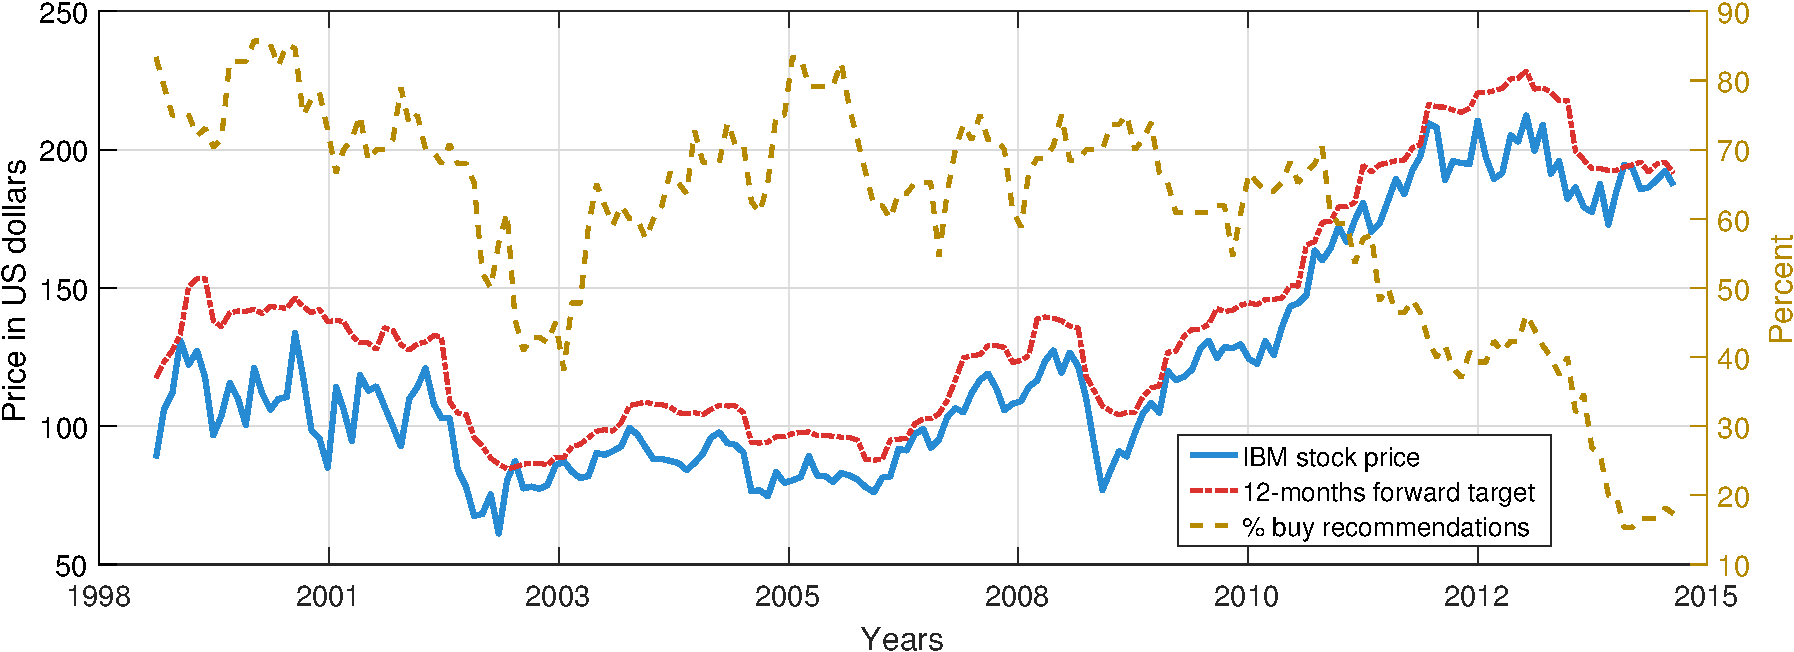
\includegraphics[width=1\linewidth]{../plots/IBM_price_plot}
	\caption[Spot price, 12 months forward target price and percentage of buy recommendations of the IBM stock (monthly data) between 1999 and 2015]{The figure shows IBM spot price, the mean 12 months forward target price and the percentage of buy recommendations from all recommendations (buy, sell, hold) of the IBM stock between 1999 and 2015.}
	\label{fig:ibmpriceplot}
\end{figure}

\begin{figure}[ht!]
	\centering
	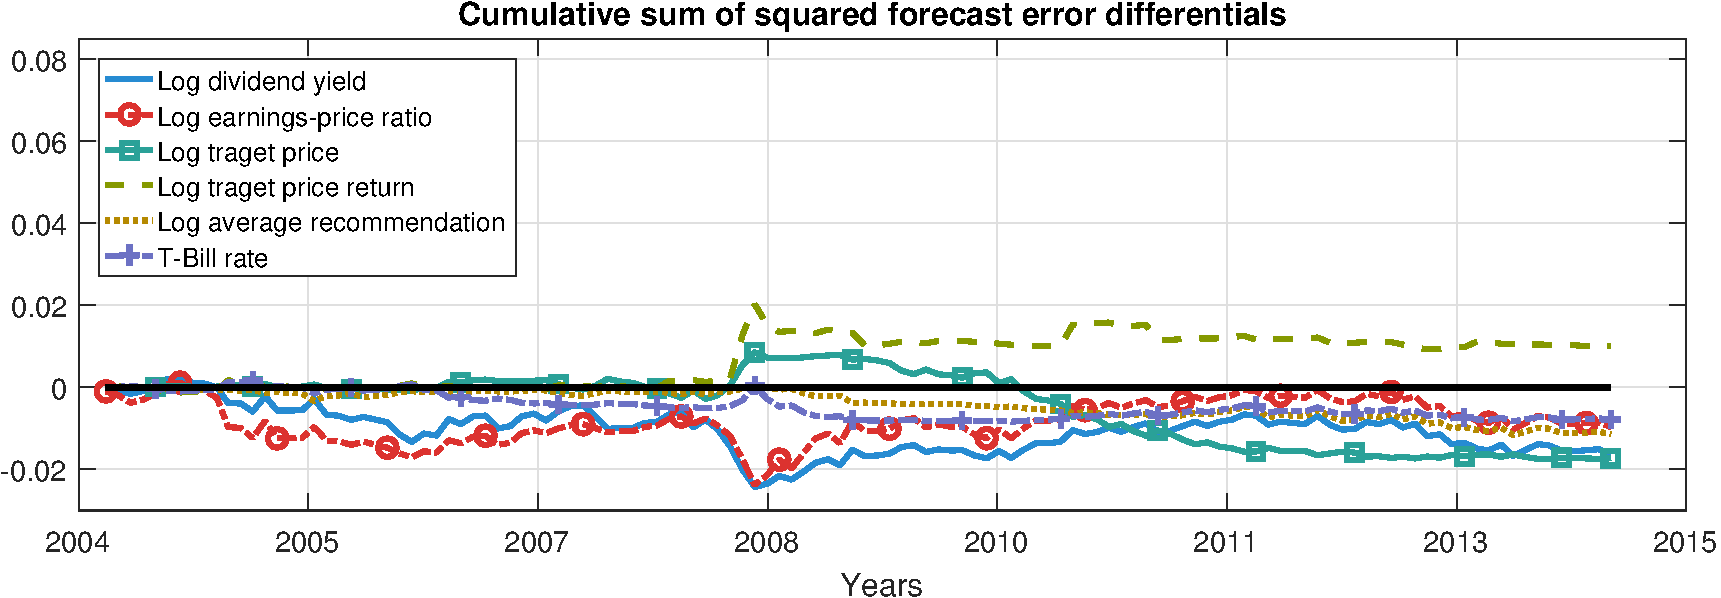
\includegraphics[width=1\linewidth]{../plots/IBM_CSSED_plot}
	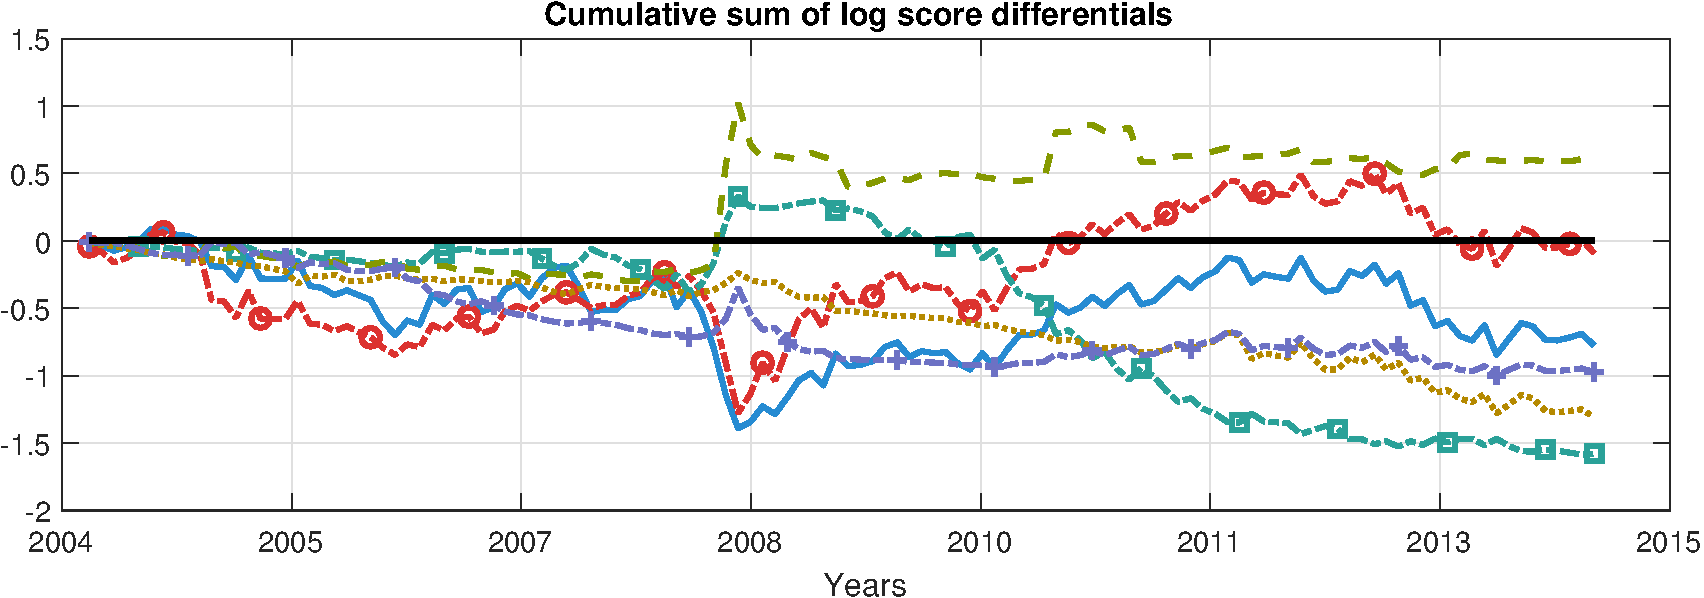
\includegraphics[width=1\linewidth]{../plots/IBM_CLSD_plot}
	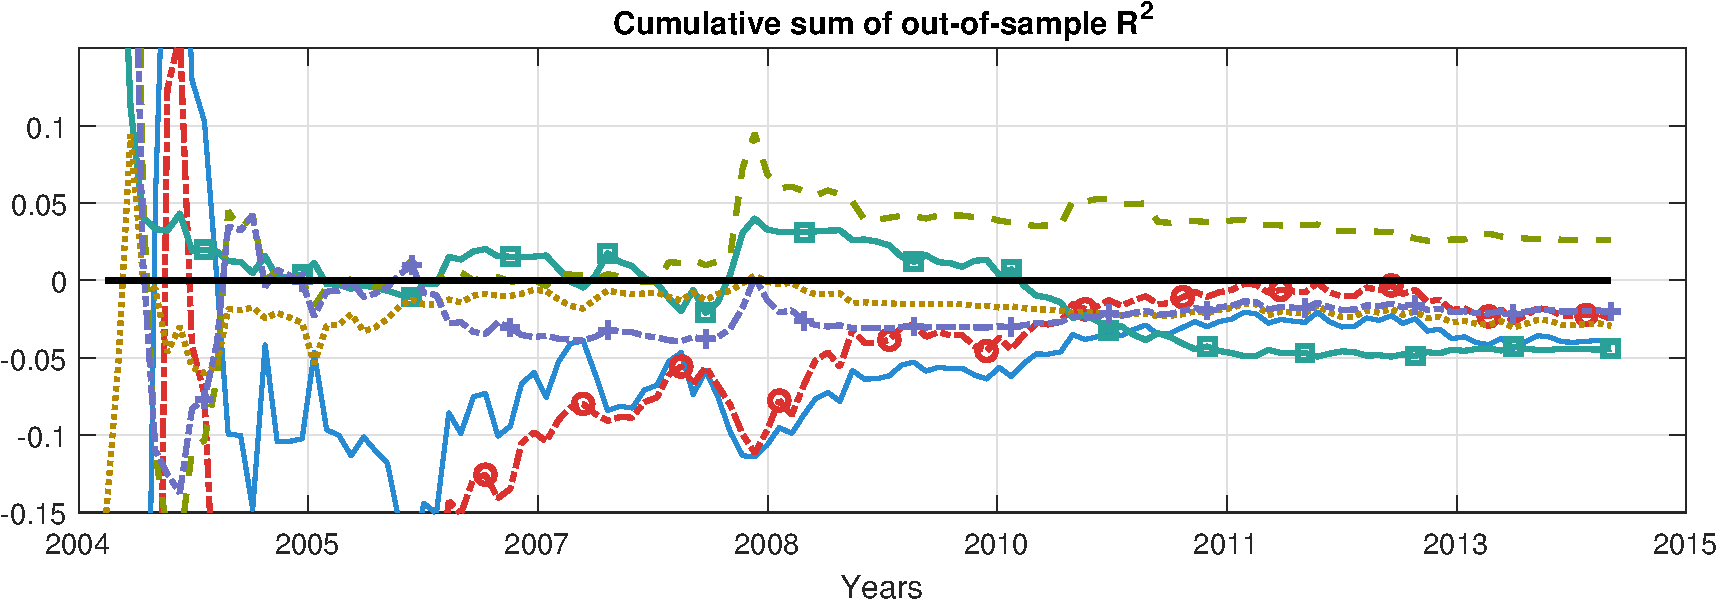
\includegraphics[width=1\linewidth]{../plots/IBM_R2_plot}
	\caption[Out-of-sample forecast performance results for different univariate models for the IBM stock for 2004 to 2015]{The figure provides out-of-sample forecast performance results for different univariate models for the IBM stock for 2004 to 2015. The top panel shows the cumulative sum of squared forecast errors of the benchmark mean model model minus the sum of squared forecast errors for six univariate models with different regressors, i.e. for model $m$ this is $\text{CSSED}_{m,t}=\sum_{i=S+1}^{t}\left(e_{0,i}^2-e_{m,i}^2\right)$. Each model is estimated from a linear regression of monthly excess returns on an intercept and a lagged predictor variable, i.e. $r_t=\alpha+\beta x_{t-1}+\varepsilon_t$. The middle panel shows the cumulative sum of log predictive scores of the six models minus the sum of log predictive scores of the benchmark mean model. The bottom panel shows the cumulative sum of out-of-sample $\text{R}^2$ values of each of the six univariate models. For all three panels it holds that values above zero indicate that a given predictor has better forecast performance than the benchmark model, while negative values suggest the opposite.}
	\label{fig:ibmclsdplot}
\end{figure}



\begin{figure}
	\centering
	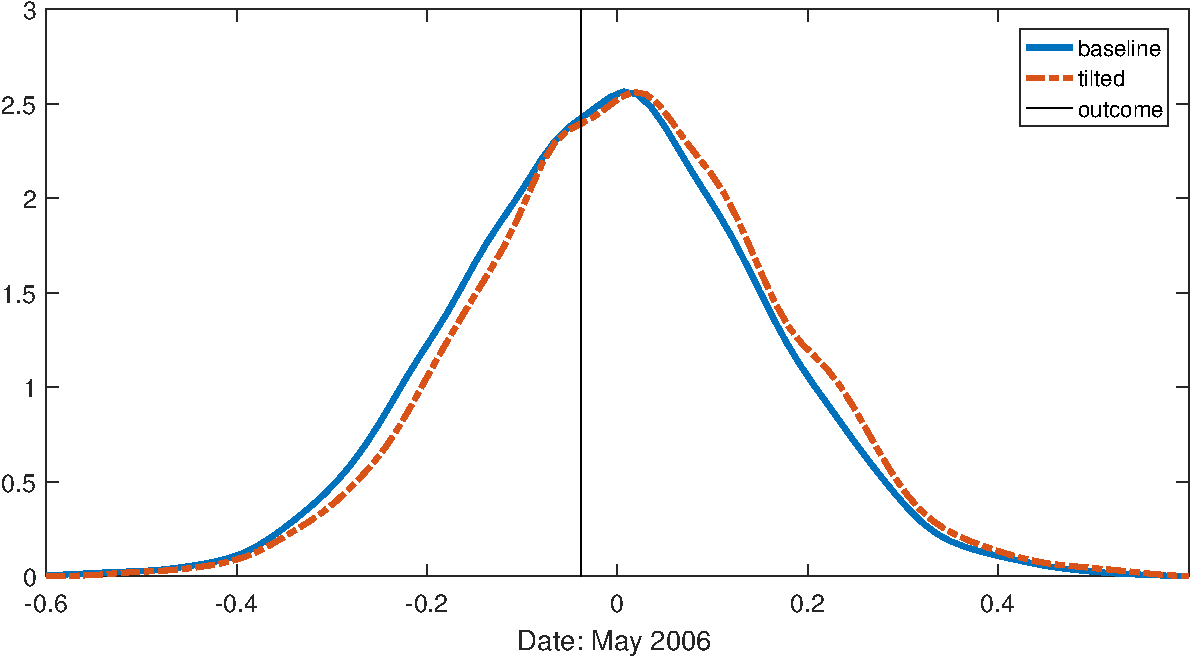
\includegraphics[width=0.49\linewidth]{../plots/IBM_density_m1}
	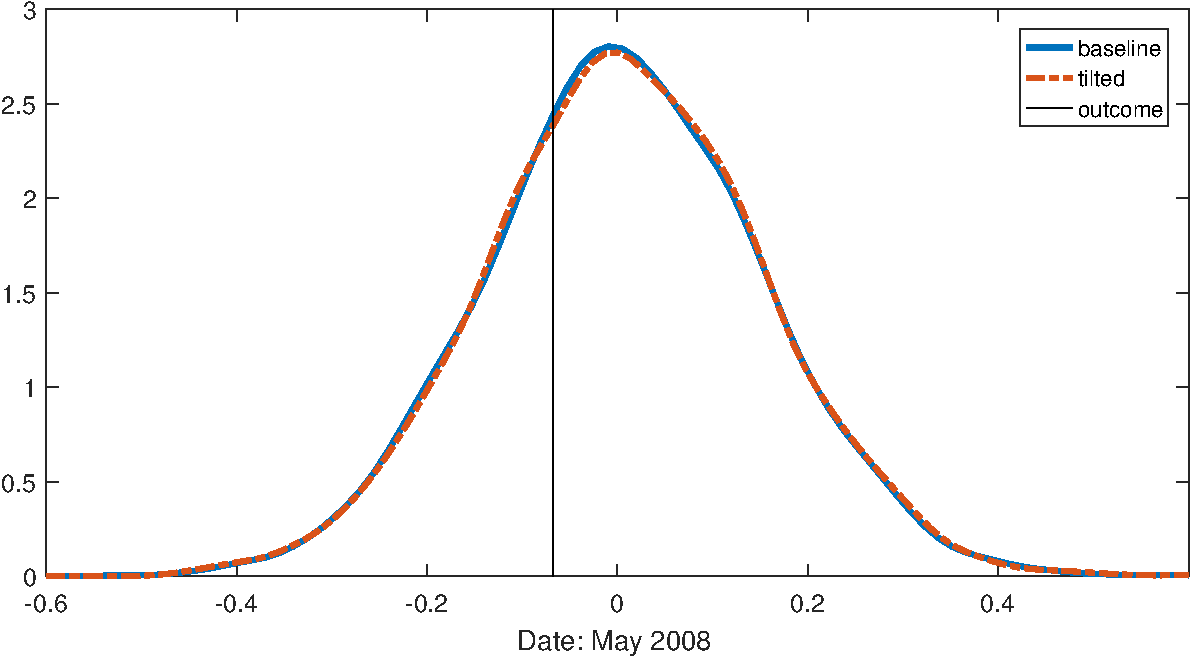
\includegraphics[width=0.49\linewidth]{../plots/IBM_density_m2}\\
	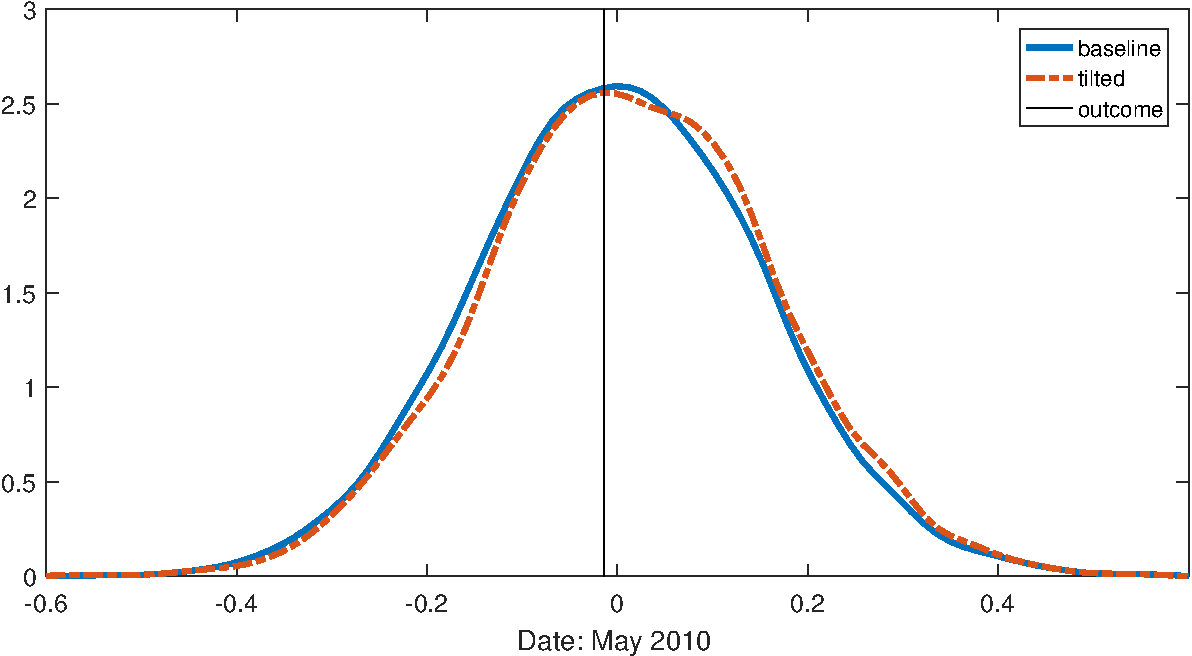
\includegraphics[width=0.49\linewidth]{../plots/IBM_density_m3}
	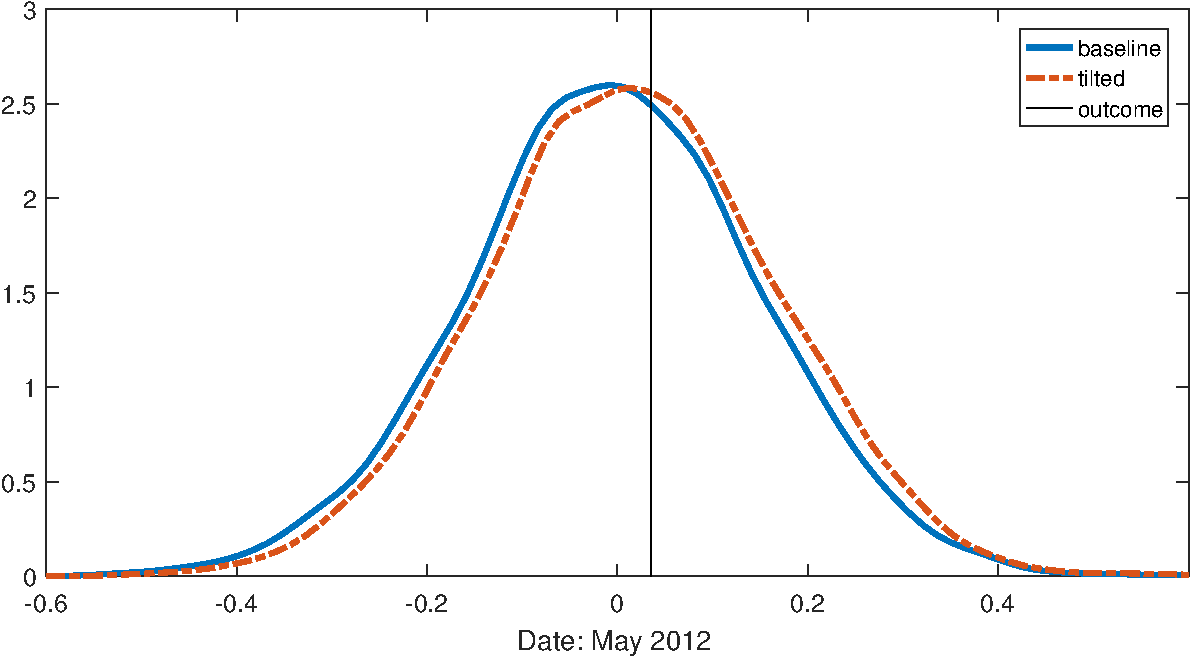
\includegraphics[width=0.49\linewidth]{../plots/IBM_density_m4}
	\caption[Kernel estimates of predictive density of the IBM returns from the TVPVAR(1) with dynamic model averaging and tilting towards the mean of monthly target price implied expected returns]{The figure shows the kernel of the predictive density of the IBM returns from the TVPVAR(1) model with dynamic model averaging and mean tilting towards the target price implied expected return at different times. The black horizontal line indicates the actual outcome return)}
	\label{fig:ibmdensitym}
\end{figure}

\begin{figure}
	\centering
	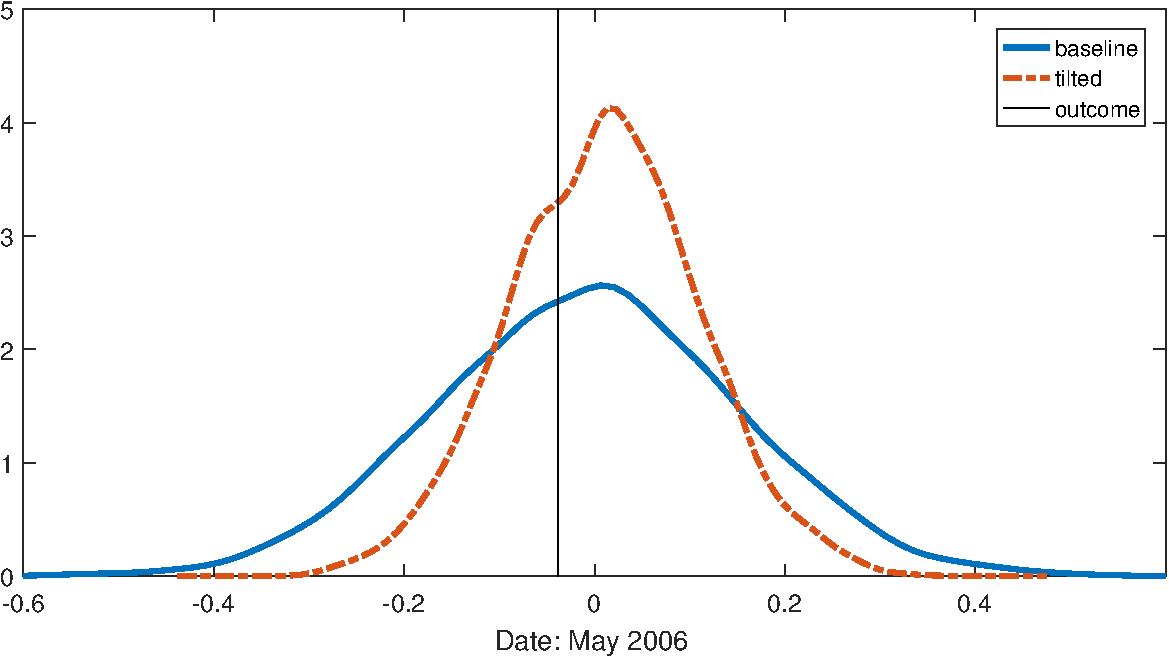
\includegraphics[width=0.49\linewidth]{../plots/IBM_density_mv1}
	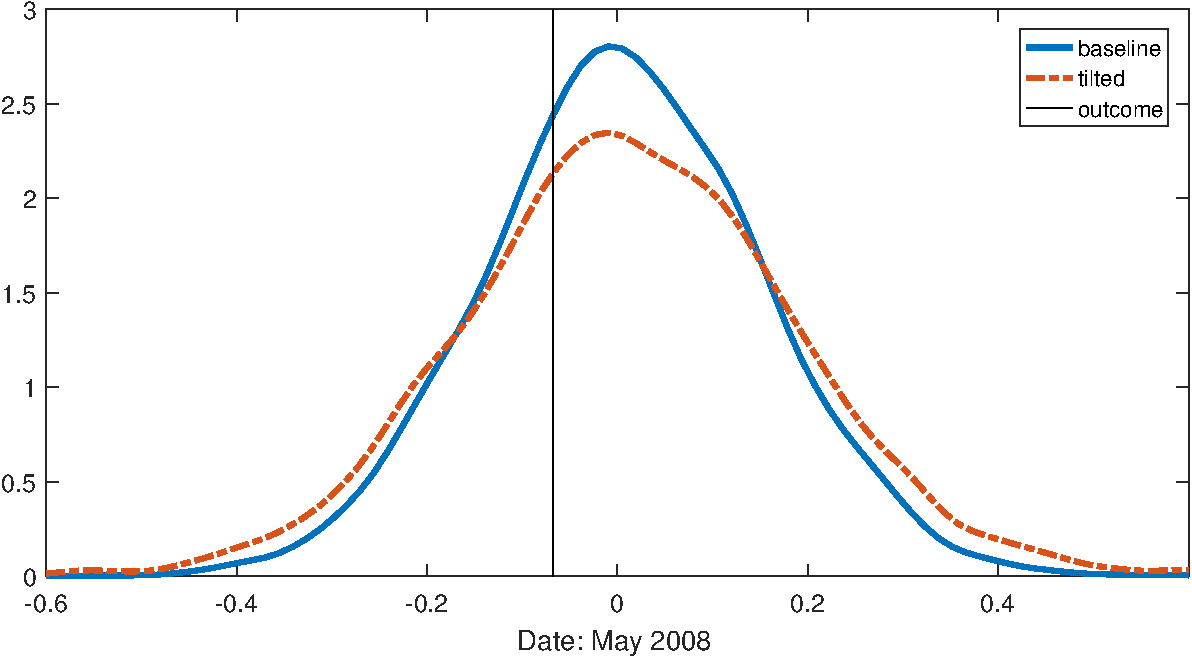
\includegraphics[width=0.49\linewidth]{../plots/IBM_density_mv2}\\
	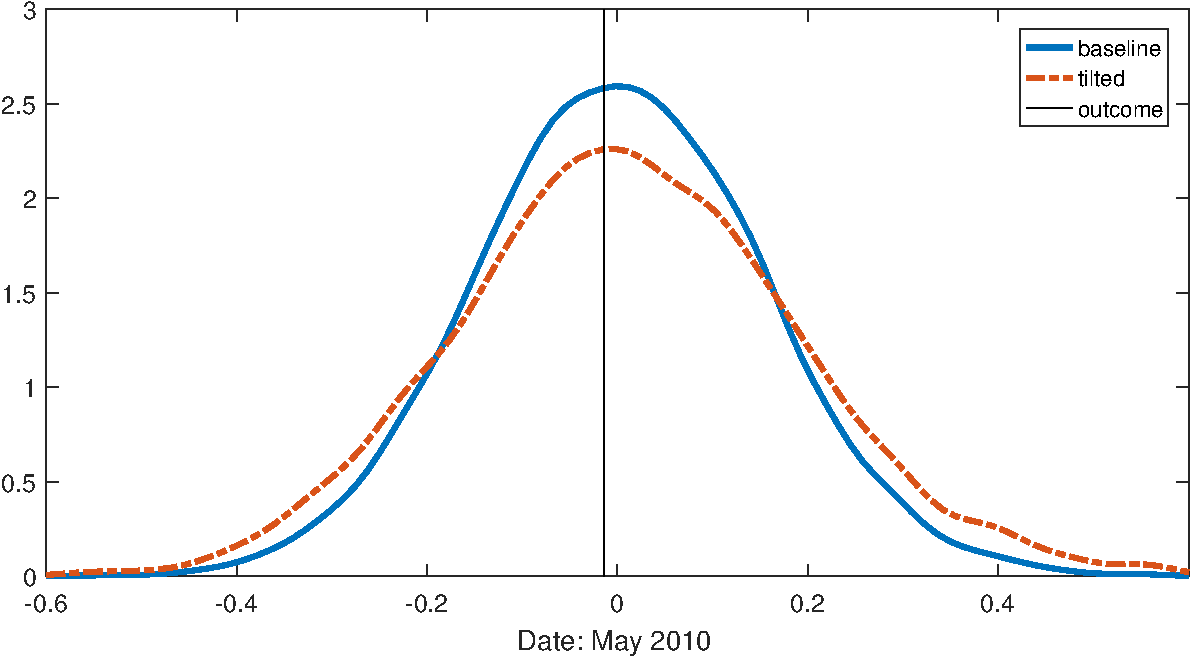
\includegraphics[width=0.49\linewidth]{../plots/IBM_density_mv3}
	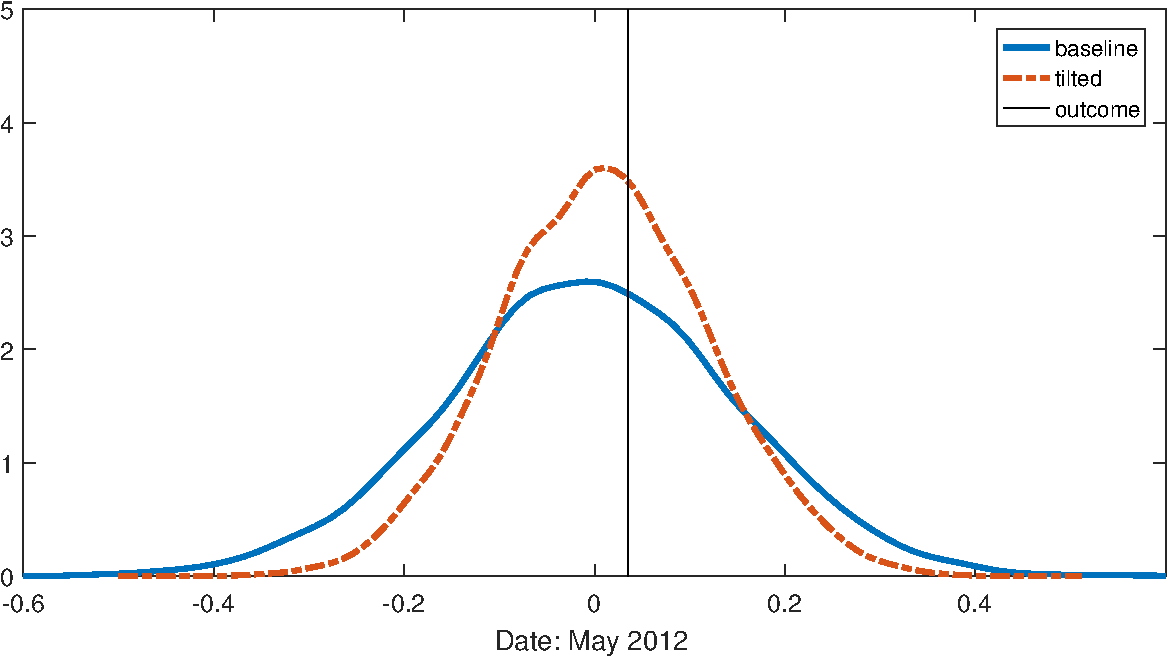
\includegraphics[width=0.49\linewidth]{../plots/IBM_density_mv4}
	\caption[Kernel estimates of predictive density of the IBM returns from the TVPVAR(1) with dynamic model averaging and tilting towards the mean and variance of monthly target price implied expected returns]{The figure shows the kernel of the predictive density of the IBM returns from the TVPVAR(1) model with dynamic model averaging with tilting towards the mean and variance of the target price implied expected returns at different times. The black horizontal line indicates the actual outcome return)}
	\label{fig:ibmdensitymv}
\end{figure}

\newpage\clearpage

\subsection{Tables}
\begin{table}[h!]
\fontsize{11}{18}\selectfont{
\begin{center}
\caption{Relative root mean squared errors between forecasted and observed spot prices for 20 Dow Jones constituents (sample: 1999 - 2015) }
\label{tab:rmsfe}
\vspace{-0.2cm}
\begin{tabularx}{1\textwidth}{@{}X@{\hspace{0.25cm}}c@{\hspace{0.25cm}}c@{\hspace{0.25cm}}c@{\hspace{0.25cm}}c@{\hspace{0.25cm}}c@{\hspace{0.25cm}}c@{\hspace{0.25cm}}c@{\hspace{0.25cm}}c@{\hspace{0.25cm}}c@{\hspace{0.25cm}}c@{}}
\toprule\toprule
 Stock  & AA	 & AAPL	 & AIG	 & AXP	 & BA	 & CAT	 & KO	 & DD	 & GE	 & HD	\\
\midrule
 rRMSFE  & $1.33^{**}$	 & \textbf{0.74}	 & $1.45^{***}$	 & \textbf{0.93}	 & \textbf{0.87}	 & \textbf{0.96}	 & 1.09	 & $1.24^{**}$	 & 1.23	 & \textbf{0.83}	\\
\midrule
\midrule
 Stock  & INTC	 & IBM	 & JNJ	 & MCD	 & MRK	 & MSFT	 & PG	 & UTX	 & WMT	 & DIS	\\
\midrule
 rRMSFE  & 1.36	 & \textbf{0.94}	 & \textbf{0.85}	 & $\mathbf{0.69^{***}}$	 & $1.25^{*}$	 & $1.65^{***}$	 & 1.01	 & \textbf{0.82}	 & 1.24	 & \textbf{0.84}	\\
\bottomrule\bottomrule
\end{tabularx}
\vspace{0.2cm}
\caption*{\footnotesize \textit{Note:} The table displays relative root mean squared errors between observed spot price twelve months ahead and the mean 12-month forward target price as well as the two year historical average for 20 Dow Jones constituents between 1999 and 2015. Values lower than one indicate that the target price generates superior forecast performance. For each stock, we test whether the target price forecast has lower MSFE than the average price forecast by the test proposed by \citet{giacomini2006}. One/two/three asterisks denote rejection of the null hypothesis of equal predictive ability at the ten/five/one percent test level.}
\end{center}}
\end{table}
\begin{table}[h!]
\fontsize{11}{18}\selectfont{
\begin{center}
\caption{Descriptive statistics on the returns, target prices and recommendations for 20 Dow Jones constituents (sample: 1999 - 2015) }
\label{tab:summary}
\vspace{-0.2cm}
\begin{tabularx}{1\textwidth}{@{}X@{\hspace{0.25cm}}c@{\hspace{0.25cm}}c@{\hspace{0.25cm}}c@{\hspace{0.25cm}}c@{\hspace{0.25cm}}c@{\hspace{0.25cm}}c@{\hspace{0.25cm}}c@{\hspace{0.25cm}}c@{\hspace{0.25cm}}c@{\hspace{0.25cm}}c@{}}
\toprule\toprule
 Stock  & AA	 & AAPL	 & AIG	 & AXP	 & BA	 & CAT	 & KO	 & DD	 & GE	 & HD	\\
\midrule
 Mean log ret  & -0.52	 & 2.01	 & -1.79	 & 0.26	 & 0.41	 & 0.43	 & -0.05	 & -0.18	 & -0.35	 & 0.27	\\
 Std log return  & 12.00	 & 14.13	 & 21.28	 & 9.52	 & 8.95	 & 10.13	 & 6.03	 & 8.27	 & 8.74	 & 8.22	\\
\midrule
 \# price tragets  & 14.38	 & 25.19	 & 13.17	 & 16.61	 & 16.18	 & 13.99	 & 13.11	 & 11.81	 & 13.33	 & 18.39	\\
 Mean exp ret  & 1.44	 & 1.44	 & 2.52	 & 1.12	 & 1.03	 & 1.08	 & 0.95	 & 1.30	 & 1.31	 & 1.10	\\
 Std exp ret  & 10.72	 & 7.49	 & 25.95	 & 6.08	 & 7.04	 & 7.20	 & 4.57	 & 5.79	 & 6.07	 & 6.37	\\
\midrule
 \# RECs  & 18.40	 & 32.33	 & 20.19	 & 21.36	 & 23.18	 & 20.09	 & 17.73	 & 16.48	 & 17.07	 & 25.76	\\
 Mean RECs  & 2.35	 & 2.13	 & 2.19	 & 2.36	 & 2.26	 & 2.29	 & 2.11	 & 2.40	 & 2.02	 & 2.11	\\
 Std RECs  & 0.38	 & 0.38	 & 0.58	 & 0.35	 & 0.38	 & 0.25	 & 0.25	 & 0.28	 & 0.34	 & 0.25	\\
\midrule
\midrule
 Stock  & INTC	 & IBM	 & JNJ	 & MCD	 & MRK	 & MSFT	 & PG	 & UTX	 & WMT	 & DIS	\\
\midrule
 Mean log ret  & -0.13	 & 0.14	 & 0.24	 & 0.27	 & -0.24	 & -0.09	 & 0.14	 & 0.39	 & 0.10	 & 0.40	\\
 Std log return  & 11.57	 & 7.76	 & 5.26	 & 6.54	 & 7.88	 & 8.90	 & 5.78	 & 7.25	 & 5.76	 & 7.91	\\
\midrule
 \# price tragets  & 28.66	 & 17.20	 & 14.66	 & 14.92	 & 15.53	 & 23.65	 & 13.34	 & 14.89	 & 17.98	 & 20.19	\\
 Mean exp ret  & 1.34	 & 0.95	 & 0.71	 & 1.10	 & 0.97	 & 1.53	 & 0.86	 & 0.95	 & 1.06	 & 1.26	\\
 Std exp ret  & 7.91	 & 5.29	 & 3.68	 & 5.40	 & 5.91	 & 6.91	 & 3.80	 & 4.52	 & 4.16	 & 6.62	\\
\midrule
 \# RECs  & 39.53	 & 23.10	 & 23.78	 & 20.60	 & 24.28	 & 32.73	 & 18.77	 & 19.98	 & 26.02	 & 27.22	\\
 Mean RECs  & 2.18	 & 2.18	 & 2.10	 & 2.16	 & 2.42	 & 1.91	 & 2.09	 & 1.95	 & 2.05	 & 2.29	\\
 Std RECs  & 0.29	 & 0.26	 & 0.25	 & 0.26	 & 0.36	 & 0.26	 & 0.21	 & 0.24	 & 0.25	 & 0.25	\\
\bottomrule\bottomrule
\end{tabularx}
\vspace{0.2cm}
\caption*{\footnotesize \textit{Note:} The table reports descriptive statistics on the returns, expected target returns and recommendations  for 20 Dow Jones constituents. It reports the mean and standard deviation of the logarithmic monthly returns, the mean number of available target prices, the mean and variance of the monthly forward target price implied expected return, i.e. simple returns between the spot and the twelve month forward target price at each point $t$ divided by 12, constructed from individual analyst data, the mean number of recommendations as well as the mean and standard deviation of the recommendations based on the 1 (strong buy) to 5 (strong sell) scale. Mean returns and standard deviations are multiplied by 100. Target prices and recommendations are obtained from I/B/E/S Datastream.}
\end{center}}
\end{table} 

%
%\begin{table}[h!]
\fontsize{11}{15}\selectfont{
\begin{center}
\caption{Forecast performance in terms of out-of-sample R$^2$ for 20 Dow Jones constituents (sample: 2004 - 2015) using a Bayesian VAR(1)}
\label{tab:mRsquard_BVAR}
\vspace{-0.2cm}
\begin{tabularx}{1\textwidth}{@{}X@{\hspace{0.2cm}}l@{\hspace{0.2cm}}l@{\hspace{0.2cm}}l@{\hspace{0.2cm}}l@{\hspace{0.2cm}}l@{\hspace{0.2cm}}l@{\hspace{0.2cm}}l@{\hspace{0.2cm}}l@{\hspace{0.2cm}}l@{\hspace{0.2cm}}l@{}}
\toprule\toprule
 Stock  & AA	 & AAPL	 & AIG	 & AXP	 & BA	 & CAT	 & KO	 & DD	 & GE	 & HD	\\
\midrule
 Log DY  & -6.90	 & \textbf{0.20}	 & -3.46	 & -0.68	 & -1.24	 & -0.51	 & -0.04	 & -0.20	 & -0.44	 & -0.13	\\
 Log EPR  & -1.97	 & \textbf{0.13}	 & -0.82	 & -0.30	 & -5.98	 & -0.06	 & -0.22	 & -0.16	 & -0.32	 & -0.62	\\
 Log DPR  & -0.13	 & -0.04	 & -0.05	 & -0.09	 & -1.09	 & \textbf{0.13}	 & -0.10	 & \textbf{0.25}	 & -0.13	 & -0.18	\\
 BMR  & -0.15	 & \textbf{0.21}	 & -1.18	 & -0.14	 & -0.13	 & -0.13	 & -0.73	 & -0.24	 & \textbf{0.00}	 & -0.06	\\
\midrule
 3M Tbill rate  & -0.10	 & \textbf{0.09}	 & -0.07	 & \textbf{0.33}	 & \textbf{0.06}	 & -0.18	 & -0.36	 & -0.28	 & -0.11	 & -0.17	\\
 Market return  & -0.09	 & \textbf{0.22}	 & -0.02	 & -0.06	 & -0.05	 & -0.12	 & -0.09	 & -0.21	 & -0.11	 & -0.57	\\
 LT yield  & -0.22	 & \textbf{0.03}	 & \textbf{0.24}	 & -0.15	 & -0.35	 & -0.27	 & -0.42	 & -0.28	 & -0.09	 & -0.29	\\
 CPI inflation  & -0.15	 & \textbf{0.18}	 & -0.10	 & -0.14	 & -0.13	 & -0.19	 & -0.30	 & -0.19	 & -0.20	 & \textbf{0.14}	\\
\midrule
 Log TPR  & -0.05	 & -0.16	 & -0.58	 & -0.45	 & -0.10	 & -0.13	 & -0.30	 & -0.17	 & -0.50	 & -0.20	\\
 Log TPV  & -0.24	 & \textbf{0.15}	 & -0.12	 & -0.17	 & -0.12	 & -0.53	 & -0.16	 & -0.19	 & -0.28	 & \textbf{0.28}	\\
 Log REC  & -0.54	 & \textbf{0.01}	 & -0.08	 & -0.48	 & -1.10	 & -0.31	 & -0.52	 & -0.72	 & -0.22	 & -0.08	\\
 Log REC return  & $\mathbf{8.06^{***}}$	 & -0.36	 & -0.09	 & \textbf{0.09}	 & -0.32	 & -0.01	 & $\mathbf{8.06^{***}}$	 & $\mathbf{8.06^{***}}$	 & -0.11	 & -0.02	\\
\midrule
\midrule
 Stock  & INTC	 & IBM	 & JNJ	 & MCD	 & MRK	 & MSFT	 & PG	 & UTX	 & WMT	 & DIS	\\
\midrule
 Log DY  & -0.35	 & -0.20	 & -0.46	 & -0.39	 & -0.31	 & -0.22	 & -0.43	 & -0.06	 & -0.23	 & -0.01	\\
 Log EPR  & -0.23	 & -0.19	 & -0.05	 & -0.51	 & -0.51	 & -0.11	 & \textbf{0.02}	 & -0.03	 & -0.44	 & -0.08	\\
 Log DPR  & -0.10	 & -0.45	 & -0.45	 & -0.50	 & -0.12	 & \textbf{0.09}	 & -1.70	 & \textbf{0.35}	 & -0.26	 & -0.03	\\
 BMR  & -0.12	 & -0.35	 & -0.15	 & -0.48	 & -0.12	 & -0.28	 & \textbf{0.03}	 & -0.06	 & -0.20	 & -0.06	\\
\midrule
 3M Tbill rate  & -0.36	 & -0.41	 & -0.64	 & -0.62	 & -0.32	 & -0.32	 & -0.13	 & -0.09	 & -0.17	 & \textbf{0.27}	\\
 Market return  & -0.39	 & -0.23	 & -0.07	 & -0.37	 & -0.16	 & -0.18	 & -0.52	 & -0.19	 & -0.23	 & -0.20	\\
 LT yield  & -0.39	 & -0.38	 & -0.25	 & -0.46	 & -0.40	 & -0.39	 & -0.73	 & -0.19	 & -0.32	 & -0.28	\\
 CPI inflation  & -0.14	 & -0.16	 & -0.06	 & -0.33	 & -0.22	 & -0.15	 & -0.40	 & -0.10	 & -0.14	 & -0.02	\\
\midrule
 Log TPR  & -0.02	 & -0.24	 & -0.03	 & \textbf{0.03}	 & -0.21	 & -0.00	 & -0.16	 & \textbf{0.05}	 & -0.26	 & \textbf{0.01}	\\
 Log TPV  & -0.18	 & -0.15	 & -0.07	 & -0.52	 & -0.18	 & -0.12	 & -0.48	 & -0.24	 & -0.24	 & \textbf{0.11}	\\
 Log REC  & -0.88	 & -0.38	 & -0.25	 & -1.07	 & -0.38	 & -0.38	 & -1.83	 & -1.16	 & -0.23	 & -0.34	\\
 Log REC return  & -0.59	 & -0.20	 & -0.05	 & -0.06	 & -0.03	 & -0.19	 & -0.14	 & -0.60	 & -0.15	 & -0.12	\\
\bottomrule\bottomrule
\end{tabularx}
\vspace{0.2cm}
\caption*{\footnotesize \textit{Note:} The table provides forecast performance results in terms of mean out-of-sample R$^2$ for 20 Dow Jones constituents (sample: 2004 - 2015) with a one month forecast horizon. The benchmark model is a simple mean model. For each asset, we estimate a Bayesian VAR system with constant coefficients using the Minnesota prior outlined in section 3 for the monthly excess returns on an intercept and a lagged predictor variable, i.e. $\begin{bmatrix}r_t\\x_t\end{bmatrix}=a+A_1\begin{bmatrix}r_{t-i}\\x_{t-i}\end{bmatrix}+\varepsilon_t$, $t=1,\ldots,T$. Further, DY is the dividend yield, PR is the earnings-price ratio, DPR is the dividend-price-ratio, BMR is the book-to-market ratio, LT is longterm yield, TPR is the target price return, TPV the target price variance and REC stands for recommendations. Values above zero indicate that a given predictor has better forecast performance than the benchmark model, while negative values suggest the opposite. All values are multiplied by 100. We test statistical significance in the average loss between the each model and a simple mean model using the \cite{diebold1995} test. One/two/three asterisks denote rejection of the null hypothesis of equal predictive ability at the ten/five/one percent test level.}
\end{center}}
\end{table} 
%\begin{table}[h!]
\fontsize{11}{15}\selectfont{
\begin{center}
\caption{Forecast performance in terms of cumulative sum of squared forecast errors for 20 Dow Jones constituents (sample: 2004 - 2015) using a Bayesian VAR(1)}
\label{tab:mCSSED_BVAR}
\vspace{-0.2cm}
\begin{tabularx}{1\textwidth}{@{}X@{\hspace{0.25cm}}l@{\hspace{0.25cm}}l@{\hspace{0.25cm}}l@{\hspace{0.25cm}}l@{\hspace{0.25cm}}l@{\hspace{0.25cm}}l@{\hspace{0.25cm}}l@{\hspace{0.25cm}}l@{\hspace{0.25cm}}l@{\hspace{0.25cm}}l@{}}
\toprule\toprule
 Stock  & AA	 & AAPL	 & AIG	 & AXP	 & BA	 & CAT	 & KO	 & DD	 & GE	 & HD	\\
\midrule
 Log DY  & -7.03	 & -0.09	 & -16.04	 & -0.20	 & -1.33	 & -0.15	 & -0.01	 & -0.03	 & -0.18	 & -0.03	\\
 Log EPR  & -0.97	 & -0.12	 & -0.33	 & -0.16	 & -20.63	 & -0.05	 & -0.01	 & -0.03	 & -0.09	 & -0.04	\\
 Log DPR  & -0.09	 & -0.07	 & -0.03	 & -0.15	 & -0.11	 & \textbf{0.00}	 & -0.01	 & \textbf{0.01}	 & -0.18	 & -0.03	\\
 BMR  & -0.17	 & \textbf{0.02}	 & -1.52	 & -0.05	 & -0.06	 & -0.07	 & -0.01	 & -0.04	 & -0.01	 & -0.01	\\
\midrule
 3M Tbill rate  & -0.06	 & -0.01	 & -0.31	 & -0.00	 & -0.04	 & -0.07	 & -0.02	 & -0.05	 & -0.05	 & -0.02	\\
 Market ret  & -0.04	 & \textbf{0.01}	 & -0.31	 & -0.04	 & -0.04	 & -0.05	 & -0.01	 & -0.03	 & -0.04	 & -0.01	\\
 LT yield  & -0.06	 & -0.04	 & \textbf{0.12}	 & -0.03	 & -0.03	 & -0.03	 & -0.01	 & -0.02	 & -0.02	 & -0.03	\\
 CPI inflation  & -0.10	 & -0.02	 & -0.45	 & -0.08	 & -0.05	 & -0.07	 & -0.01	 & -0.05	 & -0.08	 & -0.00	\\
\midrule
 Log TPR  & -0.04	 & -0.08	 & -1.82	 & -0.12	 & -0.03	 & -0.09	 & -0.01	 & -0.04	 & -0.11	 & -0.00	\\
 Log TPV  & -0.12	 & -0.03	 & -0.17	 & -0.08	 & -0.04	 & -0.15	 & -0.01	 & -0.05	 & -0.06	 & \textbf{0.01}	\\
 Log REC  & -0.11	 & -0.06	 & -0.21	 & -0.06	 & -0.10	 & -0.07	 & -0.01	 & -0.07	 & -0.04	 & -0.02	\\
 Log REC ret  & -0.09	 & -0.13	 & -0.40	 & \textbf{0.00}	 & -0.03	 & -0.05	 & -0.01	 & -0.04	 & -0.07	 & -0.01	\\
\midrule
\midrule
 Stock  & INTC	 & IBM	 & JNJ	 & MCD	 & MRK	 & MSFT	 & PG	 & UTX	 & WMT	 & DIS	\\
\midrule
 Log DY  & -0.03	 & -0.01	 & -0.02	 & -0.01	 & -0.03	 & -0.03	 & -0.02	 & -0.06	 & -0.01	 & -0.02	\\
 Log EPR  & -0.03	 & -0.01	 & -0.00	 & -0.01	 & -0.06	 & -0.02	 & -0.01	 & -0.02	 & -0.01	 & \textbf{0.02}	\\
 Log DPR  & -0.01	 & -0.02	 & -0.02	 & -0.03	 & -0.02	 & -0.01	 & -0.03	 & \textbf{0.01}	 & -0.00	 & -0.04	\\
 BMR  & -0.02	 & -0.01	 & -0.01	 & -0.00	 & -0.01	 & -0.03	 & -0.01	 & -0.02	 & -0.01	 & -0.01	\\
\midrule
 3M Tbill rate  & -0.05	 & -0.02	 & -0.01	 & -0.01	 & -0.03	 & -0.02	 & -0.02	 & -0.03	 & -0.01	 & \textbf{0.01}	\\
 Market ret  & -0.02	 & -0.00	 & -0.00	 & -0.01	 & -0.02	 & -0.00	 & -0.01	 & -0.01	 & -0.00	 & -0.01	\\
 LT yield  & -0.03	 & -0.02	 & -0.01	 & -0.02	 & -0.05	 & -0.04	 & -0.01	 & -0.02	 & -0.01	 & -0.01	\\
 CPI inflation  & -0.05	 & -0.02	 & -0.01	 & -0.01	 & -0.03	 & -0.02	 & -0.01	 & -0.03	 & -0.01	 & -0.03	\\
\midrule
 Log TPR  & -0.03	 & -0.01	 & -0.01	 & -0.00	 & -0.04	 & -0.03	 & -0.01	 & -0.01	 & -0.01	 & -0.04	\\
 Log TPV  & -0.08	 & -0.01	 & -0.01	 & -0.01	 & -0.04	 & -0.02	 & -0.02	 & -0.03	 & -0.02	 & -0.03	\\
 Log REC  & -0.07	 & -0.01	 & -0.01	 & -0.04	 & -0.03	 & -0.03	 & -0.01	 & -0.05	 & -0.01	 & -0.02	\\
 Log REC ret  & -0.03	 & -0.02	 & -0.01	 & -0.01	 & -0.04	 & -0.03	 & -0.01	 & -0.04	 & -0.01	 & -0.02	\\
\bottomrule\bottomrule
\end{tabularx}
\vspace{0.2cm}
\caption*{\footnotesize \textit{Note:} The table provides forecast performance results in terms of the mean cumulative sum of squared forecast errors between the benchmark mean model and a single regressor model for 20 Dow Jones constituents (sample: 2004 - 2015) with a one month forecast horizon. For each asset, we estimate a Bayesian VAR system with constant coefficients using the Minnesota prior outlined in section 3 for the monthly excess returns on an intercept and a lagged predictor variable, i.e. $\begin{bmatrix}r_t\\x_t\end{bmatrix}=a+A_1\begin{bmatrix}r_{t-i}\\x_{t-i}\end{bmatrix}+\varepsilon_t$, $t=1,\ldots,T$. Further, DY is the dividend yield, PR is the earnings-price ratio, DPR is the dividend-price-ratio, BMR is the book-to-market ratio, LT is longterm yield, TPR is the target price return, TPV the target price variance and REC stands for recommendations. Values above zero indicate that a given predictor has better forecast performance than the benchmark model, while negative values suggest the opposite. All values are multiplied by 100. We test statistical significance in the average loss between the each model and a simple mean model using the \cite{diebold1995} test. One/two/three asterisks denote rejection of the null hypothesis of equal predictive ability at the ten/five/one percent test level.}
\end{center}}
\end{table} 
%\begin{table}[h!]
\fontsize{11}{15}\selectfont{
\begin{center}
\caption{Forecast performance in terms of average log predictive score differentials for 20 Dow Jones constituents (sample: 2004 - 2015) using a Bayesian VAR(1)}
\label{tab:mCLSD_BVAR}
\vspace{-0.2cm}
\begin{tabularx}{1\textwidth}{@{}X@{\hspace{0.2cm}}l@{\hspace{0.2cm}}l@{\hspace{0.2cm}}l@{\hspace{0.2cm}}l@{\hspace{0.2cm}}l@{\hspace{0.2cm}}l@{\hspace{0.2cm}}l@{\hspace{0.2cm}}l@{\hspace{0.2cm}}l@{\hspace{0.2cm}}l@{}}
\toprule\toprule
 Stock  & AA	 & AAPL	 & AIG	 & AXP	 & BA	 & CAT	 & KO	 & DD	 & GE	 & HD	\\
\midrule
 Log DY  & -2.02	 & \textbf{0.04}	 & $\mathbf{7.14^{***}}$	 & -0.44	 & -0.23	 & -0.39	 & -0.00	 & -0.08	 & -0.25	 & -0.05	\\
 Log EPR  & -0.10	 & -0.01	 & $\mathbf{0.55^{*}}$	 & -0.16	 & -0.26	 & -0.06	 & -0.07	 & -0.05	 & -0.13	 & -0.15	\\
 Log DPR  & -0.09	 & -0.03	 & -0.28	 & -0.05	 & -0.33	 & \textbf{0.05}	 & \textbf{0.02}	 & \textbf{0.16}	 & -0.03	 & -0.06	\\
 BMR  & -0.03	 & \textbf{0.03}	 & $\mathbf{0.91^{*}}$	 & -0.07	 & -0.04	 & -0.06	 & -0.11	 & -0.07	 & \textbf{0.06}	 & -0.03	\\
\midrule
 3M Tbill rate  & \textbf{0.01}	 & -0.01	 & -0.46	 & \textbf{0.33}	 & \textbf{0.12}	 & -0.09	 & -0.06	 & -0.01	 & \textbf{0.05}	 & -0.05	\\
 Market return  & -0.06	 & \textbf{0.04}	 & -0.20	 & -0.03	 & -0.03	 & -0.09	 & \textbf{0.01}	 & -0.11	 & -0.03	 & -0.08	\\
 LT yield  & -0.09	 & \textbf{0.00}	 & -1.00	 & -0.03	 & -0.10	 & -0.18	 & -0.09	 & -0.08	 & \textbf{0.01}	 & -0.08	\\
 CPI inflation  & -0.12	 & \textbf{0.04}	 & -0.20	 & -0.10	 & -0.07	 & -0.17	 & -0.06	 & -0.09	 & -0.09	 & \textbf{0.02}	\\
\midrule
 Log TPR  & -0.02	 & -0.05	 & $\mathbf{0.67^{*}}$	 & -0.26	 & -0.05	 & -0.10	 & -0.08	 & -0.06	 & -0.26	 & -0.07	\\
 Log TPV  & -0.19	 & \textbf{0.01}	 & -0.20	 & -0.09	 & -0.06	 & -0.48	 & -0.04	 & -0.09	 & -0.14	 & \textbf{0.07}	\\
 Log REC  & -0.44	 & -0.04	 & -0.23	 & -0.27	 & -0.28	 & -0.26	 & -0.11	 & -0.29	 & -0.09	 & -0.03	\\
 Log REC return  & \textbf{0.00}	 & -0.16	 & -0.28	 & \textbf{0.08}	 & -0.12	 & -0.02	 & \textbf{0.00}	 & \textbf{0.00}	 & -0.03	 & \textbf{0.01}	\\
\midrule
\midrule
 Stock  & INTC	 & IBM	 & JNJ	 & MCD	 & MRK	 & MSFT	 & PG	 & UTX	 & WMT	 & DIS	\\
\midrule
 Log DY  & -0.08	 & -0.00	 & -0.08	 & -0.07	 & -0.11	 & -0.06	 & -0.05	 & -0.03	 & -0.05	 & -0.00	\\
 Log EPR  & -0.08	 & -0.04	 & -0.03	 & -0.01	 & -0.17	 & -0.03	 & -0.01	 & -0.03	 & -0.08	 & -0.05	\\
 Log DPR  & -0.01	 & -0.08	 & -0.06	 & -0.07	 & -0.03	 & \textbf{0.02}	 & -0.19	 & \textbf{0.13}	 & -0.04	 & \textbf{0.01}	\\
 BMR  & -0.06	 & -0.05	 & -0.01	 & -0.07	 & -0.04	 & -0.08	 & \textbf{0.01}	 & -0.03	 & -0.04	 & -0.02	\\
\midrule
 3M Tbill rate  & -0.09	 & -0.07	 & -0.08	 & -0.05	 & -0.09	 & -0.08	 & -0.04	 & -0.01	 & -0.01	 & \textbf{0.18}	\\
 Market return  & -0.08	 & -0.04	 & \textbf{0.03}	 & -0.05	 & -0.06	 & -0.06	 & \textbf{0.05}	 & -0.04	 & -0.04	 & -0.04	\\
 LT yield  & -0.09	 & -0.08	 & -0.06	 & -0.08	 & -0.11	 & -0.11	 & -0.11	 & -0.05	 & -0.07	 & -0.08	\\
 CPI inflation  & -0.06	 & -0.05	 & -0.03	 & -0.05	 & -0.09	 & -0.05	 & -0.06	 & -0.05	 & -0.04	 & -0.01	\\
\midrule
 Log TPR  & -0.03	 & -0.07	 & -0.02	 & -0.01	 & -0.08	 & -0.02	 & -0.04	 & -0.00	 & -0.06	 & \textbf{0.02}	\\
 Log TPV  & -0.07	 & -0.02	 & -0.02	 & -0.07	 & -0.06	 & -0.03	 & -0.07	 & -0.07	 & -0.05	 & \textbf{0.04}	\\
 Log REC  & -0.18	 & -0.07	 & -0.06	 & -0.14	 & -0.11	 & -0.10	 & -0.21	 & -0.23	 & -0.06	 & -0.10	\\
 Log REC return  & -0.02	 & -0.06	 & -0.03	 & -0.02	 & \textbf{0.00}	 & -0.07	 & -0.03	 & -0.14	 & -0.04	 & -0.04	\\
\bottomrule\bottomrule
\end{tabularx}
\vspace{0.2cm}
\caption*{\footnotesize \textit{Note:} The table provides forecast performance results in terms of average log predictive score differentials between the benchmark mean model and a single regressor model for 20 Dow Jones constituents (sample: 2004 - 2015) with a one month forecast horizon. For each asset, we estimate a Bayesian VAR system with constant coefficients using the Minnesota prior outlined in section 3 for the monthly excess returns on an intercept and a lagged predictor variable, i.e. $\begin{bmatrix}r_t\\x_t\end{bmatrix}=a+A_1\begin{bmatrix}r_{t-i}\\x_{t-i}\end{bmatrix}+\varepsilon_t$, $t=1,\ldots,T$. Further, DY is the dividend yield, PR is the earnings-price ratio, DPR is the dividend-price-ratio, BMR is the book-to-market ratio, LT is longterm yield, TPR is the target price return, TPV the target price variance and REC stands for recommendations. Values above zero indicate that a given predictor has better forecast performance than the benchmark model, while negative values suggest the opposite. All values are multiplied by 100. We test statistical significance in the average loss between the each model and a simple mean model using the \cite{diebold1995} test. One/two/three asterisks denote rejection of the null hypothesis of equal predictive ability at the ten/five/one percent test level.}
\end{center}}
\end{table} 
%\begin{table}[h!]
\fontsize{11}{15}\selectfont{
\begin{center}
\caption{Forecast performance in terms of the root mean squared forecast errors for 20 Dow Jones constituents (sample: 2004 - 2015) using a Bayesian VAR(1)}
\label{tab:mRMSFE_BVAR}
\vspace{-0.2cm}
\begin{tabularx}{1\textwidth}{@{}X@{\hspace{0.25cm}}l@{\hspace{0.25cm}}l@{\hspace{0.25cm}}l@{\hspace{0.25cm}}l@{\hspace{0.25cm}}l@{\hspace{0.25cm}}l@{\hspace{0.25cm}}l@{\hspace{0.25cm}}l@{\hspace{0.25cm}}l@{\hspace{0.25cm}}l@{}}
\toprule\toprule
 Stock  & AA	 & AAPL	 & AIG	 & AXP	 & BA	 & CAT	 & KO	 & DD	 & GE	 & HD	\\
\midrule
 Log DY  & \textbf{2.64}	 & \textbf{1.03}	 & \textbf{4.27}	 & \textbf{0.99}	 & \textbf{1.27}	 & \textbf{1.03}	 & \textbf{0.44}	 & \textbf{0.79}	 & \textbf{0.92}	 & \textbf{0.63}	\\
 Log EPR  & \textbf{1.44}	 & \textbf{1.05}	 & \textbf{2.36}	 & \textbf{0.98}	 & \textbf{4.14}	 & \textbf{0.99}	 & \textbf{0.44}	 & \textbf{0.79}	 & \textbf{0.88}	 & \textbf{0.64}	\\
 Log DPR  & \textbf{1.16}	 & \textbf{1.03}	 & \textbf{2.30}	 & \textbf{0.97}	 & \textbf{0.79}	 & \textbf{0.97}	 & \textbf{0.44}	 & \textbf{0.77}	 & \textbf{0.92}	 & \textbf{0.63}	\\
 BMR  & \textbf{1.19}	 & \textbf{0.99}	 & \textbf{2.55}	 & \textbf{0.93}	 & \textbf{0.76}	 & \textbf{1.00}	 & \textbf{0.45}	 & \textbf{0.79}	 & \textbf{0.84}	 & \textbf{0.62}	\\
\midrule
 3M Tbill rate  & \textbf{1.15}	 & \textbf{1.00}	 & \textbf{2.35}	 & \textbf{0.91}	 & \textbf{0.75}	 & \textbf{0.99}	 & \textbf{0.45}	 & \textbf{0.80}	 & \textbf{0.87}	 & \textbf{0.62}	\\
 Market ret  & \textbf{1.15}	 & \textbf{1.00}	 & \textbf{2.35}	 & \textbf{0.93}	 & \textbf{0.75}	 & \textbf{0.99}	 & \textbf{0.44}	 & \textbf{0.79}	 & \textbf{0.86}	 & \textbf{0.62}	\\
 LT yield  & \textbf{1.15}	 & \textbf{1.02}	 & \textbf{2.28}	 & \textbf{0.92}	 & \textbf{0.74}	 & \textbf{0.98}	 & \textbf{0.44}	 & \textbf{0.78}	 & \textbf{0.85}	 & \textbf{0.63}	\\
 CPI inflation  & \textbf{1.16}	 & \textbf{1.01}	 & \textbf{2.38}	 & \textbf{0.94}	 & \textbf{0.76}	 & \textbf{0.99}	 & \textbf{0.45}	 & \textbf{0.80}	 & \textbf{0.88}	 & \textbf{0.61}	\\
\midrule
 Log TPR  & \textbf{1.15}	 & \textbf{1.03}	 & \textbf{2.60}	 & \textbf{0.96}	 & \textbf{0.75}	 & \textbf{1.00}	 & \textbf{0.45}	 & \textbf{0.79}	 & \textbf{0.89}	 & \textbf{0.61}	\\
 Log TPV  & \textbf{1.17}	 & \textbf{1.01}	 & \textbf{2.33}	 & \textbf{0.94}	 & \textbf{0.75}	 & \textbf{1.03}	 & \textbf{0.45}	 & \textbf{0.80}	 & \textbf{0.87}	 & \textbf{0.61}	\\
 Log REC  & \textbf{1.17}	 & \textbf{1.02}	 & \textbf{2.33}	 & \textbf{0.93}	 & \textbf{0.78}	 & \textbf{1.00}	 & \textbf{0.45}	 & \textbf{0.81}	 & \textbf{0.86}	 & \textbf{0.62}	\\
 Log REC ret  & \textbf{1.16}	 & \textbf{1.05}	 & \textbf{2.37}	 & \textbf{0.91}	 & \textbf{0.74}	 & \textbf{0.99}	 & \textbf{0.44}	 & \textbf{0.79}	 & \textbf{0.87}	 & \textbf{0.62}	\\
\midrule
\midrule
 Stock  & INTC	 & IBM	 & JNJ	 & MCD	 & MRK	 & MSFT	 & PG	 & UTX	 & WMT	 & DIS	\\
\midrule
 Log DY  & \textbf{0.74}	 & \textbf{0.51}	 & \textbf{0.41}	 & \textbf{0.45}	 & \textbf{0.69}	 & \textbf{0.66}	 & \textbf{0.42}	 & \textbf{0.60}	 & \textbf{0.41}	 & \textbf{0.64}	\\
 Log EPR  & \textbf{0.74}	 & \textbf{0.51}	 & \textbf{0.40}	 & \textbf{0.45}	 & \textbf{0.71}	 & \textbf{0.66}	 & \textbf{0.41}	 & \textbf{0.58}	 & \textbf{0.41}	 & \textbf{0.62}	\\
 Log DPR  & \textbf{0.73}	 & \textbf{0.52}	 & \textbf{0.41}	 & \textbf{0.46}	 & \textbf{0.69}	 & \textbf{0.65}	 & \textbf{0.43}	 & \textbf{0.56}	 & \textbf{0.40}	 & \textbf{0.66}	\\
 BMR  & \textbf{0.74}	 & \textbf{0.51}	 & \textbf{0.40}	 & \textbf{0.44}	 & \textbf{0.68}	 & \textbf{0.66}	 & \textbf{0.41}	 & \textbf{0.58}	 & \textbf{0.41}	 & \textbf{0.64}	\\
\midrule
 3M Tbill rate  & \textbf{0.75}	 & \textbf{0.52}	 & \textbf{0.41}	 & \textbf{0.45}	 & \textbf{0.69}	 & \textbf{0.66}	 & \textbf{0.42}	 & \textbf{0.58}	 & \textbf{0.41}	 & \textbf{0.63}	\\
 Market ret  & \textbf{0.74}	 & \textbf{0.51}	 & \textbf{0.40}	 & \textbf{0.45}	 & \textbf{0.69}	 & \textbf{0.65}	 & \textbf{0.41}	 & \textbf{0.57}	 & \textbf{0.40}	 & \textbf{0.64}	\\
 LT yield  & \textbf{0.74}	 & \textbf{0.52}	 & \textbf{0.40}	 & \textbf{0.46}	 & \textbf{0.70}	 & \textbf{0.67}	 & \textbf{0.41}	 & \textbf{0.57}	 & \textbf{0.41}	 & \textbf{0.64}	\\
 CPI inflation  & \textbf{0.75}	 & \textbf{0.52}	 & \textbf{0.40}	 & \textbf{0.45}	 & \textbf{0.69}	 & \textbf{0.66}	 & \textbf{0.41}	 & \textbf{0.58}	 & \textbf{0.41}	 & \textbf{0.65}	\\
\midrule
 Log TPR  & \textbf{0.74}	 & \textbf{0.51}	 & \textbf{0.40}	 & \textbf{0.44}	 & \textbf{0.70}	 & \textbf{0.66}	 & \textbf{0.41}	 & \textbf{0.57}	 & \textbf{0.41}	 & \textbf{0.66}	\\
 Log TPV  & \textbf{0.77}	 & \textbf{0.51}	 & \textbf{0.40}	 & \textbf{0.45}	 & \textbf{0.69}	 & \textbf{0.66}	 & \textbf{0.42}	 & \textbf{0.58}	 & \textbf{0.42}	 & \textbf{0.65}	\\
 Log REC  & \textbf{0.76}	 & \textbf{0.51}	 & \textbf{0.40}	 & \textbf{0.47}	 & \textbf{0.69}	 & \textbf{0.66}	 & \textbf{0.42}	 & \textbf{0.59}	 & \textbf{0.41}	 & \textbf{0.64}	\\
 Log REC ret  & \textbf{0.74}	 & \textbf{0.52}	 & \textbf{0.40}	 & \textbf{0.44}	 & \textbf{0.70}	 & \textbf{0.66}	 & \textbf{0.41}	 & \textbf{0.59}	 & \textbf{0.41}	 & \textbf{0.64}	\\
\bottomrule\bottomrule
\end{tabularx}
\vspace{0.2cm}
\caption*{\footnotesize \textit{Note:} The table provides forecast performance results in terms of the root mean squared forecast errors between the benchmark mean model and a single regressor model for 20 Dow Jones constituents (sample: 2004 - 2015) with a one month forecast horizon. For each asset, we estimate a Bayesian VAR system with constant coefficients using the Minnesota prior outlined in section 3 for the monthly excess returns on an intercept and a lagged predictor variable, i.e. $\begin{bmatrix}r_t\\x_t\end{bmatrix}=a+A_1\begin{bmatrix}r_{t-i}\\x_{t-i}\end{bmatrix}+\varepsilon_t$, $t=1,\ldots,T$. Further, DY is the dividend yield, PR is the earnings-price ratio, DPR is the dividend-price-ratio, BMR is the book-to-market ratio, LT is longterm yield, TPR is the target price return, TPV the target price variance and REC stands for recommendations. Values above zero indicate that a given predictor has better forecast performance than the benchmark model, while negative values suggest the opposite. All values are multiplied by 100. We test statistical significance in the average loss between the each model and a simple mean model using the \cite{diebold1995} test. One/two/three asterisks denote rejection of the null hypothesis of equal predictive ability at the ten/five/one percent test level.}
\end{center}}
\end{table} 
%\begin{table}[h!]
\fontsize{11}{15}\selectfont{
\begin{center}
\caption{Forecast performance in terms of average continuously ranked probability score differentials for 20 Dow Jones constituents (sample: 2004 - 2015) using a Bayesian VAR(1)}
\label{tab:mCRPSD_BVAR}
\vspace{-0.2cm}
\begin{tabularx}{1\textwidth}{@{}X@{\hspace{0.25cm}}l@{\hspace{0.25cm}}l@{\hspace{0.25cm}}l@{\hspace{0.25cm}}l@{\hspace{0.25cm}}l@{\hspace{0.25cm}}l@{\hspace{0.25cm}}l@{\hspace{0.25cm}}l@{\hspace{0.25cm}}l@{\hspace{0.25cm}}l@{}}
\toprule\toprule
 Stock  & AA	 & AAPL	 & AIG	 & AXP	 & BA	 & CAT	 & KO	 & DD	 & GE	 & HD	\\
\midrule
 Log DY  & -3.58	 & -0.22	 & \textbf{23.65}	 & -1.50	 & -1.55	 & -0.83	 & -0.08	 & -0.12	 & -1.18	 & -0.18	\\
 Log EPR  & -0.23	 & -0.34	 & -2.04	 & -0.71	 & -2.52	 & -0.22	 & -0.09	 & -0.02	 & -0.30	 & -0.28	\\
 Log DPR  & -0.22	 & \textbf{0.05}	 & -0.41	 & -0.81	 & -0.45	 & -0.07	 & -0.03	 & \textbf{0.05}	 & -0.79	 & -0.24	\\
 BMR  & -0.38	 & \textbf{0.10}	 & \textbf{2.40}	 & -0.20	 & -0.24	 & -0.29	 & -0.12	 & -0.07	 & -0.23	 & -0.07	\\
\midrule
 3M Tbill rate  & \textbf{0.07}	 & \textbf{0.06}	 & -0.70	 & \textbf{0.44}	 & \textbf{0.04}	 & -0.24	 & -0.11	 & \textbf{0.10}	 & \textbf{0.02}	 & -0.08	\\
 Market ret  & -0.06	 & \textbf{0.08}	 & -0.40	 & -0.14	 & -0.25	 & -0.26	 & -0.02	 & -0.06	 & -0.09	 & \textbf{0.00}	\\
 LT yield  & -0.01	 & \textbf{0.08}	 & -1.99	 & -0.07	 & -0.22	 & -0.15	 & -0.03	 & \textbf{0.01}	 & \textbf{0.11}	 & -0.17	\\
 CPI inflation  & -0.36	 & -0.03	 & \textbf{0.17}	 & -0.53	 & -0.38	 & -0.36	 & -0.17	 & -0.22	 & -0.44	 & -0.05	\\
\midrule
 Log TPR  & -0.02	 & -0.09	 & \textbf{6.90}	 & -0.76	 & -0.19	 & -0.43	 & -0.14	 & -0.18	 & -0.51	 & -0.02	\\
 Log TPV  & -0.36	 & -0.11	 & -0.77	 & -0.26	 & -0.26	 & -0.79	 & -0.14	 & -0.19	 & -0.35	 & \textbf{0.08}	\\
 Log REC  & -0.40	 & -0.03	 & -0.05	 & -0.28	 & -0.44	 & -0.49	 & -0.13	 & -0.29	 & -0.17	 & -0.16	\\
 Log REC ret  & -0.27	 & -0.24	 & -0.08	 & -0.02	 & -0.18	 & -0.08	 & -0.06	 & -0.15	 & -0.26	 & -0.05	\\
\midrule
\midrule
 Stock  & INTC	 & IBM	 & JNJ	 & MCD	 & MRK	 & MSFT	 & PG	 & UTX	 & WMT	 & DIS	\\
\midrule
 Log DY  & -0.11	 & \textbf{0.00}	 & -0.18	 & -0.08	 & -0.14	 & -0.17	 & -0.20	 & -0.59	 & -0.04	 & -0.15	\\
 Log EPR  & -0.14	 & -0.11	 & -0.05	 & -0.10	 & -0.28	 & -0.08	 & -0.08	 & -0.21	 & -0.14	 & \textbf{0.08}	\\
 Log DPR  & \textbf{0.04}	 & -0.16	 & -0.17	 & -0.16	 & -0.09	 & -0.02	 & -0.36	 & \textbf{0.06}	 & \textbf{0.00}	 & -0.28	\\
 BMR  & -0.07	 & -0.04	 & -0.04	 & \textbf{0.02}	 & -0.05	 & -0.20	 & -0.07	 & -0.18	 & -0.11	 & -0.08	\\
\midrule
 3M Tbill rate  & -0.16	 & -0.03	 & -0.05	 & -0.08	 & -0.08	 & -0.02	 & -0.16	 & -0.09	 & -0.07	 & \textbf{0.17}	\\
 Market ret  & -0.07	 & -0.05	 & -0.02	 & -0.07	 & -0.10	 & \textbf{0.01}	 & -0.05	 & -0.13	 & -0.03	 & -0.10	\\
 LT yield  & -0.07	 & -0.13	 & -0.09	 & -0.13	 & -0.18	 & -0.17	 & -0.10	 & -0.14	 & -0.12	 & -0.07	\\
 CPI inflation  & -0.13	 & -0.18	 & -0.12	 & -0.12	 & -0.12	 & -0.10	 & -0.12	 & -0.27	 & -0.09	 & -0.26	\\
\midrule
 Log TPR  & -0.09	 & -0.12	 & -0.11	 & -0.06	 & -0.22	 & -0.19	 & -0.09	 & -0.10	 & -0.13	 & -0.20	\\
 Log TPV  & -0.22	 & -0.07	 & -0.11	 & -0.12	 & -0.16	 & -0.08	 & -0.16	 & -0.30	 & -0.23	 & -0.16	\\
 Log REC  & -0.23	 & -0.02	 & -0.07	 & -0.17	 & -0.14	 & -0.11	 & -0.11	 & -0.30	 & -0.11	 & -0.17	\\
 Log REC ret  & -0.07	 & -0.15	 & -0.08	 & -0.08	 & -0.16	 & -0.26	 & -0.10	 & -0.32	 & -0.09	 & -0.15	\\
\bottomrule\bottomrule
\end{tabularx}
\vspace{0.2cm}
\caption*{\footnotesize \textit{Note:} The table provides forecast performance results in terms of average continuously ranked probability score differentials between the benchmark mean model and a single regressor model for 20 Dow Jones constituents (sample: 2004 - 2015) with a one month forecast horizon. For each asset, we estimate a Bayesian VAR system with constant coefficients using the Minnesota prior outlined in section 3 for the monthly excess returns on an intercept and a lagged predictor variable, i.e. $\begin{bmatrix}r_t\\x_t\end{bmatrix}=a+A_1\begin{bmatrix}r_{t-i}\\x_{t-i}\end{bmatrix}+\varepsilon_t$, $t=1,\ldots,T$. Further, DY is the dividend yield, PR is the earnings-price ratio, DPR is the dividend-price-ratio, BMR is the book-to-market ratio, LT is longterm yield, TPR is the target price return, TPV the target price variance and REC stands for recommendations. Values above zero indicate that a given predictor has better forecast performance than the benchmark model, while negative values suggest the opposite. All values are multiplied by 100. We test statistical significance in the average loss between the each model and a simple mean model using the \cite{diebold1995} test. One/two/three asterisks denote rejection of the null hypothesis of equal predictive ability at the ten/five/one percent test level.}
\end{center}}
\end{table} 

\newpage
\begin{table}[h!]
\fontsize{11}{15}\selectfont{
\begin{center}
\caption{Forecast performance in terms of out-of-sample R$^2$ for 20 Dow Jones constituents (sample: 2004 - 2015) using a Bayesian VAR(1)}
\label{tab:mRsquard_BVAR}
\vspace{-0.2cm}
\begin{tabularx}{1\textwidth}{@{}X@{\hspace{0.2cm}}l@{\hspace{0.2cm}}l@{\hspace{0.2cm}}l@{\hspace{0.2cm}}l@{\hspace{0.2cm}}l@{\hspace{0.2cm}}l@{\hspace{0.2cm}}l@{\hspace{0.2cm}}l@{\hspace{0.2cm}}l@{\hspace{0.2cm}}l@{}}
\toprule\toprule
 Stock  & AA	 & AAPL	 & AIG	 & AXP	 & BA	 & CAT	 & KO	 & DD	 & GE	 & HD	\\
\midrule
 Log DY  & -6.90	 & \textbf{0.20}	 & -3.46	 & -0.68	 & -1.24	 & -0.51	 & -0.04	 & -0.20	 & -0.44	 & -0.13	\\
 Log EPR  & -1.97	 & \textbf{0.13}	 & -0.82	 & -0.30	 & -5.98	 & -0.06	 & -0.22	 & -0.16	 & -0.32	 & -0.62	\\
 Log DPR  & -0.13	 & -0.04	 & -0.05	 & -0.09	 & -1.09	 & \textbf{0.13}	 & -0.10	 & \textbf{0.25}	 & -0.13	 & -0.18	\\
 BMR  & -0.15	 & \textbf{0.21}	 & -1.18	 & -0.14	 & -0.13	 & -0.13	 & -0.73	 & -0.24	 & \textbf{0.00}	 & -0.06	\\
\midrule
 3M Tbill rate  & -0.10	 & \textbf{0.09}	 & -0.07	 & \textbf{0.33}	 & \textbf{0.06}	 & -0.18	 & -0.36	 & -0.28	 & -0.11	 & -0.17	\\
 Market return  & -0.09	 & \textbf{0.22}	 & -0.02	 & -0.06	 & -0.05	 & -0.12	 & -0.09	 & -0.21	 & -0.11	 & -0.57	\\
 LT yield  & -0.22	 & \textbf{0.03}	 & \textbf{0.24}	 & -0.15	 & -0.35	 & -0.27	 & -0.42	 & -0.28	 & -0.09	 & -0.29	\\
 CPI inflation  & -0.15	 & \textbf{0.18}	 & -0.10	 & -0.14	 & -0.13	 & -0.19	 & -0.30	 & -0.19	 & -0.20	 & \textbf{0.14}	\\
\midrule
 Log TPR  & -0.05	 & -0.16	 & -0.58	 & -0.45	 & -0.10	 & -0.13	 & -0.30	 & -0.17	 & -0.50	 & -0.20	\\
 Log TPV  & -0.24	 & \textbf{0.15}	 & -0.12	 & -0.17	 & -0.12	 & -0.53	 & -0.16	 & -0.19	 & -0.28	 & \textbf{0.28}	\\
 Log REC  & -0.54	 & \textbf{0.01}	 & -0.08	 & -0.48	 & -1.10	 & -0.31	 & -0.52	 & -0.72	 & -0.22	 & -0.08	\\
 Log REC return  & $\mathbf{8.06^{***}}$	 & -0.36	 & -0.09	 & \textbf{0.09}	 & -0.32	 & -0.01	 & $\mathbf{8.06^{***}}$	 & $\mathbf{8.06^{***}}$	 & -0.11	 & -0.02	\\
\midrule
\midrule
 Stock  & INTC	 & IBM	 & JNJ	 & MCD	 & MRK	 & MSFT	 & PG	 & UTX	 & WMT	 & DIS	\\
\midrule
 Log DY  & -0.35	 & -0.20	 & -0.46	 & -0.39	 & -0.31	 & -0.22	 & -0.43	 & -0.06	 & -0.23	 & -0.01	\\
 Log EPR  & -0.23	 & -0.19	 & -0.05	 & -0.51	 & -0.51	 & -0.11	 & \textbf{0.02}	 & -0.03	 & -0.44	 & -0.08	\\
 Log DPR  & -0.10	 & -0.45	 & -0.45	 & -0.50	 & -0.12	 & \textbf{0.09}	 & -1.70	 & \textbf{0.35}	 & -0.26	 & -0.03	\\
 BMR  & -0.12	 & -0.35	 & -0.15	 & -0.48	 & -0.12	 & -0.28	 & \textbf{0.03}	 & -0.06	 & -0.20	 & -0.06	\\
\midrule
 3M Tbill rate  & -0.36	 & -0.41	 & -0.64	 & -0.62	 & -0.32	 & -0.32	 & -0.13	 & -0.09	 & -0.17	 & \textbf{0.27}	\\
 Market return  & -0.39	 & -0.23	 & -0.07	 & -0.37	 & -0.16	 & -0.18	 & -0.52	 & -0.19	 & -0.23	 & -0.20	\\
 LT yield  & -0.39	 & -0.38	 & -0.25	 & -0.46	 & -0.40	 & -0.39	 & -0.73	 & -0.19	 & -0.32	 & -0.28	\\
 CPI inflation  & -0.14	 & -0.16	 & -0.06	 & -0.33	 & -0.22	 & -0.15	 & -0.40	 & -0.10	 & -0.14	 & -0.02	\\
\midrule
 Log TPR  & -0.02	 & -0.24	 & -0.03	 & \textbf{0.03}	 & -0.21	 & -0.00	 & -0.16	 & \textbf{0.05}	 & -0.26	 & \textbf{0.01}	\\
 Log TPV  & -0.18	 & -0.15	 & -0.07	 & -0.52	 & -0.18	 & -0.12	 & -0.48	 & -0.24	 & -0.24	 & \textbf{0.11}	\\
 Log REC  & -0.88	 & -0.38	 & -0.25	 & -1.07	 & -0.38	 & -0.38	 & -1.83	 & -1.16	 & -0.23	 & -0.34	\\
 Log REC return  & -0.59	 & -0.20	 & -0.05	 & -0.06	 & -0.03	 & -0.19	 & -0.14	 & -0.60	 & -0.15	 & -0.12	\\
\bottomrule\bottomrule
\end{tabularx}
\vspace{0.2cm}
\caption*{\footnotesize \textit{Note:} The table provides forecast performance results in terms of mean out-of-sample R$^2$ for 20 Dow Jones constituents (sample: 2004 - 2015) with a one month forecast horizon. The benchmark model is a simple mean model. For each asset, we estimate a Bayesian VAR system with constant coefficients using the Minnesota prior outlined in section 3 for the monthly excess returns on an intercept and a lagged predictor variable, i.e. $\begin{bmatrix}r_t\\x_t\end{bmatrix}=a+A_1\begin{bmatrix}r_{t-i}\\x_{t-i}\end{bmatrix}+\varepsilon_t$, $t=1,\ldots,T$. Further, DY is the dividend yield, PR is the earnings-price ratio, DPR is the dividend-price-ratio, BMR is the book-to-market ratio, LT is longterm yield, TPR is the target price return, TPV the target price variance and REC stands for recommendations. Values above zero indicate that a given predictor has better forecast performance than the benchmark model, while negative values suggest the opposite. All values are multiplied by 100. We test statistical significance in the average loss between the each model and a simple mean model using the \cite{diebold1995} test. One/two/three asterisks denote rejection of the null hypothesis of equal predictive ability at the ten/five/one percent test level.}
\end{center}}
\end{table} 
\begin{table}[h!]
\fontsize{11}{15}\selectfont{
\begin{center}
\caption{Forecast performance in terms of out-of-sample R$^2$ for 20 Dow Jones constituents (sample: 2004 - 2015) using a TVP-BVAR(1) with stochastic volatility}
\label{tab:mRsquard_TVPVAR}
\vspace{-0.2cm}
\begin{tabularx}{1\textwidth}{@{}X@{\hspace{0.2cm}}l@{\hspace{0.2cm}}l@{\hspace{0.2cm}}l@{\hspace{0.2cm}}l@{\hspace{0.2cm}}l@{\hspace{0.2cm}}l@{\hspace{0.2cm}}l@{\hspace{0.2cm}}l@{\hspace{0.2cm}}l@{\hspace{0.2cm}}l@{}}
\toprule\toprule
 Stock  & AA	 & AAPL	 & AIG	 & AXP	 & BA	 & CAT	 & KO	 & DD	 & GE	 & HD	\\
\midrule
 Log DY  & -6.49	 & \textbf{0.68}	 & -3.12	 & -0.33	 & -0.89	 & -0.14	 & \textbf{0.36}	 & \textbf{0.26}	 & -0.15	 & \textbf{0.21}	\\
 Log EPR  & -1.52	 & \textbf{0.37}	 & -0.44	 & -0.14	 & -5.60	 & \textbf{0.06}	 & -0.10	 & -0.01	 & -0.08	 & -0.25	\\
 Log DPR  & -0.07	 & \textbf{0.36}	 & \textbf{0.32}	 & \textbf{0.39}	 & -0.95	 & \textbf{0.39}	 & \textbf{0.36}	 & \textbf{0.63}	 & -0.12	 & \textbf{0.04}	\\
 BMR  & \textbf{0.30}	 & \textbf{0.28}	 & -0.99	 & -0.12	 & \textbf{0.21}	 & \textbf{0.22}	 & -0.56	 & \textbf{0.14}	 & \textbf{0.17}	 & -0.02	\\
\midrule
 3M Tbill rate  & \textbf{0.21}	 & \textbf{0.30}	 & \textbf{0.26}	 & \textbf{0.55}	 & \textbf{0.39}	 & \textbf{0.27}	 & -0.26	 & -0.09	 & -0.03	 & -0.06	\\
 Market return  & -0.04	 & \textbf{0.67}	 & \textbf{0.06}	 & \textbf{0.13}	 & \textbf{0.03}	 & \textbf{0.36}	 & \textbf{0.03}	 & \textbf{0.07}	 & \textbf{0.28}	 & -0.11	\\
 LT yield  & -0.08	 & \textbf{0.42}	 & \textbf{0.59}	 & \textbf{0.23}	 & -0.29	 & \textbf{0.00}	 & -0.11	 & -0.24	 & \textbf{0.06}	 & -0.22	\\
 CPI inflation  & \textbf{0.13}	 & \textbf{0.66}	 & -0.09	 & \textbf{0.25}	 & \textbf{0.12}	 & -0.12	 & -0.07	 & -0.16	 & \textbf{0.07}	 & \textbf{0.55}	\\
\midrule
 Log TPR  & \textbf{0.47}	 & \textbf{0.35}	 & -0.41	 & -0.26	 & \textbf{0.38}	 & \textbf{0.24}	 & \textbf{0.31}	 & \textbf{0.36}	 & \textbf{0.18}	 & \textbf{0.01}	\\
 Log TPV  & \textbf{0.30}	 & \textbf{0.90}	 & \textbf{0.44}	 & -0.08	 & \textbf{0.24}	 & -0.00	 & \textbf{0.12}	 & \textbf{0.15}	 & \textbf{0.39}	 & \textbf{0.77}	\\
 Log REC  & -0.46	 & \textbf{0.43}	 & -0.03	 & -0.25	 & -0.81	 & \textbf{0.11}	 & -0.23	 & -0.25	 & -0.09	 & -0.05	\\
 Log REC return  & $\mathbf{8.55^{***}}$	 & \textbf{0.10}	 & \textbf{0.32}	 & \textbf{0.41}	 & -0.21	 & \textbf{0.11}	 & $\mathbf{8.34^{***}}$	 & $\mathbf{8.13^{***}}$	 & \textbf{0.22}	 & \textbf{0.20}	\\
\midrule
\midrule
 Stock  & INTC	 & IBM	 & JNJ	 & MCD	 & MRK	 & MSFT	 & PG	 & UTX	 & WMT	 & DIS	\\
\midrule
 Log DY  & -0.30	 & -0.11	 & -0.26	 & -0.22	 & -0.03	 & \textbf{0.06}	 & -0.18	 & \textbf{0.11}	 & -0.11	 & \textbf{0.12}	\\
 Log EPR  & \textbf{0.26}	 & -0.06	 & -0.02	 & -0.06	 & -0.48	 & \textbf{0.04}	 & \textbf{0.24}	 & \textbf{0.44}	 & -0.35	 & \textbf{0.12}	\\
 Log DPR  & -0.10	 & -0.38	 & -0.33	 & -0.31	 & -0.00	 & \textbf{0.46}	 & -1.48	 & \textbf{0.79}	 & -0.14	 & \textbf{0.27}	\\
 BMR  & \textbf{0.27}	 & -0.28	 & -0.08	 & -0.42	 & \textbf{0.06}	 & -0.19	 & \textbf{0.19}	 & \textbf{0.21}	 & \textbf{0.01}	 & \textbf{0.07}	\\
\midrule
 3M Tbill rate  & \textbf{0.05}	 & \textbf{0.02}	 & -0.55	 & -0.23	 & \textbf{0.09}	 & \textbf{0.02}	 & \textbf{0.12}	 & \textbf{0.22}	 & -0.02	 & \textbf{0.58}	\\
 Market return  & \textbf{0.04}	 & \textbf{0.06}	 & \textbf{0.05}	 & -0.18	 & -0.15	 & -0.09	 & -0.27	 & \textbf{0.10}	 & \textbf{0.23}	 & \textbf{0.16}	\\
 LT yield  & -0.35	 & -0.11	 & -0.04	 & -0.34	 & -0.38	 & -0.20	 & -0.32	 & -0.09	 & -0.11	 & -0.17	\\
 CPI inflation  & \textbf{0.06}	 & -0.09	 & -0.03	 & -0.13	 & -0.14	 & \textbf{0.16}	 & -0.01	 & \textbf{0.05}	 & -0.04	 & \textbf{0.04}	\\
\midrule
 Log TPR  & \textbf{0.44}	 & \textbf{0.46}	 & \textbf{0.23}	 & \textbf{0.78}	 & \textbf{0.17}	 & \textbf{0.43}	 & \textbf{0.28}	 & \textbf{0.47}	 & -0.09	 & \textbf{0.10}	\\
 Log TPV  & \textbf{0.26}	 & \textbf{0.06}	 & \textbf{0.02}	 & -0.01	 & \textbf{0.33}	 & \textbf{0.39}	 & \textbf{0.10}	 & \textbf{0.56}	 & -0.16	 & \textbf{0.16}	\\
 Log REC  & -0.66	 & -0.20	 & -0.01	 & -0.60	 & -0.05	 & \textbf{0.09}	 & -1.42	 & -0.74	 & -0.01	 & -0.13	\\
 Log REC return  & -0.13	 & \textbf{0.06}	 & \textbf{0.19}	 & \textbf{0.42}	 & \textbf{0.20}	 & \textbf{0.20}	 & \textbf{0.13}	 & -0.51	 & -0.10	 & \textbf{0.13}	\\
\bottomrule\bottomrule
\end{tabularx}
\vspace{0.2cm}
\caption*{\footnotesize \textit{Note:} The table provides forecast performance results in terms of mean out-of-sample R$^2$ for 20 Dow Jones constituents (sample: 2004 - 2015) with a one month forecast horizon. The benchmark model is a simple mean model. For each asset, we estimate a Bayesian VAR system with time-varying coefficients and stochastic volatility for the monthly excess returns on an intercept and a lagged predictor variable, i.e. $\begin{bmatrix}r_t\\x_t\end{bmatrix}=a_t+A_{1,t}\begin{bmatrix}r_{t-i}\\x_{t-i}\end{bmatrix}+\varepsilon_t$, $t=1,\ldots,T$, $A_t= \phi A_{t-1}+(1-\phi)\underline{A}_0+u_t$, where $A_t=[a_t\,\,\, A_{1,t}]$ is time-index for every single parameter, $\varepsilon_t\stackrel{iid}{\sim}\No{0,\Sigma_t}$, $u_t\stackrel{iid}{\sim}\No{0,\Omega_t}$ and $\varepsilon_t$ and $u_s$ are independent of one each other for all $t$ and $s$. We estimate the model using forgetting factors with the following parameter values: $\lambda=0.99$, $\kappa=0.96$ and $\phi=0.5$. Further, DY is the dividend yield, PR is the earnings-price ratio, DPR is the dividend-price-ratio, BMR is the book-to-market ratio, LT is longterm yield, TPR is the target price return, TPV the target price variance and REC stands for recommendations. Values above zero indicate that a given predictor has better forecast performance than the benchmark model, while negative values suggest the opposite. All values are multiplied by 100. We test statistical significance in the average loss between the each model and a simple mean model using the \cite{diebold1995} test. One/two/three asterisks denote rejection of the null hypothesis of equal predictive ability at the ten/five/one percent test level.}
\end{center}}
\end{table} 
\begin{table}[h!]
\fontsize{11}{15}\selectfont{
\begin{center}
\caption{Forecast performance in terms of out-of-sample R$^2$ for 20 Dow Jones constituents (sample: 2004 - 2015) using a TVP-BVAR(1) with stochastic volatility and entropic tilting towards the mean of monthly target price implied expected returns}
\label{tab:mRsquard_TVPVARm}
\vspace{-0.2cm}
\begin{tabularx}{1\textwidth}{@{}X@{\hspace{0.2cm}}l@{\hspace{0.2cm}}l@{\hspace{0.2cm}}l@{\hspace{0.2cm}}l@{\hspace{0.2cm}}l@{\hspace{0.2cm}}l@{\hspace{0.2cm}}l@{\hspace{0.2cm}}l@{\hspace{0.2cm}}l@{\hspace{0.2cm}}l@{}}
\toprule\toprule
 Stock  & AA	 & AAPL	 & AIG	 & AXP	 & BA	 & CAT	 & KO	 & DD	 & GE	 & HD	\\
\midrule
 Log DY  & -6.45	 & \textbf{0.38}	 & -3.35	 & -0.57	 & -1.24	 & -0.11	 & \textbf{0.47}	 & \textbf{0.00}	 & -0.05	 & \textbf{0.10}	\\
 Log EPR  & -1.74	 & \textbf{0.50}	 & -0.60	 & -0.03	 & -5.50	 & \textbf{0.26}	 & \textbf{0.10}	 & -0.13	 & -0.04	 & -0.51	\\
 Log DPR  & \textbf{0.36}	 & \textbf{0.20}	 & \textbf{0.37}	 & -0.01	 & -0.75	 & \textbf{0.27}	 & -0.09	 & \textbf{0.52}	 & \textbf{0.17}	 & \textbf{0.34}	\\
 BMR  & \textbf{0.06}	 & \textbf{0.67}	 & -0.73	 & -0.11	 & \textbf{0.41}	 & \textbf{0.24}	 & -0.67	 & -0.13	 & \textbf{0.25}	 & -0.01	\\
\midrule
 3M Tbill rate  & \textbf{0.32}	 & \textbf{0.51}	 & \textbf{0.37}	 & \textbf{0.80}	 & \textbf{0.35}	 & -0.13	 & \textbf{0.12}	 & -0.21	 & -0.04	 & -0.12	\\
 Market return  & \textbf{0.13}	 & \textbf{0.31}	 & \textbf{0.15}	 & \textbf{0.25}	 & \textbf{0.21}	 & \textbf{0.23}	 & \textbf{0.18}	 & -0.10	 & \textbf{0.16}	 & -0.49	\\
 LT yield  & \textbf{0.23}	 & \textbf{0.50}	 & \textbf{0.53}	 & \textbf{0.36}	 & \textbf{0.09}	 & \textbf{0.09}	 & \textbf{0.05}	 & -0.20	 & \textbf{0.38}	 & -0.20	\\
 CPI inflation  & \textbf{0.27}	 & \textbf{0.72}	 & -0.05	 & \textbf{0.24}	 & -0.01	 & \textbf{0.21}	 & -0.19	 & -0.08	 & \textbf{0.28}	 & \textbf{0.48}	\\
\midrule
 Log TPR  & \textbf{0.20}	 & \textbf{0.25}	 & \textbf{0.15}	 & -0.42	 & -0.03	 & \textbf{0.76}	 & \textbf{0.54}	 & \textbf{0.45}	 & -0.02	 & \textbf{0.61}	\\
 Log TPV  & -0.02	 & \textbf{0.35}	 & \textbf{0.76}	 & \textbf{0.31}	 & \textbf{0.60}	 & -0.47	 & -0.14	 & \textbf{0.52}	 & \textbf{0.52}	 & \textbf{0.84}	\\
 Log REC  & -0.10	 & \textbf{0.33}	 & \textbf{0.29}	 & \textbf{0.01}	 & -0.79	 & \textbf{0.11}	 & -0.51	 & -0.56	 & \textbf{0.09}	 & \textbf{0.43}	\\
 Log REC return  & $\mathbf{8.59^{***}}$	 & -0.28	 & \textbf{0.18}	 & \textbf{0.63}	 & \textbf{0.15}	 & \textbf{0.30}	 & $\mathbf{8.40^{***}}$	 & $\mathbf{8.36^{***}}$	 & \textbf{0.24}	 & \textbf{0.38}	\\
\midrule
\midrule
 Stock  & INTC	 & IBM	 & JNJ	 & MCD	 & MRK	 & MSFT	 & PG	 & UTX	 & WMT	 & DIS	\\
\midrule
 Log DY  & \textbf{0.05}	 & \textbf{0.32}	 & -0.43	 & -0.14	 & \textbf{0.06}	 & \textbf{0.28}	 & \textbf{0.12}	 & \textbf{0.43}	 & \textbf{0.17}	 & \textbf{0.05}	\\
 Log EPR  & -0.19	 & -0.03	 & \textbf{0.04}	 & -0.09	 & -0.25	 & -0.07	 & \textbf{0.20}	 & \textbf{0.26}	 & -0.05	 & -0.01	\\
 Log DPR  & \textbf{0.38}	 & -0.29	 & -0.08	 & -0.05	 & \textbf{0.38}	 & \textbf{0.22}	 & -1.54	 & \textbf{0.41}	 & \textbf{0.17}	 & \textbf{0.27}	\\
 BMR  & \textbf{0.40}	 & -0.16	 & \textbf{0.04}	 & -0.42	 & -0.06	 & -0.25	 & \textbf{0.07}	 & \textbf{0.39}	 & -0.04	 & \textbf{0.21}	\\
\midrule
 3M Tbill rate  & \textbf{0.18}	 & -0.16	 & -0.14	 & -0.52	 & \textbf{0.09}	 & -0.08	 & \textbf{0.03}	 & \textbf{0.10}	 & \textbf{0.21}	 & \textbf{0.76}	\\
 Market return  & \textbf{0.08}	 & \textbf{0.12}	 & -0.00	 & -0.17	 & \textbf{0.24}	 & -0.17	 & -0.50	 & -0.03	 & \textbf{0.08}	 & \textbf{0.24}	\\
 LT yield  & \textbf{0.04}	 & -0.37	 & \textbf{0.30}	 & -0.43	 & -0.09	 & \textbf{0.11}	 & -0.45	 & \textbf{0.22}	 & -0.10	 & \textbf{0.13}	\\
 CPI inflation  & \textbf{0.14}	 & \textbf{0.30}	 & \textbf{0.24}	 & -0.04	 & -0.12	 & -0.04	 & \textbf{0.01}	 & -0.10	 & -0.10	 & \textbf{0.01}	\\
\midrule
 Log TPR  & \textbf{0.10}	 & -0.07	 & \textbf{0.07}	 & \textbf{0.88}	 & \textbf{0.16}	 & \textbf{0.85}	 & \textbf{0.73}	 & \textbf{0.35}	 & -0.04	 & \textbf{0.62}	\\
 Log TPV  & \textbf{0.02}	 & -0.11	 & \textbf{0.48}	 & -0.20	 & \textbf{0.71}	 & \textbf{0.48}	 & \textbf{0.21}	 & \textbf{0.36}	 & \textbf{0.03}	 & \textbf{0.59}	\\
 Log REC  & -0.81	 & -0.19	 & -0.10	 & -0.96	 & -0.30	 & -0.13	 & -1.79	 & -0.83	 & \textbf{0.10}	 & \textbf{0.10}	\\
 Log REC return  & -0.57	 & \textbf{0.05}	 & \textbf{0.18}	 & \textbf{0.44}	 & \textbf{0.09}	 & -0.14	 & \textbf{0.29}	 & -0.32	 & \textbf{0.26}	 & \textbf{0.40}	\\
\bottomrule\bottomrule
\end{tabularx}
\vspace{0.2cm}
\caption*{\footnotesize \textit{Note:} The table provides forecast performance results in terms of mean out-of-sample R$^2$ for 20 Dow Jones constituents (sample: 2004 - 2015) with a one month forecast horizon. The benchmark model is a simple mean model. For each asset, we estimate a Bayesian VAR system with time-varying coefficients and stochastic volatility for the monthly excess returns on an intercept and a lagged predictor variable, i.e. $\begin{bmatrix}r_t\\x_t\end{bmatrix}=a_t+A_{1,t}\begin{bmatrix}r_{t-i}\\x_{t-i}\end{bmatrix}+\varepsilon_t$, $t=1,\ldots,T$, $A_t= \phi A_{t-1}+(1-\phi)\underline{A}_0+u_t$, where $A_t=[a_t\,\,\, A_{1,t}]$ is time-index for every single parameter, $\varepsilon_t\stackrel{iid}{\sim}\No{0,\Sigma_t}$, $u_t\stackrel{iid}{\sim}\No{0,\Omega_t}$ and $\varepsilon_t$ and $u_s$ are independent of one each other for all $t$ and $s$. We estimate the model using forgetting factors with the following parameter values: $\lambda=0.99$, $\kappa=0.96$ and $\phi=0.5$. The mean of the predictive distribtion is tilted towards the mean of the monthly forward target price implied expected returns. Further, DY is the dividend yield, PR is the earnings-price ratio, DPR is the dividend-price-ratio, BMR is the book-to-market ratio, LT is longterm yield, TPR is the target price return, TPV the target price variance and REC stands for recommendations. Values above zero indicate that a given predictor has better forecast performance than the benchmark model, while negative values suggest the opposite. All values are multiplied by 100. We test statistical significance in the average loss between the each model and a simple mean model using the \cite{diebold1995} test. One/two/three asterisks denote rejection of the null hypothesis of equal predictive ability at the ten/five/one percent test level.}
\end{center}}
\end{table} 
\begin{table}[h!]
\fontsize{11}{15}\selectfont{
\begin{center}
\caption{Forecast performance in terms of out-of-sample R$^2$ for 20 Dow Jones constituents (sample: 2004 - 2015) using a TVP-BVAR(1) with stochastic volatility and entropic tilting towards the mean and variance of monthly target price implied expected returns}
\label{tab:mRsquard_TVPVARmv}
\vspace{-0.2cm}
\begin{tabularx}{1\textwidth}{@{}X@{\hspace{0.2cm}}l@{\hspace{0.2cm}}l@{\hspace{0.2cm}}l@{\hspace{0.2cm}}l@{\hspace{0.2cm}}l@{\hspace{0.2cm}}l@{\hspace{0.2cm}}l@{\hspace{0.2cm}}l@{\hspace{0.2cm}}l@{\hspace{0.2cm}}l@{}}
\toprule\toprule
 Stock  & AA	 & AAPL	 & AIG	 & AXP	 & BA	 & CAT	 & KO	 & DD	 & GE	 & HD	\\
\midrule
 Log DY  & -6.77	 & \textbf{0.60}	 & -2.88	 & \textbf{0.10}	 & -0.33	 & -0.17	 & \textbf{0.30}	 & \textbf{0.34}	 & -0.34	 & \textbf{0.93}	\\
 Log EPR  & -1.76	 & \textbf{0.38}	 & \textbf{0.25}	 & \textbf{0.70}	 & -5.48	 & \textbf{0.21}	 & \textbf{0.66}	 & \textbf{1.00}	 & \textbf{0.85}	 & -0.51	\\
 Log DPR  & -0.01	 & \textbf{0.57}	 & \textbf{0.12}	 & \textbf{0.39}	 & -0.50	 & \textbf{0.99}	 & \textbf{0.06}	 & \textbf{0.30}	 & \textbf{0.66}	 & \textbf{0.93}	\\
 BMR  & \textbf{0.43}	 & $\mathbf{1.30^{**}}$	 & -0.72	 & \textbf{0.76}	 & \textbf{0.70}	 & \textbf{0.62}	 & \textbf{0.27}	 & \textbf{0.93}	 & \textbf{0.28}	 & \textbf{0.42}	\\
\midrule
 3M Tbill rate  & \textbf{0.13}	 & \textbf{0.84}	 & $\mathbf{1.05^{*}}$	 & $\mathbf{1.33^{**}}$	 & $\mathbf{1.23^{**}}$	 & \textbf{0.53}	 & -0.19	 & -0.05	 & \textbf{0.38}	 & -0.12	\\
 Market return  & \textbf{0.99}	 & \textbf{0.34}	 & $\mathbf{1.08^{*}}$	 & \textbf{0.33}	 & \textbf{0.34}	 & \textbf{0.68}	 & \textbf{0.61}	 & \textbf{0.59}	 & \textbf{0.03}	 & -0.16	\\
 LT yield  & -0.10	 & \textbf{0.49}	 & $\mathbf{1.09^{*}}$	 & \textbf{0.51}	 & \textbf{0.66}	 & -0.21	 & \textbf{0.02}	 & \textbf{0.42}	 & \textbf{0.23}	 & \textbf{0.59}	\\
 CPI inflation  & -0.09	 & \textbf{0.24}	 & \textbf{0.64}	 & $\mathbf{1.03^{*}}$	 & \textbf{0.75}	 & \textbf{0.23}	 & \textbf{0.67}	 & \textbf{0.62}	 & \textbf{0.11}	 & $\mathbf{1.09^{*}}$	\\
\midrule
 Log TPR  & \textbf{0.96}	 & \textbf{0.88}	 & -0.56	 & -0.03	 & $\mathbf{1.26^{**}}$	 & -0.09	 & \textbf{0.95}	 & -0.08	 & \textbf{0.38}	 & \textbf{0.88}	\\
 Log TPV  & \textbf{0.40}	 & \textbf{0.53}	 & \textbf{0.67}	 & $\mathbf{1.24^{**}}$	 & \textbf{0.46}	 & \textbf{0.47}	 & $\mathbf{1.30^{**}}$	 & \textbf{0.49}	 & \textbf{0.75}	 & $\mathbf{1.25^{**}}$	\\
 Log REC  & -0.16	 & $\mathbf{1.20^{**}}$	 & \textbf{0.07}	 & \textbf{0.27}	 & -0.67	 & \textbf{0.54}	 & \textbf{0.53}	 & \textbf{0.25}	 & \textbf{0.20}	 & \textbf{0.99}	\\
 Log REC return  & $\mathbf{8.28^{***}}$	 & \textbf{0.61}	 & \textbf{0.79}	 & \textbf{0.52}	 & \textbf{0.48}	 & $\mathbf{1.01^{*}}$	 & $\mathbf{8.49^{***}}$	 & $\mathbf{8.09^{***}}$	 & \textbf{0.04}	 & \textbf{0.04}	\\
\midrule
\midrule
 Stock  & INTC	 & IBM	 & JNJ	 & MCD	 & MRK	 & MSFT	 & PG	 & UTX	 & WMT	 & DIS	\\
\midrule
 Log DY  & \textbf{0.01}	 & \textbf{0.98}	 & \textbf{0.11}	 & \textbf{0.57}	 & \textbf{0.13}	 & \textbf{0.27}	 & -0.13	 & \textbf{0.99}	 & \textbf{0.37}	 & \textbf{0.52}	\\
 Log EPR  & -0.17	 & \textbf{0.67}	 & \textbf{0.38}	 & \textbf{0.57}	 & \textbf{0.61}	 & \textbf{0.69}	 & \textbf{0.96}	 & \textbf{0.31}	 & \textbf{0.39}	 & \textbf{0.44}	\\
 Log DPR  & \textbf{0.14}	 & \textbf{0.56}	 & \textbf{0.50}	 & \textbf{0.22}	 & \textbf{0.87}	 & $\mathbf{1.21^{**}}$	 & -0.64	 & $\mathbf{1.16^{*}}$	 & \textbf{0.75}	 & \textbf{0.11}	\\
 BMR  & \textbf{0.75}	 & \textbf{0.17}	 & \textbf{0.79}	 & \textbf{0.58}	 & \textbf{0.90}	 & \textbf{0.69}	 & $\mathbf{1.13^{*}}$	 & \textbf{0.74}	 & \textbf{0.53}	 & \textbf{0.92}	\\
\midrule
 3M Tbill rate  & \textbf{0.51}	 & \textbf{0.15}	 & \textbf{0.16}	 & \textbf{0.51}	 & \textbf{0.13}	 & \textbf{0.26}	 & \textbf{0.54}	 & \textbf{0.06}	 & \textbf{0.52}	 & \textbf{0.66}	\\
 Market return  & \textbf{0.66}	 & \textbf{0.44}	 & \textbf{0.09}	 & \textbf{0.29}	 & \textbf{0.55}	 & \textbf{0.73}	 & \textbf{0.20}	 & \textbf{0.30}	 & \textbf{0.16}	 & \textbf{0.10}	\\
 LT yield  & \textbf{0.31}	 & -0.06	 & -0.22	 & \textbf{0.42}	 & \textbf{0.65}	 & \textbf{0.12}	 & -0.55	 & \textbf{0.14}	 & \textbf{0.23}	 & \textbf{0.13}	\\
 CPI inflation  & -0.05	 & \textbf{0.74}	 & \textbf{0.61}	 & \textbf{0.36}	 & \textbf{0.90}	 & $\mathbf{1.01^{*}}$	 & \textbf{0.68}	 & \textbf{0.76}	 & \textbf{0.72}	 & \textbf{0.43}	\\
\midrule
 Log TPR  & $\mathbf{1.07^{*}}$	 & \textbf{0.64}	 & \textbf{0.06}	 & \textbf{0.46}	 & $\mathbf{1.23^{**}}$	 & \textbf{0.29}	 & $\mathbf{1.24^{**}}$	 & \textbf{0.46}	 & \textbf{0.33}	 & \textbf{0.20}	\\
 Log TPV  & \textbf{0.38}	 & \textbf{0.03}	 & $\mathbf{1.40^{**}}$	 & \textbf{0.37}	 & \textbf{0.10}	 & \textbf{0.39}	 & \textbf{0.11}	 & -0.01	 & \textbf{0.32}	 & \textbf{0.76}	\\
 Log REC  & -0.54	 & -0.01	 & \textbf{0.92}	 & -0.30	 & \textbf{0.41}	 & \textbf{0.09}	 & -0.75	 & -0.17	 & -0.21	 & \textbf{0.13}	\\
 Log REC return  & \textbf{0.06}	 & -0.03	 & \textbf{0.29}	 & \textbf{0.56}	 & \textbf{0.06}	 & \textbf{0.35}	 & \textbf{0.78}	 & -0.14	 & \textbf{0.66}	 & \textbf{0.36}	\\
\bottomrule\bottomrule
\end{tabularx}
\vspace{0.2cm}
\caption*{\footnotesize \textit{Note:} The table provides forecast performance results in terms of mean out-of-sample R$^2$ for 20 Dow Jones constituents (sample: 2004 - 2015) with a one month forecast horizon. The benchmark model is a simple mean model. For each asset, we estimate a Bayesian VAR system with time-varying coefficients and stochastic volatility for the monthly excess returns on an intercept and a lagged predictor variable, i.e. $\begin{bmatrix}r_t\\x_t\end{bmatrix}=a_t+A_{1,t}\begin{bmatrix}r_{t-i}\\x_{t-i}\end{bmatrix}+\varepsilon_t$, $t=1,\ldots,T$, $A_t= \phi A_{t-1}+(1-\phi)\underline{A}_0+u_t$, where $A_t=[a_t\,\,\, A_{1,t}]$ is time-index for every single parameter, $\varepsilon_t\stackrel{iid}{\sim}\No{0,\Sigma_t}$, $u_t\stackrel{iid}{\sim}\No{0,\Omega_t}$ and $\varepsilon_t$ and $u_s$ are independent of one each other for all $t$ and $s$. We estimate the model using forgetting factors with the following parameter values: $\lambda=0.99$, $\kappa=0.96$ and $\phi=0.5$. The mean and variance of the predictive distribution are tilted towards the mean and variance of the monthly forward target price implied expected returns. Further, DY is the dividend yield, PR is the earnings-price ratio, DPR is the dividend-price-ratio, BMR is the book-to-market ratio, LT is longterm yield, TPR is the target price return, TPV the target price variance and REC stands for recommendations. Values above zero indicate that a given predictor has better forecast performance than the benchmark model, while negative values suggest the opposite. All values are multiplied by 100. We test statistical significance in the average loss between the each model and a simple mean model using the \cite{diebold1995} test. One/two/three asterisks denote rejection of the null hypothesis of equal predictive ability at the ten/five/one percent test level.}
\end{center}}
\end{table} 
\clearpage
%\begin{table}[h!]
\fontsize{11}{15}\selectfont{
\begin{center}
\caption{Forecast performance in terms of cumulative sum of squared forecast errors for 20 Dow Jones constituents (sample: 2004 - 2015) using a Bayesian VAR(1)}
\label{tab:mCSSED_BVAR}
\vspace{-0.2cm}
\begin{tabularx}{1\textwidth}{@{}X@{\hspace{0.25cm}}l@{\hspace{0.25cm}}l@{\hspace{0.25cm}}l@{\hspace{0.25cm}}l@{\hspace{0.25cm}}l@{\hspace{0.25cm}}l@{\hspace{0.25cm}}l@{\hspace{0.25cm}}l@{\hspace{0.25cm}}l@{\hspace{0.25cm}}l@{}}
\toprule\toprule
 Stock  & AA	 & AAPL	 & AIG	 & AXP	 & BA	 & CAT	 & KO	 & DD	 & GE	 & HD	\\
\midrule
 Log DY  & -7.03	 & -0.09	 & -16.04	 & -0.20	 & -1.33	 & -0.15	 & -0.01	 & -0.03	 & -0.18	 & -0.03	\\
 Log EPR  & -0.97	 & -0.12	 & -0.33	 & -0.16	 & -20.63	 & -0.05	 & -0.01	 & -0.03	 & -0.09	 & -0.04	\\
 Log DPR  & -0.09	 & -0.07	 & -0.03	 & -0.15	 & -0.11	 & \textbf{0.00}	 & -0.01	 & \textbf{0.01}	 & -0.18	 & -0.03	\\
 BMR  & -0.17	 & \textbf{0.02}	 & -1.52	 & -0.05	 & -0.06	 & -0.07	 & -0.01	 & -0.04	 & -0.01	 & -0.01	\\
\midrule
 3M Tbill rate  & -0.06	 & -0.01	 & -0.31	 & -0.00	 & -0.04	 & -0.07	 & -0.02	 & -0.05	 & -0.05	 & -0.02	\\
 Market ret  & -0.04	 & \textbf{0.01}	 & -0.31	 & -0.04	 & -0.04	 & -0.05	 & -0.01	 & -0.03	 & -0.04	 & -0.01	\\
 LT yield  & -0.06	 & -0.04	 & \textbf{0.12}	 & -0.03	 & -0.03	 & -0.03	 & -0.01	 & -0.02	 & -0.02	 & -0.03	\\
 CPI inflation  & -0.10	 & -0.02	 & -0.45	 & -0.08	 & -0.05	 & -0.07	 & -0.01	 & -0.05	 & -0.08	 & -0.00	\\
\midrule
 Log TPR  & -0.04	 & -0.08	 & -1.82	 & -0.12	 & -0.03	 & -0.09	 & -0.01	 & -0.04	 & -0.11	 & -0.00	\\
 Log TPV  & -0.12	 & -0.03	 & -0.17	 & -0.08	 & -0.04	 & -0.15	 & -0.01	 & -0.05	 & -0.06	 & \textbf{0.01}	\\
 Log REC  & -0.11	 & -0.06	 & -0.21	 & -0.06	 & -0.10	 & -0.07	 & -0.01	 & -0.07	 & -0.04	 & -0.02	\\
 Log REC ret  & -0.09	 & -0.13	 & -0.40	 & \textbf{0.00}	 & -0.03	 & -0.05	 & -0.01	 & -0.04	 & -0.07	 & -0.01	\\
\midrule
\midrule
 Stock  & INTC	 & IBM	 & JNJ	 & MCD	 & MRK	 & MSFT	 & PG	 & UTX	 & WMT	 & DIS	\\
\midrule
 Log DY  & -0.03	 & -0.01	 & -0.02	 & -0.01	 & -0.03	 & -0.03	 & -0.02	 & -0.06	 & -0.01	 & -0.02	\\
 Log EPR  & -0.03	 & -0.01	 & -0.00	 & -0.01	 & -0.06	 & -0.02	 & -0.01	 & -0.02	 & -0.01	 & \textbf{0.02}	\\
 Log DPR  & -0.01	 & -0.02	 & -0.02	 & -0.03	 & -0.02	 & -0.01	 & -0.03	 & \textbf{0.01}	 & -0.00	 & -0.04	\\
 BMR  & -0.02	 & -0.01	 & -0.01	 & -0.00	 & -0.01	 & -0.03	 & -0.01	 & -0.02	 & -0.01	 & -0.01	\\
\midrule
 3M Tbill rate  & -0.05	 & -0.02	 & -0.01	 & -0.01	 & -0.03	 & -0.02	 & -0.02	 & -0.03	 & -0.01	 & \textbf{0.01}	\\
 Market ret  & -0.02	 & -0.00	 & -0.00	 & -0.01	 & -0.02	 & -0.00	 & -0.01	 & -0.01	 & -0.00	 & -0.01	\\
 LT yield  & -0.03	 & -0.02	 & -0.01	 & -0.02	 & -0.05	 & -0.04	 & -0.01	 & -0.02	 & -0.01	 & -0.01	\\
 CPI inflation  & -0.05	 & -0.02	 & -0.01	 & -0.01	 & -0.03	 & -0.02	 & -0.01	 & -0.03	 & -0.01	 & -0.03	\\
\midrule
 Log TPR  & -0.03	 & -0.01	 & -0.01	 & -0.00	 & -0.04	 & -0.03	 & -0.01	 & -0.01	 & -0.01	 & -0.04	\\
 Log TPV  & -0.08	 & -0.01	 & -0.01	 & -0.01	 & -0.04	 & -0.02	 & -0.02	 & -0.03	 & -0.02	 & -0.03	\\
 Log REC  & -0.07	 & -0.01	 & -0.01	 & -0.04	 & -0.03	 & -0.03	 & -0.01	 & -0.05	 & -0.01	 & -0.02	\\
 Log REC ret  & -0.03	 & -0.02	 & -0.01	 & -0.01	 & -0.04	 & -0.03	 & -0.01	 & -0.04	 & -0.01	 & -0.02	\\
\bottomrule\bottomrule
\end{tabularx}
\vspace{0.2cm}
\caption*{\footnotesize \textit{Note:} The table provides forecast performance results in terms of the mean cumulative sum of squared forecast errors between the benchmark mean model and a single regressor model for 20 Dow Jones constituents (sample: 2004 - 2015) with a one month forecast horizon. For each asset, we estimate a Bayesian VAR system with constant coefficients using the Minnesota prior outlined in section 3 for the monthly excess returns on an intercept and a lagged predictor variable, i.e. $\begin{bmatrix}r_t\\x_t\end{bmatrix}=a+A_1\begin{bmatrix}r_{t-i}\\x_{t-i}\end{bmatrix}+\varepsilon_t$, $t=1,\ldots,T$. Further, DY is the dividend yield, PR is the earnings-price ratio, DPR is the dividend-price-ratio, BMR is the book-to-market ratio, LT is longterm yield, TPR is the target price return, TPV the target price variance and REC stands for recommendations. Values above zero indicate that a given predictor has better forecast performance than the benchmark model, while negative values suggest the opposite. All values are multiplied by 100. We test statistical significance in the average loss between the each model and a simple mean model using the \cite{diebold1995} test. One/two/three asterisks denote rejection of the null hypothesis of equal predictive ability at the ten/five/one percent test level.}
\end{center}}
\end{table} 
%\begin{table}[h!]
\fontsize{11}{15}\selectfont{
\begin{center}
\caption{Forecast performance in terms of cumulative sum of squared forecast errors for 20 Dow Jones constituents (sample: 2004 - 2015) using a TVP-BVAR(1) with stochastic volatility}
\label{tab:mCSSED_TVPVAR}
\vspace{-0.2cm}
\begin{tabularx}{1\textwidth}{@{}X@{\hspace{0.25cm}}l@{\hspace{0.25cm}}l@{\hspace{0.25cm}}l@{\hspace{0.25cm}}l@{\hspace{0.25cm}}l@{\hspace{0.25cm}}l@{\hspace{0.25cm}}l@{\hspace{0.25cm}}l@{\hspace{0.25cm}}l@{\hspace{0.25cm}}l@{}}
\toprule\toprule
 Stock  & AA	 & AAPL	 & AIG	 & AXP	 & BA	 & CAT	 & KO	 & DD	 & GE	 & HD	\\
\midrule
 Log DY  & -7.02	 & \textbf{0.02}	 & -16.02	 & -0.02	 & -1.16	 & -0.14	 & \textbf{0.19}	 & -0.02	 & -0.10	 & \textbf{0.05}	\\
 Log EPR  & -0.92	 & -0.07	 & -0.28	 & -0.09	 & -20.52	 & \textbf{0.09}	 & \textbf{0.12}	 & \textbf{0.05}	 & -0.05	 & \textbf{0.16}	\\
 Log DPR  & \textbf{0.07}	 & \textbf{0.03}	 & \textbf{0.03}	 & -0.01	 & -0.07	 & \textbf{0.01}	 & \textbf{0.15}	 & \textbf{0.12}	 & -0.08	 & \textbf{0.03}	\\
 BMR  & -0.16	 & \textbf{0.15}	 & -1.38	 & -0.01	 & -0.01	 & -0.06	 & \textbf{0.08}	 & \textbf{0.04}	 & \textbf{0.06}	 & \textbf{0.13}	\\
\midrule
 3M Tbill rate  & \textbf{0.13}	 & \textbf{0.13}	 & -0.28	 & \textbf{0.00}	 & \textbf{0.14}	 & \textbf{0.04}	 & \textbf{0.07}	 & \textbf{0.08}	 & \textbf{0.14}	 & \textbf{0.12}	\\
 Market ret  & \textbf{0.10}	 & \textbf{0.09}	 & -0.17	 & \textbf{0.11}	 & -0.03	 & -0.03	 & \textbf{0.16}	 & \textbf{0.10}	 & \textbf{0.15}	 & \textbf{0.10}	\\
 LT yield  & \textbf{0.04}	 & \textbf{0.03}	 & \textbf{0.14}	 & \textbf{0.07}	 & \textbf{0.07}	 & \textbf{0.13}	 & \textbf{0.01}	 & \textbf{0.04}	 & -0.01	 & \textbf{0.11}	\\
 CPI inflation  & \textbf{0.02}	 & \textbf{0.18}	 & -0.32	 & \textbf{0.02}	 & -0.02	 & \textbf{0.09}	 & \textbf{0.01}	 & \textbf{0.04}	 & \textbf{0.07}	 & \textbf{0.13}	\\
\midrule
 Log TPR  & \textbf{0.00}	 & -0.07	 & -1.72	 & \textbf{0.06}	 & \textbf{0.16}	 & \textbf{0.06}	 & \textbf{0.02}	 & -0.04	 & -0.05	 & \textbf{0.03}	\\
 Log TPV  & -0.03	 & \textbf{0.15}	 & -0.01	 & \textbf{0.05}	 & \textbf{0.10}	 & -0.12	 & \textbf{0.06}	 & \textbf{0.14}	 & \textbf{0.02}	 & \textbf{0.03}	\\
 Log REC  & \textbf{0.09}	 & \textbf{0.12}	 & -0.07	 & \textbf{0.07}	 & \textbf{0.00}	 & \textbf{0.06}	 & \textbf{0.15}	 & -0.04	 & \textbf{0.07}	 & \textbf{0.18}	\\
 Log REC ret  & \textbf{0.02}	 & \textbf{0.03}	 & -0.22	 & \textbf{0.17}	 & \textbf{0.07}	 & \textbf{0.05}	 & \textbf{0.16}	 & -0.02	 & \textbf{0.12}	 & \textbf{0.03}	\\
\midrule
\midrule
 Stock  & INTC	 & IBM	 & JNJ	 & MCD	 & MRK	 & MSFT	 & PG	 & UTX	 & WMT	 & DIS	\\
\midrule
 Log DY  & -0.03	 & \textbf{0.03}	 & \textbf{0.15}	 & \textbf{0.07}	 & -0.01	 & \textbf{0.13}	 & \textbf{0.11}	 & \textbf{0.01}	 & \textbf{0.06}	 & \textbf{0.03}	\\
 Log EPR  & \textbf{0.08}	 & \textbf{0.07}	 & \textbf{0.19}	 & \textbf{0.05}	 & \textbf{0.00}	 & \textbf{0.06}	 & \textbf{0.18}	 & \textbf{0.14}	 & \textbf{0.14}	 & \textbf{0.20}	\\
 Log DPR  & \textbf{0.16}	 & \textbf{0.07}	 & \textbf{0.13}	 & \textbf{0.00}	 & \textbf{0.09}	 & \textbf{0.01}	 & \textbf{0.02}	 & \textbf{0.14}	 & \textbf{0.09}	 & \textbf{0.01}	\\
 BMR  & \textbf{0.12}	 & \textbf{0.02}	 & \textbf{0.06}	 & \textbf{0.03}	 & \textbf{0.12}	 & \textbf{0.02}	 & \textbf{0.13}	 & -0.02	 & -0.00	 & \textbf{0.14}	\\
\midrule
 3M Tbill rate  & -0.01	 & \textbf{0.10}	 & \textbf{0.10}	 & \textbf{0.07}	 & \textbf{0.05}	 & \textbf{0.01}	 & \textbf{0.04}	 & \textbf{0.09}	 & \textbf{0.03}	 & \textbf{0.04}	\\
 Market ret  & \textbf{0.05}	 & \textbf{0.04}	 & \textbf{0.02}	 & \textbf{0.01}	 & \textbf{0.14}	 & \textbf{0.05}	 & \textbf{0.13}	 & \textbf{0.06}	 & \textbf{0.14}	 & \textbf{0.04}	\\
 LT yield  & \textbf{0.06}	 & \textbf{0.06}	 & \textbf{0.17}	 & \textbf{0.10}	 & \textbf{0.09}	 & \textbf{0.05}	 & \textbf{0.13}	 & \textbf{0.16}	 & \textbf{0.08}	 & \textbf{0.00}	\\
 CPI inflation  & \textbf{0.15}	 & \textbf{0.10}	 & \textbf{0.17}	 & \textbf{0.08}	 & \textbf{0.17}	 & \textbf{0.09}	 & \textbf{0.00}	 & -0.03	 & \textbf{0.02}	 & \textbf{0.08}	\\
\midrule
 Log TPR  & -0.00	 & \textbf{0.04}	 & \textbf{0.16}	 & \textbf{0.14}	 & \textbf{0.07}	 & \textbf{0.06}	 & \textbf{0.04}	 & \textbf{0.08}	 & \textbf{0.06}	 & \textbf{0.09}	\\
 Log TPV  & \textbf{0.10}	 & \textbf{0.05}	 & \textbf{0.05}	 & \textbf{0.13}	 & \textbf{0.03}	 & \textbf{0.15}	 & \textbf{0.03}	 & \textbf{0.05}	 & \textbf{0.10}	 & \textbf{0.08}	\\
 Log REC  & \textbf{0.06}	 & \textbf{0.11}	 & \textbf{0.11}	 & \textbf{0.09}	 & -0.01	 & \textbf{0.08}	 & \textbf{0.12}	 & \textbf{0.05}	 & \textbf{0.03}	 & \textbf{0.06}	\\
 Log REC ret  & \textbf{0.05}	 & \textbf{0.03}	 & -0.00	 & \textbf{0.00}	 & \textbf{0.08}	 & \textbf{0.16}	 & \textbf{0.16}	 & \textbf{0.11}	 & \textbf{0.14}	 & \textbf{0.11}	\\
\bottomrule\bottomrule
\end{tabularx}
\vspace{0.2cm}
\caption*{\footnotesize \textit{Note:} The table provides forecast performance results in terms of the mean cumulative sum of squared forecast errors between the benchmark mean model and a single regressor model for 20 Dow Jones constituents (sample: 2004 - 2015) with a one month forecast horizon. For each asset, we estimate a Bayesian VAR system with time-varying coefficients and stochastic volatility for the monthly excess returns on an intercept and a lagged predictor variable, i.e. $\begin{bmatrix}r_t\\x_t\end{bmatrix}=a_t+A_{1,t}\begin{bmatrix}r_{t-i}\\x_{t-i}\end{bmatrix}+\varepsilon_t$, $t=1,\ldots,T$, $A_t= \phi A_{t-1}+(1-\phi)\underline{A}_0+u_t$, where $A_t=[a_t\,\,\, A_{1,t}]$ is time-index for every single parameter, $\varepsilon_t\stackrel{iid}{\sim}\N{0,\Sigma_t}$, $u_t\stackrel{iid}{\sim}\N{0,\Omega_t}$ and $\varepsilon_t$ and $u_s$ are independent of one each other for all $t$ and $s$. We estimate the model using forgetting factors with the following parameter values: $\lambda=0.99$, $\kappa=0.96$ and $\phi=0.5$. Further, DY is the dividend yield, PR is the earnings-price ratio, DPR is the dividend-price-ratio, BMR is the book-to-market ratio, LT is longterm yield, TPR is the target price return, TPV the target price variance and REC stands for recommendations. Values above zero indicate that a given predictor has better forecast performance than the benchmark model, while negative values suggest the opposite. All values are multiplied by 100. We test statistical significance in the average loss between the each model and a simple mean model using the \cite{diebold1995} test. One/two/three asterisks denote rejection of the null hypothesis of equal predictive ability at the ten/five/one percent test level.}
\end{center}}
\end{table} 
%\begin{table}[h!]
\fontsize{11}{15}\selectfont{
\begin{center}
\caption{Forecast performance in terms of cumulative sum of squared forecast errors for 20 Dow Jones constituents (sample: 2004 - 2015) using a TVP-BVAR(1) with stochastic volatility and entropic tilting towards the mean of monthly target price implied expected returns}
\label{tab:mCSSED_TVPVARm}
\vspace{-0.2cm}
\begin{tabularx}{1\textwidth}{@{}X@{\hspace{0.25cm}}l@{\hspace{0.25cm}}l@{\hspace{0.25cm}}l@{\hspace{0.25cm}}l@{\hspace{0.25cm}}l@{\hspace{0.25cm}}l@{\hspace{0.25cm}}l@{\hspace{0.25cm}}l@{\hspace{0.25cm}}l@{\hspace{0.25cm}}l@{}}
\toprule\toprule
 Stock  & AA	 & AAPL	 & AIG	 & AXP	 & BA	 & CAT	 & KO	 & DD	 & GE	 & HD	\\
\midrule
 Log DY  & -6.79	 & \textbf{0.11}	 & -15.83	 & \textbf{0.08}	 & -1.32	 & -0.09	 & \textbf{0.26}	 & \textbf{0.21}	 & -0.02	 & \textbf{0.09}	\\
 Log EPR  & -0.75	 & \textbf{0.16}	 & -0.12	 & -0.03	 & -20.50	 & \textbf{0.06}	 & \textbf{0.23}	 & \textbf{0.27}	 & \textbf{0.17}	 & \textbf{0.26}	\\
 Log DPR  & -0.05	 & -0.02	 & \textbf{0.16}	 & -0.14	 & -0.05	 & \textbf{0.03}	 & \textbf{0.22}	 & \textbf{0.02}	 & \textbf{0.09}	 & \textbf{0.25}	\\
 BMR  & -0.01	 & \textbf{0.30}	 & -1.39	 & \textbf{0.21}	 & \textbf{0.15}	 & \textbf{0.12}	 & \textbf{0.23}	 & \textbf{0.12}	 & \textbf{0.18}	 & \textbf{0.19}	\\
\midrule
 3M Tbill rate  & \textbf{0.04}	 & \textbf{0.23}	 & -0.19	 & \textbf{0.19}	 & \textbf{0.07}	 & -0.01	 & \textbf{0.10}	 & -0.02	 & -0.01	 & \textbf{0.28}	\\
 Market ret  & \textbf{0.12}	 & \textbf{0.18}	 & -0.07	 & \textbf{0.07}	 & \textbf{0.22}	 & -0.04	 & \textbf{0.18}	 & \textbf{0.22}	 & \textbf{0.03}	 & \textbf{0.22}	\\
 LT yield  & \textbf{0.06}	 & \textbf{0.09}	 & \textbf{0.22}	 & \textbf{0.27}	 & \textbf{0.19}	 & \textbf{0.19}	 & \textbf{0.17}	 & \textbf{0.28}	 & \textbf{0.03}	 & \textbf{0.07}	\\
 CPI inflation  & \textbf{0.03}	 & \textbf{0.06}	 & -0.21	 & -0.01	 & \textbf{0.12}	 & \textbf{0.04}	 & \textbf{0.14}	 & -0.03	 & -0.06	 & \textbf{0.20}	\\
\midrule
 Log TPR  & \textbf{0.01}	 & \textbf{0.14}	 & -1.59	 & \textbf{0.07}	 & \textbf{0.02}	 & \textbf{0.11}	 & \textbf{0.07}	 & \textbf{0.24}	 & -0.07	 & \textbf{0.07}	\\
 Log TPV  & -0.04	 & \textbf{0.04}	 & \textbf{0.09}	 & \textbf{0.11}	 & \textbf{0.25}	 & -0.03	 & \textbf{0.06}	 & -0.05	 & \textbf{0.12}	 & \textbf{0.10}	\\
 Log REC  & -0.10	 & -0.04	 & -0.06	 & \textbf{0.06}	 & -0.02	 & \textbf{0.12}	 & \textbf{0.12}	 & \textbf{0.13}	 & \textbf{0.24}	 & \textbf{0.19}	\\
 Log REC ret  & \textbf{0.19}	 & \textbf{0.10}	 & -0.21	 & \textbf{0.04}	 & \textbf{0.25}	 & -0.05	 & \textbf{0.06}	 & \textbf{0.20}	 & \textbf{0.04}	 & \textbf{0.15}	\\
\midrule
\midrule
 Stock  & INTC	 & IBM	 & JNJ	 & MCD	 & MRK	 & MSFT	 & PG	 & UTX	 & WMT	 & DIS	\\
\midrule
 Log DY  & \textbf{0.09}	 & \textbf{0.10}	 & \textbf{0.26}	 & \textbf{0.04}	 & \textbf{0.14}	 & \textbf{0.12}	 & \textbf{0.08}	 & \textbf{0.11}	 & \textbf{0.28}	 & \textbf{0.12}	\\
 Log EPR  & \textbf{0.15}	 & \textbf{0.25}	 & \textbf{0.23}	 & \textbf{0.23}	 & \textbf{0.17}	 & \textbf{0.11}	 & \textbf{0.27}	 & \textbf{0.08}	 & -0.00	 & \textbf{0.09}	\\
 Log DPR  & \textbf{0.21}	 & \textbf{0.11}	 & -0.00	 & \textbf{0.20}	 & \textbf{0.07}	 & \textbf{0.29}	 & \textbf{0.00}	 & \textbf{0.19}	 & \textbf{0.10}	 & \textbf{0.17}	\\
 BMR  & \textbf{0.16}	 & \textbf{0.12}	 & \textbf{0.11}	 & \textbf{0.28}	 & \textbf{0.04}	 & \textbf{0.21}	 & \textbf{0.21}	 & \textbf{0.09}	 & \textbf{0.19}	 & \textbf{0.24}	\\
\midrule
 3M Tbill rate  & \textbf{0.12}	 & \textbf{0.05}	 & \textbf{0.20}	 & \textbf{0.02}	 & \textbf{0.07}	 & \textbf{0.13}	 & \textbf{0.18}	 & \textbf{0.20}	 & \textbf{0.08}	 & \textbf{0.09}	\\
 Market ret  & \textbf{0.16}	 & \textbf{0.03}	 & \textbf{0.22}	 & \textbf{0.04}	 & \textbf{0.04}	 & \textbf{0.27}	 & \textbf{0.24}	 & \textbf{0.11}	 & \textbf{0.07}	 & \textbf{0.20}	\\
 LT yield  & \textbf{0.12}	 & \textbf{0.07}	 & \textbf{0.06}	 & \textbf{0.01}	 & \textbf{0.10}	 & \textbf{0.01}	 & \textbf{0.11}	 & \textbf{0.13}	 & \textbf{0.20}	 & \textbf{0.03}	\\
 CPI inflation  & -0.02	 & \textbf{0.20}	 & \textbf{0.07}	 & \textbf{0.13}	 & \textbf{0.24}	 & \textbf{0.10}	 & \textbf{0.21}	 & \textbf{0.18}	 & \textbf{0.18}	 & \textbf{0.22}	\\
\midrule
 Log TPR  & \textbf{0.18}	 & \textbf{0.22}	 & \textbf{0.19}	 & \textbf{0.05}	 & \textbf{0.15}	 & \textbf{0.25}	 & \textbf{0.24}	 & \textbf{0.28}	 & \textbf{0.17}	 & -0.00	\\
 Log TPV  & \textbf{0.22}	 & \textbf{0.20}	 & \textbf{0.14}	 & \textbf{0.26}	 & -0.01	 & \textbf{0.25}	 & \textbf{0.08}	 & \textbf{0.07}	 & \textbf{0.18}	 & \textbf{0.15}	\\
 Log REC  & \textbf{0.04}	 & -0.01	 & \textbf{0.18}	 & -0.01	 & \textbf{0.08}	 & \textbf{0.19}	 & \textbf{0.15}	 & \textbf{0.20}	 & \textbf{0.01}	 & \textbf{0.09}	\\
 Log REC ret  & \textbf{0.26}	 & \textbf{0.23}	 & \textbf{0.07}	 & \textbf{0.01}	 & -0.02	 & \textbf{0.15}	 & \textbf{0.28}	 & \textbf{0.18}	 & \textbf{0.10}	 & \textbf{0.22}	\\
\bottomrule\bottomrule
\end{tabularx}
\vspace{0.2cm}
\caption*{\footnotesize \textit{Note:} The table provides forecast performance results in terms of the mean cumulative sum of squared forecast errors between the benchmark mean model and a single regressor model for 20 Dow Jones constituents (sample: 2004 - 2015) with a one month forecast horizon. For each asset, we estimate a Bayesian VAR system with time-varying coefficients and stochastic volatility for the monthly excess returns on an intercept and a lagged predictor variable, i.e. $\begin{bmatrix}r_t\\x_t\end{bmatrix}=a_t+A_{1,t}\begin{bmatrix}r_{t-i}\\x_{t-i}\end{bmatrix}+\varepsilon_t$, $t=1,\ldots,T$, $A_t= \phi A_{t-1}+(1-\phi)\underline{A}_0+u_t$, where $A_t=[a_t\,\,\, A_{1,t}]$ is time-index for every single parameter, $\varepsilon_t\stackrel{iid}{\sim}\N{0,\Sigma_t}$, $u_t\stackrel{iid}{\sim}\N{0,\Omega_t}$ and $\varepsilon_t$ and $u_s$ are independent of one each other for all $t$ and $s$. We estimate the model using forgetting factors with the following parameter values: $\lambda=0.99$, $\kappa=0.96$ and $\phi=0.5$. The mean of the predictive distribtion is tilted towards the monthly forward target price implied expected return. Further, DY is the dividend yield, PR is the earnings-price ratio, DPR is the dividend-price-ratio, BMR is the book-to-market ratio, LT is longterm yield, TPR is the target price return, TPV the target price variance and REC stands for recommendations. Values above zero indicate that a given predictor has better forecast performance than the benchmark model, while negative values suggest the opposite. All values are multiplied by 100. We test statistical significance in the average loss between the each model and a simple mean model using the \cite{diebold1995} test. One/two/three asterisks denote rejection of the null hypothesis of equal predictive ability at the ten/five/one percent test level.}
\end{center}}
\end{table} 
%\begin{table}[h!]
\fontsize{11}{15}\selectfont{
\begin{center}
\caption{Forecast performance in terms of cumulative sum of squared forecast errors for 20 Dow Jones constituents (sample: 2004 - 2015) using a TVP-BVAR(1) with stochastic volatility and entropic tilting towards the mean and variance of monthly target price implied expected returns}
\label{tab:mCSSED_TVPVARmv}
\vspace{-0.2cm}
\begin{tabularx}{1\textwidth}{@{}X@{\hspace{0.25cm}}l@{\hspace{0.25cm}}l@{\hspace{0.25cm}}l@{\hspace{0.25cm}}l@{\hspace{0.25cm}}l@{\hspace{0.25cm}}l@{\hspace{0.25cm}}l@{\hspace{0.25cm}}l@{\hspace{0.25cm}}l@{\hspace{0.25cm}}l@{}}
\toprule\toprule
 Stock  & AA	 & AAPL	 & AIG	 & AXP	 & BA	 & CAT	 & KO	 & DD	 & GE	 & HD	\\
\midrule
 Log DY  & -6.82	 & \textbf{0.20}	 & -15.80	 & \textbf{0.03}	 & -1.18	 & \textbf{0.15}	 & \textbf{0.02}	 & \textbf{0.18}	 & \textbf{0.13}	 & \textbf{0.14}	\\
 Log EPR  & -0.64	 & \textbf{0.01}	 & -0.22	 & -0.09	 & -20.42	 & \textbf{0.35}	 & \textbf{0.23}	 & \textbf{0.37}	 & \textbf{0.31}	 & \textbf{0.18}	\\
 Log DPR  & \textbf{0.25}	 & \textbf{0.05}	 & \textbf{0.30}	 & -0.10	 & \textbf{0.18}	 & \textbf{0.08}	 & \textbf{0.36}	 & \textbf{0.35}	 & \textbf{0.21}	 & \textbf{0.25}	\\
 BMR  & \textbf{0.15}	 & \textbf{0.36}	 & -1.44	 & \textbf{0.15}	 & \textbf{0.29}	 & \textbf{0.24}	 & \textbf{0.06}	 & \textbf{0.34}	 & \textbf{0.21}	 & -0.00	\\
\midrule
 3M Tbill rate  & \textbf{0.07}	 & \textbf{0.36}	 & -0.14	 & \textbf{0.36}	 & \textbf{0.09}	 & \textbf{0.01}	 & \textbf{0.16}	 & \textbf{0.22}	 & \textbf{0.33}	 & \textbf{0.30}	\\
 Market ret  & \textbf{0.14}	 & \textbf{0.26}	 & -0.15	 & \textbf{0.18}	 & \textbf{0.22}	 & \textbf{0.35}	 & \textbf{0.29}	 & \textbf{0.14}	 & \textbf{0.01}	 & \textbf{0.05}	\\
 LT yield  & \textbf{0.24}	 & \textbf{0.06}	 & \textbf{0.45}	 & -0.02	 & \textbf{0.36}	 & \textbf{0.29}	 & \textbf{0.01}	 & \textbf{0.35}	 & -0.00	 & \textbf{0.16}	\\
 CPI inflation  & -0.05	 & \textbf{0.02}	 & -0.18	 & -0.06	 & -0.02	 & \textbf{0.10}	 & \textbf{0.36}	 & \textbf{0.15}	 & \textbf{0.05}	 & \textbf{0.10}	\\
\midrule
 Log TPR  & \textbf{0.00}	 & \textbf{0.25}	 & -1.74	 & \textbf{0.20}	 & \textbf{0.20}	 & \textbf{0.20}	 & \textbf{0.29}	 & \textbf{0.05}	 & \textbf{0.13}	 & \textbf{0.14}	\\
 Log TPV  & -0.01	 & \textbf{0.20}	 & -0.04	 & \textbf{0.10}	 & \textbf{0.13}	 & \textbf{0.05}	 & \textbf{0.21}	 & \textbf{0.11}	 & \textbf{0.15}	 & \textbf{0.27}	\\
 Log REC  & \textbf{0.10}	 & \textbf{0.32}	 & -0.16	 & \textbf{0.10}	 & \textbf{0.03}	 & \textbf{0.25}	 & \textbf{0.06}	 & \textbf{0.21}	 & \textbf{0.32}	 & \textbf{0.05}	\\
 Log REC ret  & \textbf{0.30}	 & -0.11	 & -0.13	 & \textbf{0.32}	 & \textbf{0.08}	 & \textbf{0.09}	 & \textbf{0.19}	 & \textbf{0.18}	 & \textbf{0.15}	 & \textbf{0.10}	\\
\midrule
\midrule
 Stock  & INTC	 & IBM	 & JNJ	 & MCD	 & MRK	 & MSFT	 & PG	 & UTX	 & WMT	 & DIS	\\
\midrule
 Log DY  & \textbf{0.05}	 & \textbf{0.34}	 & \textbf{0.36}	 & -0.00	 & \textbf{0.01}	 & \textbf{0.15}	 & \textbf{0.11}	 & \textbf{0.09}	 & \textbf{0.27}	 & \textbf{0.30}	\\
 Log EPR  & \textbf{0.05}	 & \textbf{0.30}	 & \textbf{0.21}	 & \textbf{0.07}	 & \textbf{0.18}	 & \textbf{0.24}	 & \textbf{0.31}	 & \textbf{0.06}	 & \textbf{0.35}	 & \textbf{0.04}	\\
 Log DPR  & \textbf{0.12}	 & \textbf{0.16}	 & \textbf{0.20}	 & \textbf{0.15}	 & \textbf{0.08}	 & \textbf{0.36}	 & \textbf{0.37}	 & \textbf{0.18}	 & \textbf{0.24}	 & \textbf{0.34}	\\
 BMR  & \textbf{0.33}	 & \textbf{0.32}	 & \textbf{0.12}	 & \textbf{0.05}	 & \textbf{0.33}	 & \textbf{0.03}	 & \textbf{0.38}	 & \textbf{0.36}	 & \textbf{0.35}	 & \textbf{0.19}	\\
\midrule
 3M Tbill rate  & \textbf{0.14}	 & \textbf{0.34}	 & \textbf{0.02}	 & -0.01	 & \textbf{0.31}	 & \textbf{0.27}	 & \textbf{0.04}	 & \textbf{0.02}	 & \textbf{0.07}	 & \textbf{0.31}	\\
 Market ret  & \textbf{0.14}	 & \textbf{0.17}	 & \textbf{0.07}	 & \textbf{0.28}	 & \textbf{0.36}	 & \textbf{0.23}	 & \textbf{0.09}	 & \textbf{0.18}	 & \textbf{0.30}	 & \textbf{0.28}	\\
 LT yield  & \textbf{0.04}	 & \textbf{0.12}	 & \textbf{0.03}	 & \textbf{0.12}	 & \textbf{0.14}	 & \textbf{0.14}	 & -0.00	 & \textbf{0.32}	 & \textbf{0.13}	 & \textbf{0.32}	\\
 CPI inflation  & \textbf{0.34}	 & \textbf{0.22}	 & \textbf{0.18}	 & \textbf{0.30}	 & \textbf{0.06}	 & \textbf{0.34}	 & \textbf{0.23}	 & -0.01	 & \textbf{0.16}	 & \textbf{0.03}	\\
\midrule
 Log TPR  & \textbf{0.13}	 & \textbf{0.35}	 & -0.00	 & \textbf{0.17}	 & \textbf{0.05}	 & \textbf{0.13}	 & \textbf{0.03}	 & \textbf{0.27}	 & \textbf{0.05}	 & \textbf{0.14}	\\
 Log TPV  & \textbf{0.26}	 & \textbf{0.27}	 & \textbf{0.36}	 & \textbf{0.16}	 & \textbf{0.18}	 & \textbf{0.05}	 & \textbf{0.15}	 & \textbf{0.36}	 & \textbf{0.30}	 & \textbf{0.22}	\\
 Log REC  & \textbf{0.18}	 & \textbf{0.14}	 & \textbf{0.25}	 & -0.02	 & \textbf{0.27}	 & \textbf{0.23}	 & \textbf{0.34}	 & \textbf{0.07}	 & \textbf{0.24}	 & \textbf{0.35}	\\
 Log REC ret  & \textbf{0.12}	 & \textbf{0.28}	 & -0.01	 & \textbf{0.01}	 & \textbf{0.10}	 & \textbf{0.22}	 & \textbf{0.21}	 & \textbf{0.01}	 & \textbf{0.29}	 & \textbf{0.32}	\\
\bottomrule\bottomrule
\end{tabularx}
\vspace{0.2cm}
\caption*{\footnotesize \textit{Note:} The table provides forecast performance results in terms of the mean cumulative sum of squared forecast errors between the benchmark mean model and a single regressor model for 20 Dow Jones constituents (sample: 2004 - 2015) with a one month forecast horizon. For each asset, we estimate a Bayesian VAR system with time-varying coefficients and stochastic volatility for the monthly excess returns on an intercept and a lagged predictor variable, i.e. $\begin{bmatrix}r_t\\x_t\end{bmatrix}=a_t+A_{1,t}\begin{bmatrix}r_{t-i}\\x_{t-i}\end{bmatrix}+\varepsilon_t$, $t=1,\ldots,T$, $A_t= \phi A_{t-1}+(1-\phi)\underline{A}_0+u_t$, where $A_t=[a_t\,\,\, A_{1,t}]$ is time-index for every single parameter, $\varepsilon_t\stackrel{iid}{\sim}\N{0,\Sigma_t}$, $u_t\stackrel{iid}{\sim}\N{0,\Omega_t}$ and $\varepsilon_t$ and $u_s$ are independent of one each other for all $t$ and $s$. We estimate the model using forgetting factors with the following parameter values: $\lambda=0.99$, $\kappa=0.96$ and $\phi=0.5$. The mean and variance of the predictive distribution are tilted towards the mean and variance of the monthly forward target price implied expected return. Further, DY is the dividend yield, PR is the earnings-price ratio, DPR is the dividend-price-ratio, BMR is the book-to-market ratio, LT is longterm yield, TPR is the target price return, TPV the target price variance and REC stands for recommendations. Values above zero indicate that a given predictor has better forecast performance than the benchmark model, while negative values suggest the opposite. All values are multiplied by 100. We test statistical significance in the average loss between the each model and a simple mean model using the \cite{diebold1995} test. One/two/three asterisks denote rejection of the null hypothesis of equal predictive ability at the ten/five/one percent test level.}
\end{center}}
\end{table} 
\clearpage
\begin{table}[h!]
\fontsize{11}{15}\selectfont{
\begin{center}
\caption{Forecast performance in terms of average log predictive score differentials for 20 Dow Jones constituents (sample: 2004 - 2015) using a Bayesian VAR(1)}
\label{tab:mCLSD_BVAR}
\vspace{-0.2cm}
\begin{tabularx}{1\textwidth}{@{}X@{\hspace{0.2cm}}l@{\hspace{0.2cm}}l@{\hspace{0.2cm}}l@{\hspace{0.2cm}}l@{\hspace{0.2cm}}l@{\hspace{0.2cm}}l@{\hspace{0.2cm}}l@{\hspace{0.2cm}}l@{\hspace{0.2cm}}l@{\hspace{0.2cm}}l@{}}
\toprule\toprule
 Stock  & AA	 & AAPL	 & AIG	 & AXP	 & BA	 & CAT	 & KO	 & DD	 & GE	 & HD	\\
\midrule
 Log DY  & -2.02	 & \textbf{0.04}	 & $\mathbf{7.14^{***}}$	 & -0.44	 & -0.23	 & -0.39	 & -0.00	 & -0.08	 & -0.25	 & -0.05	\\
 Log EPR  & -0.10	 & -0.01	 & $\mathbf{0.55^{*}}$	 & -0.16	 & -0.26	 & -0.06	 & -0.07	 & -0.05	 & -0.13	 & -0.15	\\
 Log DPR  & -0.09	 & -0.03	 & -0.28	 & -0.05	 & -0.33	 & \textbf{0.05}	 & \textbf{0.02}	 & \textbf{0.16}	 & -0.03	 & -0.06	\\
 BMR  & -0.03	 & \textbf{0.03}	 & $\mathbf{0.91^{*}}$	 & -0.07	 & -0.04	 & -0.06	 & -0.11	 & -0.07	 & \textbf{0.06}	 & -0.03	\\
\midrule
 3M Tbill rate  & \textbf{0.01}	 & -0.01	 & -0.46	 & \textbf{0.33}	 & \textbf{0.12}	 & -0.09	 & -0.06	 & -0.01	 & \textbf{0.05}	 & -0.05	\\
 Market return  & -0.06	 & \textbf{0.04}	 & -0.20	 & -0.03	 & -0.03	 & -0.09	 & \textbf{0.01}	 & -0.11	 & -0.03	 & -0.08	\\
 LT yield  & -0.09	 & \textbf{0.00}	 & -1.00	 & -0.03	 & -0.10	 & -0.18	 & -0.09	 & -0.08	 & \textbf{0.01}	 & -0.08	\\
 CPI inflation  & -0.12	 & \textbf{0.04}	 & -0.20	 & -0.10	 & -0.07	 & -0.17	 & -0.06	 & -0.09	 & -0.09	 & \textbf{0.02}	\\
\midrule
 Log TPR  & -0.02	 & -0.05	 & $\mathbf{0.67^{*}}$	 & -0.26	 & -0.05	 & -0.10	 & -0.08	 & -0.06	 & -0.26	 & -0.07	\\
 Log TPV  & -0.19	 & \textbf{0.01}	 & -0.20	 & -0.09	 & -0.06	 & -0.48	 & -0.04	 & -0.09	 & -0.14	 & \textbf{0.07}	\\
 Log REC  & -0.44	 & -0.04	 & -0.23	 & -0.27	 & -0.28	 & -0.26	 & -0.11	 & -0.29	 & -0.09	 & -0.03	\\
 Log REC return  & \textbf{0.00}	 & -0.16	 & -0.28	 & \textbf{0.08}	 & -0.12	 & -0.02	 & \textbf{0.00}	 & \textbf{0.00}	 & -0.03	 & \textbf{0.01}	\\
\midrule
\midrule
 Stock  & INTC	 & IBM	 & JNJ	 & MCD	 & MRK	 & MSFT	 & PG	 & UTX	 & WMT	 & DIS	\\
\midrule
 Log DY  & -0.08	 & -0.00	 & -0.08	 & -0.07	 & -0.11	 & -0.06	 & -0.05	 & -0.03	 & -0.05	 & -0.00	\\
 Log EPR  & -0.08	 & -0.04	 & -0.03	 & -0.01	 & -0.17	 & -0.03	 & -0.01	 & -0.03	 & -0.08	 & -0.05	\\
 Log DPR  & -0.01	 & -0.08	 & -0.06	 & -0.07	 & -0.03	 & \textbf{0.02}	 & -0.19	 & \textbf{0.13}	 & -0.04	 & \textbf{0.01}	\\
 BMR  & -0.06	 & -0.05	 & -0.01	 & -0.07	 & -0.04	 & -0.08	 & \textbf{0.01}	 & -0.03	 & -0.04	 & -0.02	\\
\midrule
 3M Tbill rate  & -0.09	 & -0.07	 & -0.08	 & -0.05	 & -0.09	 & -0.08	 & -0.04	 & -0.01	 & -0.01	 & \textbf{0.18}	\\
 Market return  & -0.08	 & -0.04	 & \textbf{0.03}	 & -0.05	 & -0.06	 & -0.06	 & \textbf{0.05}	 & -0.04	 & -0.04	 & -0.04	\\
 LT yield  & -0.09	 & -0.08	 & -0.06	 & -0.08	 & -0.11	 & -0.11	 & -0.11	 & -0.05	 & -0.07	 & -0.08	\\
 CPI inflation  & -0.06	 & -0.05	 & -0.03	 & -0.05	 & -0.09	 & -0.05	 & -0.06	 & -0.05	 & -0.04	 & -0.01	\\
\midrule
 Log TPR  & -0.03	 & -0.07	 & -0.02	 & -0.01	 & -0.08	 & -0.02	 & -0.04	 & -0.00	 & -0.06	 & \textbf{0.02}	\\
 Log TPV  & -0.07	 & -0.02	 & -0.02	 & -0.07	 & -0.06	 & -0.03	 & -0.07	 & -0.07	 & -0.05	 & \textbf{0.04}	\\
 Log REC  & -0.18	 & -0.07	 & -0.06	 & -0.14	 & -0.11	 & -0.10	 & -0.21	 & -0.23	 & -0.06	 & -0.10	\\
 Log REC return  & -0.02	 & -0.06	 & -0.03	 & -0.02	 & \textbf{0.00}	 & -0.07	 & -0.03	 & -0.14	 & -0.04	 & -0.04	\\
\bottomrule\bottomrule
\end{tabularx}
\vspace{0.2cm}
\caption*{\footnotesize \textit{Note:} The table provides forecast performance results in terms of average log predictive score differentials between the benchmark mean model and a single regressor model for 20 Dow Jones constituents (sample: 2004 - 2015) with a one month forecast horizon. For each asset, we estimate a Bayesian VAR system with constant coefficients using the Minnesota prior outlined in section 3 for the monthly excess returns on an intercept and a lagged predictor variable, i.e. $\begin{bmatrix}r_t\\x_t\end{bmatrix}=a+A_1\begin{bmatrix}r_{t-i}\\x_{t-i}\end{bmatrix}+\varepsilon_t$, $t=1,\ldots,T$. Further, DY is the dividend yield, PR is the earnings-price ratio, DPR is the dividend-price-ratio, BMR is the book-to-market ratio, LT is longterm yield, TPR is the target price return, TPV the target price variance and REC stands for recommendations. Values above zero indicate that a given predictor has better forecast performance than the benchmark model, while negative values suggest the opposite. All values are multiplied by 100. We test statistical significance in the average loss between the each model and a simple mean model using the \cite{diebold1995} test. One/two/three asterisks denote rejection of the null hypothesis of equal predictive ability at the ten/five/one percent test level.}
\end{center}}
\end{table} 
\begin{table}[h!]
\fontsize{11}{15}\selectfont{
\begin{center}
\caption{Forecast performance in terms of average log predictive score differentials for 20 Dow Jones constituents (sample: 2004 - 2015) using a TVP-BVAR(1) with stochastic volatility}
\label{tab:mCLSD_TVPVAR}
\vspace{-0.2cm}
\begin{tabularx}{1\textwidth}{@{}X@{\hspace{0.2cm}}l@{\hspace{0.2cm}}l@{\hspace{0.2cm}}l@{\hspace{0.2cm}}l@{\hspace{0.2cm}}l@{\hspace{0.2cm}}l@{\hspace{0.2cm}}l@{\hspace{0.2cm}}l@{\hspace{0.2cm}}l@{\hspace{0.2cm}}l@{}}
\toprule\toprule
 Stock  & AA	 & AAPL	 & AIG	 & AXP	 & BA	 & CAT	 & KO	 & DD	 & GE	 & HD	\\
\midrule
 Log DY  & -1.98	 & \textbf{0.31}	 & $\mathbf{7.19^{***}}$	 & \textbf{0.01}	 & \textbf{0.18}	 & -0.36	 & \textbf{0.48}	 & -0.05	 & -0.06	 & \textbf{0.16}	\\
 Log EPR  & \textbf{0.03}	 & \textbf{0.11}	 & \textbf{0.68}	 & \textbf{0.00}	 & \textbf{0.03}	 & \textbf{0.28}	 & \textbf{0.26}	 & \textbf{0.15}	 & -0.03	 & \textbf{0.35}	\\
 Log DPR  & \textbf{0.31}	 & \textbf{0.21}	 & -0.12	 & \textbf{0.30}	 & -0.23	 & \textbf{0.07}	 & \textbf{0.42}	 & \textbf{0.42}	 & \textbf{0.22}	 & \textbf{0.09}	\\
 BMR  & -0.02	 & \textbf{0.34}	 & $\mathbf{1.25^{**}}$	 & \textbf{0.03}	 & \textbf{0.08}	 & -0.02	 & \textbf{0.12}	 & \textbf{0.14}	 & \textbf{0.23}	 & \textbf{0.32}	\\
\midrule
 3M Tbill rate  & \textbf{0.48}	 & \textbf{0.33}	 & -0.39	 & \textbf{0.35}	 & \textbf{0.57}	 & \textbf{0.17}	 & \textbf{0.15}	 & \textbf{0.31}	 & \textbf{0.52}	 & \textbf{0.28}	\\
 Market return  & \textbf{0.31}	 & \textbf{0.23}	 & \textbf{0.16}	 & \textbf{0.34}	 & -0.01	 & -0.04	 & \textbf{0.42}	 & \textbf{0.20}	 & \textbf{0.43}	 & \textbf{0.18}	\\
 LT yield  & \textbf{0.15}	 & \textbf{0.19}	 & -0.95	 & \textbf{0.22}	 & \textbf{0.14}	 & \textbf{0.23}	 & -0.05	 & \textbf{0.07}	 & \textbf{0.04}	 & \textbf{0.27}	\\
 CPI inflation  & \textbf{0.17}	 & \textbf{0.53}	 & \textbf{0.13}	 & \textbf{0.14}	 & \textbf{0.02}	 & \textbf{0.24}	 & \textbf{0.00}	 & \textbf{0.12}	 & \textbf{0.28}	 & \textbf{0.35}	\\
\midrule
 Log TPR  & \textbf{0.30}	 & \textbf{0.24}	 & $\mathbf{1.17^{*}}$	 & \textbf{0.48}	 & \textbf{0.10}	 & \textbf{0.46}	 & \textbf{0.34}	 & \textbf{0.63}	 & \textbf{0.05}	 & \textbf{0.52}	\\
 Log TPV  & \textbf{0.17}	 & \textbf{0.62}	 & \textbf{0.42}	 & \textbf{0.69}	 & \textbf{0.05}	 & -0.40	 & \textbf{0.38}	 & \textbf{0.30}	 & \textbf{0.40}	 & \textbf{0.49}	\\
 Log REC  & \textbf{0.04}	 & \textbf{0.42}	 & \textbf{0.13}	 & \textbf{0.04}	 & -0.03	 & \textbf{0.07}	 & \textbf{0.31}	 & -0.21	 & \textbf{0.18}	 & \textbf{0.47}	\\
 Log REC return  & \textbf{0.27}	 & \textbf{0.24}	 & \textbf{0.17}	 & \textbf{0.51}	 & \textbf{0.12}	 & \textbf{0.24}	 & \textbf{0.40}	 & \textbf{0.05}	 & \textbf{0.45}	 & \textbf{0.10}	\\
\midrule
\midrule
 Stock  & INTC	 & IBM	 & JNJ	 & MCD	 & MRK	 & MSFT	 & PG	 & UTX	 & WMT	 & DIS	\\
\midrule
 Log DY  & -0.06	 & \textbf{0.09}	 & \textbf{0.34}	 & \textbf{0.14}	 & -0.07	 & \textbf{0.33}	 & \textbf{0.27}	 & \textbf{0.14}	 & \textbf{0.11}	 & \textbf{0.12}	\\
 Log EPR  & \textbf{0.21}	 & \textbf{0.17}	 & \textbf{0.46}	 & \textbf{0.14}	 & -0.01	 & \textbf{0.18}	 & \textbf{0.47}	 & \textbf{0.36}	 & \textbf{0.31}	 & \textbf{0.41}	\\
 Log DPR  & \textbf{0.43}	 & \textbf{0.17}	 & \textbf{0.31}	 & \textbf{0.01}	 & \textbf{0.23}	 & \textbf{0.06}	 & -0.07	 & \textbf{0.46}	 & \textbf{0.19}	 & \textbf{0.14}	\\
 BMR  & \textbf{0.27}	 & \textbf{0.01}	 & \textbf{0.16}	 & \textbf{0.02}	 & \textbf{0.29}	 & \textbf{0.05}	 & \textbf{0.35}	 & -0.03	 & -0.02	 & \textbf{0.36}	\\
\midrule
 3M Tbill rate  & \textbf{0.01}	 & \textbf{0.23}	 & \textbf{0.21}	 & \textbf{0.16}	 & \textbf{0.11}	 & \textbf{0.00}	 & \textbf{0.11}	 & \textbf{0.29}	 & \textbf{0.08}	 & \textbf{0.28}	\\
 Market return  & \textbf{0.11}	 & \textbf{0.07}	 & \textbf{0.09}	 & -0.00	 & \textbf{0.35}	 & \textbf{0.08}	 & \textbf{0.38}	 & \textbf{0.15}	 & \textbf{0.32}	 & \textbf{0.11}	\\
 LT yield  & \textbf{0.14}	 & \textbf{0.11}	 & \textbf{0.40}	 & \textbf{0.22}	 & \textbf{0.25}	 & \textbf{0.11}	 & \textbf{0.24}	 & \textbf{0.40}	 & \textbf{0.17}	 & -0.03	\\
 CPI inflation  & \textbf{0.43}	 & \textbf{0.24}	 & \textbf{0.41}	 & \textbf{0.18}	 & \textbf{0.40}	 & \textbf{0.21}	 & -0.02	 & -0.05	 & \textbf{0.04}	 & \textbf{0.28}	\\
\midrule
 Log TPR  & \textbf{0.25}	 & \textbf{0.40}	 & \textbf{0.02}	 & \textbf{0.19}	 & \textbf{0.47}	 & \textbf{0.57}	 & \textbf{0.51}	 & \textbf{0.35}	 & \textbf{0.20}	 & \textbf{0.24}	\\
 Log TPV  & \textbf{0.05}	 & \textbf{0.19}	 & \textbf{0.58}	 & \textbf{0.28}	 & \textbf{0.23}	 & \textbf{0.28}	 & \textbf{0.49}	 & -0.05	 & \textbf{0.29}	 & \textbf{0.19}	\\
 Log REC  & \textbf{0.15}	 & \textbf{0.24}	 & \textbf{0.23}	 & \textbf{0.18}	 & -0.06	 & \textbf{0.15}	 & \textbf{0.12}	 & \textbf{0.00}	 & \textbf{0.04}	 & \textbf{0.11}	\\
 Log REC return  & \textbf{0.17}	 & \textbf{0.07}	 & -0.01	 & \textbf{0.00}	 & \textbf{0.31}	 & \textbf{0.40}	 & \textbf{0.39}	 & \textbf{0.25}	 & \textbf{0.33}	 & \textbf{0.28}	\\
\bottomrule\bottomrule
\end{tabularx}
\vspace{0.2cm}
\caption*{\footnotesize \textit{Note:} The table provides forecast performance results in terms of average log predictive score differentials between the benchmark mean model and a single regressor model for 20 Dow Jones constituents (sample: 2004 - 2015) with a one month forecast horizon. For each asset, we estimate a Bayesian VAR system with time-varying coefficients and stochastic volatility for the monthly excess returns on an intercept and a lagged predictor variable, i.e. $\begin{bmatrix}r_t\\x_t\end{bmatrix}=a_t+A_{1,t}\begin{bmatrix}r_{t-i}\\x_{t-i}\end{bmatrix}+\varepsilon_t$, $t=1,\ldots,T$, $A_t= \phi A_{t-1}+(1-\phi)\underline{A}_0+u_t$, where $A_t=[a_t\,\,\, A_{1,t}]$ is time-index for every single parameter, $\varepsilon_t\stackrel{iid}{\sim}\No{0,\Sigma_t}$, $u_t\stackrel{iid}{\sim}\No{0,\Omega_t}$ and $\varepsilon_t$ and $u_s$ are independent of one each other for all $t$ and $s$. We estimate the model using forgetting factors with the following parameter values: $\lambda=0.99$, $\kappa=0.96$ and $\phi=0.5$. Further, DY is the dividend yield, PR is the earnings-price ratio, DPR is the dividend-price-ratio, BMR is the book-to-market ratio, LT is longterm yield, TPR is the target price return, TPV the target price variance and REC stands for recommendations. Values above zero indicate that a given predictor has better forecast performance than the benchmark model, while negative values suggest the opposite. All values are multiplied by 100. We test statistical significance in the average loss between the each model and a simple mean model using the \cite{diebold1995} test. One/two/three asterisks denote rejection of the null hypothesis of equal predictive ability at the ten/five/one percent test level.}
\end{center}}
\end{table} 
\begin{table}[h!]
\fontsize{11}{15}\selectfont{
\begin{center}
\caption{Forecast performance in terms of average log predictive score differentials for 20 Dow Jones constituents (sample: 2004 - 2015) using a TVP-BVAR(1) with stochastic volatility and entropic tilting towards the mean of monthly target price implied expected returns}
\label{tab:mCLSD_TVPVARm}
\vspace{-0.2cm}
\begin{tabularx}{1\textwidth}{@{}X@{\hspace{0.2cm}}l@{\hspace{0.2cm}}l@{\hspace{0.2cm}}l@{\hspace{0.2cm}}l@{\hspace{0.2cm}}l@{\hspace{0.2cm}}l@{\hspace{0.2cm}}l@{\hspace{0.2cm}}l@{\hspace{0.2cm}}l@{\hspace{0.2cm}}l@{}}
\toprule\toprule
 Stock  & AA	 & AAPL	 & AIG	 & AXP	 & BA	 & CAT	 & KO	 & DD	 & GE	 & HD	\\
\midrule
 Log DY  & -1.65	 & \textbf{0.45}	 & $\mathbf{7.57^{***}}$	 & -0.15	 & \textbf{0.01}	 & -0.02	 & \textbf{0.23}	 & \textbf{0.09}	 & \textbf{0.06}	 & \textbf{0.17}	\\
 Log EPR  & -0.03	 & \textbf{0.52}	 & \textbf{0.66}	 & -0.11	 & \textbf{0.10}	 & \textbf{0.18}	 & \textbf{0.30}	 & \textbf{0.12}	 & \textbf{0.04}	 & \textbf{0.20}	\\
 Log DPR  & \textbf{0.30}	 & \textbf{0.44}	 & -0.07	 & \textbf{0.17}	 & -0.26	 & \textbf{0.30}	 & \textbf{0.42}	 & \textbf{0.28}	 & \textbf{0.06}	 & \textbf{0.02}	\\
 BMR  & \textbf{0.03}	 & \textbf{0.08}	 & $\mathbf{1.22^{**}}$	 & -0.01	 & \textbf{0.47}	 & \textbf{0.28}	 & \textbf{0.18}	 & \textbf{0.07}	 & \textbf{0.40}	 & \textbf{0.18}	\\
\midrule
 3M Tbill rate  & \textbf{0.08}	 & \textbf{0.19}	 & -0.33	 & \textbf{0.39}	 & \textbf{0.23}	 & -0.05	 & -0.00	 & \textbf{0.48}	 & \textbf{0.59}	 & \textbf{0.04}	\\
 Market return  & \textbf{0.29}	 & \textbf{0.24}	 & \textbf{0.16}	 & \textbf{0.40}	 & \textbf{0.12}	 & \textbf{0.08}	 & \textbf{0.36}	 & \textbf{0.27}	 & \textbf{0.07}	 & \textbf{0.33}	\\
 LT yield  & \textbf{0.09}	 & \textbf{0.38}	 & -0.73	 & \textbf{0.13}	 & \textbf{0.34}	 & \textbf{0.24}	 & -0.02	 & \textbf{0.23}	 & \textbf{0.15}	 & \textbf{0.40}	\\
 CPI inflation  & \textbf{0.24}	 & \textbf{0.37}	 & -0.12	 & \textbf{0.23}	 & \textbf{0.20}	 & \textbf{0.22}	 & \textbf{0.01}	 & \textbf{0.01}	 & \textbf{0.13}	 & \textbf{0.21}	\\
\midrule
 Log TPR  & \textbf{0.35}	 & \textbf{0.62}	 & $\mathbf{1.17^{*}}$	 & \textbf{0.20}	 & \textbf{0.59}	 & \textbf{0.22}	 & \textbf{0.23}	 & \textbf{0.35}	 & -0.07	 & \textbf{0.21}	\\
 Log TPV  & \textbf{0.36}	 & \textbf{0.53}	 & \textbf{0.32}	 & -0.01	 & \textbf{0.84}	 & \textbf{0.40}	 & \textbf{0.76}	 & \textbf{0.29}	 & -0.02	 & \textbf{0.72}	\\
 Log REC  & -0.03	 & \textbf{0.08}	 & -0.07	 & \textbf{0.11}	 & -0.13	 & -0.21	 & -0.02	 & \textbf{0.21}	 & \textbf{0.13}	 & \textbf{0.26}	\\
 Log REC return  & \textbf{0.13}	 & -0.11	 & -0.15	 & \textbf{0.50}	 & -0.10	 & -0.02	 & \textbf{0.11}	 & \textbf{0.39}	 & \textbf{0.51}	 & \textbf{0.47}	\\
\midrule
\midrule
 Stock  & INTC	 & IBM	 & JNJ	 & MCD	 & MRK	 & MSFT	 & PG	 & UTX	 & WMT	 & DIS	\\
\midrule
 Log DY  & \textbf{0.25}	 & \textbf{0.16}	 & \textbf{0.30}	 & \textbf{0.45}	 & -0.01	 & \textbf{0.36}	 & \textbf{0.39}	 & \textbf{0.33}	 & \textbf{0.05}	 & \textbf{0.36}	\\
 Log EPR  & \textbf{0.11}	 & \textbf{0.13}	 & \textbf{0.23}	 & \textbf{0.28}	 & -0.03	 & \textbf{0.10}	 & \textbf{0.46}	 & \textbf{0.31}	 & \textbf{0.45}	 & \textbf{0.16}	\\
 Log DPR  & \textbf{0.15}	 & \textbf{0.28}	 & \textbf{0.06}	 & \textbf{0.31}	 & -0.02	 & \textbf{0.05}	 & \textbf{0.09}	 & \textbf{0.34}	 & \textbf{0.10}	 & \textbf{0.35}	\\
 BMR  & \textbf{0.19}	 & \textbf{0.47}	 & \textbf{0.04}	 & -0.05	 & \textbf{0.47}	 & \textbf{0.34}	 & \textbf{0.36}	 & \textbf{0.05}	 & \textbf{0.47}	 & -0.01	\\
\midrule
 3M Tbill rate  & \textbf{0.14}	 & \textbf{0.45}	 & \textbf{0.37}	 & \textbf{0.40}	 & \textbf{0.27}	 & \textbf{0.29}	 & \textbf{0.48}	 & \textbf{0.00}	 & \textbf{0.11}	 & \textbf{0.68}	\\
 Market return  & \textbf{0.12}	 & \textbf{0.21}	 & \textbf{0.13}	 & \textbf{0.36}	 & \textbf{0.45}	 & \textbf{0.33}	 & \textbf{0.29}	 & \textbf{0.19}	 & \textbf{0.17}	 & \textbf{0.40}	\\
 LT yield  & \textbf{0.21}	 & \textbf{0.05}	 & \textbf{0.03}	 & -0.01	 & -0.02	 & \textbf{0.24}	 & -0.07	 & \textbf{0.05}	 & -0.02	 & \textbf{0.33}	\\
 CPI inflation  & \textbf{0.35}	 & \textbf{0.37}	 & \textbf{0.34}	 & \textbf{0.24}	 & \textbf{0.42}	 & \textbf{0.18}	 & \textbf{0.42}	 & \textbf{0.35}	 & \textbf{0.31}	 & \textbf{0.43}	\\
\midrule
 Log TPR  & \textbf{0.68}	 & -0.06	 & \textbf{0.81}	 & \textbf{0.03}	 & \textbf{0.56}	 & \textbf{0.18}	 & \textbf{0.57}	 & \textbf{0.56}	 & \textbf{0.10}	 & \textbf{0.71}	\\
 Log TPV  & \textbf{0.55}	 & \textbf{0.74}	 & \textbf{0.67}	 & \textbf{0.27}	 & \textbf{0.60}	 & \textbf{0.21}	 & \textbf{0.36}	 & \textbf{0.14}	 & \textbf{0.69}	 & \textbf{0.88}	\\
 Log REC  & -0.11	 & \textbf{0.34}	 & \textbf{0.32}	 & \textbf{0.08}	 & \textbf{0.13}	 & \textbf{0.07}	 & \textbf{0.34}	 & \textbf{0.18}	 & \textbf{0.34}	 & \textbf{0.21}	\\
 Log REC return  & -0.01	 & -0.00	 & \textbf{0.06}	 & \textbf{0.21}	 & \textbf{0.14}	 & \textbf{0.38}	 & \textbf{0.09}	 & \textbf{0.18}	 & \textbf{0.15}	 & \textbf{0.25}	\\
\bottomrule\bottomrule
\end{tabularx}
\vspace{0.2cm}
\caption*{\footnotesize \textit{Note:} The table provides forecast performance results in terms of average log predictive score differentials between the benchmark mean model and a single regressor model for 20 Dow Jones constituents (sample: 2004 - 2015) with a one month forecast horizon. For each asset, we estimate a Bayesian VAR system with time-varying coefficients and stochastic volatility for the monthly excess returns on an intercept and a lagged predictor variable, i.e. $\begin{bmatrix}r_t\\x_t\end{bmatrix}=a_t+A_{1,t}\begin{bmatrix}r_{t-i}\\x_{t-i}\end{bmatrix}+\varepsilon_t$, $t=1,\ldots,T$, $A_t= \phi A_{t-1}+(1-\phi)\underline{A}_0+u_t$, where $A_t=[a_t\,\,\, A_{1,t}]$ is time-index for every single parameter, $\varepsilon_t\stackrel{iid}{\sim}\No{0,\Sigma_t}$, $u_t\stackrel{iid}{\sim}\No{0,\Omega_t}$ and $\varepsilon_t$ and $u_s$ are independent of one each other for all $t$ and $s$. We estimate the model using forgetting factors with the following parameter values: $\lambda=0.99$, $\kappa=0.96$ and $\phi=0.5$. The mean of the predictive distribtion is tilted towards the mean of the monthly forward target price implied expected returns.  Further, DY is the dividend yield, PR is the earnings-price ratio, DPR is the dividend-price-ratio, BMR is the book-to-market ratio, LT is longterm yield, TPR is the target price return, TPV the target price variance and REC stands for recommendations. Values above zero indicate that a given predictor has better forecast performance than the benchmark model, while negative values suggest the opposite. All values are multiplied by 100. We test statistical significance in the average loss between the each model and a simple mean model using the \cite{diebold1995} test. One/two/three asterisks denote rejection of the null hypothesis of equal predictive ability at the ten/five/one percent test level.}
\end{center}}
\end{table} 
\begin{table}[h!]
\fontsize{11}{15}\selectfont{
\begin{center}
\caption{Forecast performance in terms of average log predictive score differentials for 20 Dow Jones constituents (sample: 2004 - 2015) using a TVP-BVAR(1) with stochastic volatility and entropic tilting towards the mean and variance of monthly target price implied expected returns}
\label{tab:mCLSD_TVPVARmv}
\vspace{-0.2cm}
\begin{tabularx}{1\textwidth}{@{}X@{\hspace{0.2cm}}l@{\hspace{0.2cm}}l@{\hspace{0.2cm}}l@{\hspace{0.2cm}}l@{\hspace{0.2cm}}l@{\hspace{0.2cm}}l@{\hspace{0.2cm}}l@{\hspace{0.2cm}}l@{\hspace{0.2cm}}l@{\hspace{0.2cm}}l@{}}
\toprule\toprule
 Stock  & AA	 & AAPL	 & AIG	 & AXP	 & BA	 & CAT	 & KO	 & DD	 & GE	 & HD	\\
\midrule
 Log DY  & -1.41	 & \textbf{0.06}	 & $\mathbf{7.66^{***}}$	 & -0.21	 & \textbf{0.52}	 & \textbf{0.04}	 & \textbf{0.70}	 & \textbf{0.06}	 & -0.13	 & \textbf{0.28}	\\
 Log EPR  & \textbf{0.69}	 & \textbf{0.64}	 & $\mathbf{1.14^{*}}$	 & \textbf{0.15}	 & \textbf{0.58}	 & \textbf{0.49}	 & \textbf{0.49}	 & \textbf{0.75}	 & \textbf{0.96}	 & -0.02	\\
 Log DPR  & $\mathbf{1.05^{*}}$	 & \textbf{0.08}	 & -0.20	 & $\mathbf{1.03^{*}}$	 & \textbf{0.54}	 & \textbf{0.51}	 & \textbf{0.08}	 & \textbf{0.88}	 & \textbf{0.10}	 & \textbf{0.55}	\\
 BMR  & \textbf{0.83}	 & \textbf{0.20}	 & $\mathbf{1.98^{***}}$	 & \textbf{0.65}	 & \textbf{0.37}	 & \textbf{0.87}	 & \textbf{0.16}	 & \textbf{0.00}	 & \textbf{0.68}	 & \textbf{0.68}	\\
\midrule
 3M Tbill rate  & \textbf{0.49}	 & \textbf{0.75}	 & -0.38	 & \textbf{0.93}	 & \textbf{0.74}	 & \textbf{0.79}	 & \textbf{0.94}	 & \textbf{0.05}	 & \textbf{0.22}	 & \textbf{0.86}	\\
 Market return  & \textbf{0.94}	 & $\mathbf{1.07^{*}}$	 & \textbf{0.33}	 & \textbf{0.70}	 & \textbf{0.64}	 & \textbf{0.42}	 & \textbf{0.03}	 & \textbf{0.07}	 & \textbf{0.64}	 & \textbf{0.01}	\\
 LT yield  & \textbf{0.07}	 & $\mathbf{1.17^{*}}$	 & -0.01	 & \textbf{0.96}	 & \textbf{0.09}	 & \textbf{0.65}	 & \textbf{0.95}	 & -0.05	 & \textbf{0.02}	 & \textbf{0.71}	\\
 CPI inflation  & -0.05	 & \textbf{0.72}	 & \textbf{0.27}	 & \textbf{0.54}	 & \textbf{0.61}	 & \textbf{0.97}	 & \textbf{0.03}	 & \textbf{0.43}	 & \textbf{0.83}	 & \textbf{0.64}	\\
\midrule
 Log TPR  & \textbf{0.12}	 & -0.04	 & $\mathbf{1.86^{***}}$	 & \textbf{0.41}	 & \textbf{0.04}	 & \textbf{0.86}	 & $\mathbf{1.18^{*}}$	 & $\mathbf{1.21^{**}}$	 & \textbf{0.16}	 & \textbf{0.28}	\\
 Log TPV  & \textbf{0.74}	 & \textbf{0.87}	 & \textbf{0.15}	 & \textbf{0.77}	 & \textbf{0.69}	 & -0.14	 & $\mathbf{1.42^{**}}$	 & \textbf{0.67}	 & \textbf{0.98}	 & $\mathbf{1.51^{**}}$	\\
 Log REC  & -0.05	 & \textbf{0.58}	 & \textbf{0.84}	 & \textbf{0.24}	 & \textbf{0.73}	 & -0.12	 & \textbf{0.15}	 & \textbf{0.33}	 & $\mathbf{1.09^{*}}$	 & \textbf{0.67}	\\
 Log REC return  & \textbf{0.36}	 & \textbf{0.24}	 & \textbf{0.84}	 & $\mathbf{1.24^{**}}$	 & \textbf{0.76}	 & \textbf{0.45}	 & \textbf{0.69}	 & $\mathbf{1.04^{*}}$	 & \textbf{0.58}	 & \textbf{0.54}	\\
\midrule
\midrule
 Stock  & INTC	 & IBM	 & JNJ	 & MCD	 & MRK	 & MSFT	 & PG	 & UTX	 & WMT	 & DIS	\\
\midrule
 Log DY  & $\mathbf{1.05^{*}}$	 & \textbf{0.13}	 & \textbf{0.23}	 & -0.07	 & \textbf{0.52}	 & \textbf{0.79}	 & $\mathbf{1.05^{*}}$	 & \textbf{0.19}	 & \textbf{0.93}	 & \textbf{0.60}	\\
 Log EPR  & \textbf{0.71}	 & \textbf{0.49}	 & \textbf{0.33}	 & \textbf{0.21}	 & \textbf{0.15}	 & \textbf{0.74}	 & $\mathbf{1.08^{*}}$	 & \textbf{0.36}	 & \textbf{0.80}	 & \textbf{0.87}	\\
 Log DPR  & \textbf{0.53}	 & \textbf{0.28}	 & \textbf{0.45}	 & \textbf{0.10}	 & \textbf{0.05}	 & \textbf{0.68}	 & \textbf{0.52}	 & \textbf{0.61}	 & \textbf{0.17}	 & \textbf{0.92}	\\
 BMR  & \textbf{0.95}	 & \textbf{0.43}	 & \textbf{0.13}	 & \textbf{0.25}	 & \textbf{0.48}	 & \textbf{0.18}	 & \textbf{0.41}	 & \textbf{0.63}	 & \textbf{0.39}	 & \textbf{0.67}	\\
\midrule
 3M Tbill rate  & \textbf{0.55}	 & \textbf{0.93}	 & \textbf{0.52}	 & \textbf{0.16}	 & \textbf{0.12}	 & \textbf{0.85}	 & \textbf{0.99}	 & \textbf{0.05}	 & \textbf{0.22}	 & $\mathbf{1.08^{*}}$	\\
 Market return  & \textbf{0.59}	 & \textbf{0.44}	 & \textbf{0.88}	 & \textbf{0.12}	 & -0.03	 & \textbf{0.21}	 & \textbf{0.58}	 & \textbf{0.62}	 & -0.04	 & \textbf{0.74}	\\
 LT yield  & \textbf{0.72}	 & \textbf{0.39}	 & \textbf{0.24}	 & \textbf{0.64}	 & $\mathbf{1.04^{*}}$	 & \textbf{0.34}	 & \textbf{0.98}	 & \textbf{0.28}	 & \textbf{0.31}	 & \textbf{0.07}	\\
 CPI inflation  & \textbf{0.38}	 & \textbf{0.38}	 & \textbf{0.92}	 & $\mathbf{1.03^{*}}$	 & \textbf{0.43}	 & $\mathbf{1.02^{*}}$	 & -0.02	 & \textbf{0.24}	 & \textbf{0.80}	 & \textbf{0.59}	\\
\midrule
 Log TPR  & \textbf{0.90}	 & \textbf{0.19}	 & \textbf{0.37}	 & $\mathbf{1.36^{**}}$	 & $\mathbf{1.01^{*}}$	 & \textbf{0.84}	 & \textbf{0.57}	 & \textbf{0.13}	 & \textbf{0.70}	 & $\mathbf{1.11^{*}}$	\\
 Log TPV  & \textbf{0.83}	 & \textbf{0.11}	 & $\mathbf{1.26^{**}}$	 & \textbf{0.98}	 & \textbf{0.29}	 & $\mathbf{1.18^{*}}$	 & $\mathbf{1.41^{**}}$	 & \textbf{0.41}	 & \textbf{0.04}	 & \textbf{0.87}	\\
 Log REC  & \textbf{0.86}	 & \textbf{0.03}	 & -0.06	 & \textbf{0.44}	 & -0.10	 & \textbf{0.28}	 & \textbf{0.00}	 & \textbf{0.92}	 & \textbf{0.47}	 & \textbf{0.07}	\\
 Log REC return  & \textbf{0.47}	 & \textbf{0.46}	 & \textbf{0.24}	 & \textbf{0.43}	 & \textbf{0.82}	 & \textbf{0.66}	 & \textbf{0.37}	 & \textbf{0.99}	 & \textbf{0.30}	 & \textbf{0.19}	\\
\bottomrule\bottomrule
\end{tabularx}
\vspace{0.2cm}
\caption*{\footnotesize \textit{Note:} The table provides forecast performance results in terms of average log predictive score differentials between the benchmark mean model and a single regressor model for 20 Dow Jones constituents (sample: 2004 - 2015) with a one month forecast horizon. For each asset, we estimate a Bayesian VAR system with time-varying coefficients and stochastic volatility for the monthly excess returns on an intercept and a lagged predictor variable, i.e. $\begin{bmatrix}r_t\\x_t\end{bmatrix}=a_t+A_{1,t}\begin{bmatrix}r_{t-i}\\x_{t-i}\end{bmatrix}+\varepsilon_t$, $t=1,\ldots,T$, $A_t= \phi A_{t-1}+(1-\phi)\underline{A}_0+u_t$, where $A_t=[a_t\,\,\, A_{1,t}]$ is time-index for every single parameter, $\varepsilon_t\stackrel{iid}{\sim}\No{0,\Sigma_t}$, $u_t\stackrel{iid}{\sim}\No{0,\Omega_t}$ and $\varepsilon_t$ and $u_s$ are independent of one each other for all $t$ and $s$. We estimate the model using forgetting factors with the following parameter values: $\lambda=0.99$, $\kappa=0.96$ and $\phi=0.5$. The mean and variance of the predictive distribution are tilted towards the mean and variance of the monthly forward target price implied expected returns.  Further, DY is the dividend yield, PR is the earnings-price ratio, DPR is the dividend-price-ratio, BMR is the book-to-market ratio, LT is longterm yield, TPR is the target price return, TPV the target price variance and REC stands for recommendations. Values above zero indicate that a given predictor has better forecast performance than the benchmark model, while negative values suggest the opposite. All values are multiplied by 100. We test statistical significance in the average loss between the each model and a simple mean model using the \cite{diebold1995} test. One/two/three asterisks denote rejection of the null hypothesis of equal predictive ability at the ten/five/one percent test level.}
\end{center}}
\end{table} 
\clearpage
\begin{table}[h!]
\fontsize{11}{18}\selectfont{
\begin{center}
\caption{Forecast performance in terms of out-of-sample R$^2$ for 20 Dow Jones constituents (sample: 2004 - 2015) for various forecasting models}
\label{tab:mRsquard_ALL}
\vspace{-0.2cm}
\begin{tabularx}{1\textwidth}{@{}X@{\hspace{0.15cm}}l@{\hspace{0.15cm}}l@{\hspace{0.15cm}}l@{\hspace{0.15cm}}l@{\hspace{0.15cm}}l@{\hspace{0.15cm}}l@{\hspace{0.15cm}}l@{\hspace{0.15cm}}l@{\hspace{0.15cm}}l@{\hspace{0.15cm}}l@{}}
\toprule\toprule
 Stock  & AA	 & AAPL	 & AIG	 & AXP	 & BA	 & CAT	 & KO	 & DD	 & GE	 & HD	\\
\midrule
 AR1  & -0.10	 & \textbf{0.09}	 & -0.07	 & \textbf{0.33}	 & \textbf{0.06}	 & -0.18	 & -0.36	 & -0.28	 & -0.11	 & -0.17	\\
 VAR-Full  & -1.16	 & -1.57	 & -1.78	 & -1.25	 & -0.57	 & -1.08	 & -1.86	 & -0.50	 & -0.33	 & -0.71	\\
 VAR-Minnesota  & \textbf{0.74}	 & \textbf{0.67}	 & \textbf{0.88}	 & \textbf{0.39}	 & \textbf{0.65}	 & \textbf{0.11}	 & \textbf{0.47}	 & -0.09	 & \textbf{0.33}	 & \textbf{0.22}	\\
\midrule
 TVPVAR-DMA  & \textbf{0.85}	 & \textbf{0.67}	 & -0.03	 & \textbf{0.39}	 & \textbf{0.91}	 & \textbf{0.30}	 & \textbf{0.04}	 & \textbf{0.55}	 & \textbf{0.27}	 & \textbf{0.39}	\\
 TVPVAR-DMS  & \textbf{0.62}	 & \textbf{0.37}	 & -0.09	 & \textbf{0.15}	 & \textbf{0.85}	 & \textbf{0.00}	 & -0.20	 & \textbf{0.43}	 & \textbf{0.06}	 & \textbf{0.24}	\\
\midrule
 TVPVAR-DMAm  & \textbf{0.89}	 & \textbf{0.70}	 & -0.02	 & \textbf{0.41}	 & \textbf{0.94}	 & \textbf{0.35}	 & \textbf{0.09}	 & \textbf{0.60}	 & \textbf{0.31}	 & \textbf{0.41}	\\
 TVPVAR-DMAm/v  & $\mathbf{1.91^{***}}$	 & \textbf{0.80}	 & \textbf{0.02}	 & \textbf{0.72}	 & $\mathbf{1.55^{**}}$	 & \textbf{0.88}	 & $\mathbf{1.04^{*}}$	 & $\mathbf{1.15^{*}}$	 & \textbf{0.75}	 & \textbf{0.98}	\\
 TVPVAR-DMSm  & \textbf{0.63}	 & \textbf{0.38}	 & -0.07	 & \textbf{0.20}	 & \textbf{0.87}	 & \textbf{0.02}	 & -0.19	 & \textbf{0.47}	 & \textbf{0.08}	 & \textbf{0.28}	\\
 TVPVAR-DMSm/v  & $\mathbf{1.66^{**}}$	 & $\mathbf{1.30^{**}}$	 & \textbf{0.31}	 & $\mathbf{1.05^{*}}$	 & $\mathbf{1.77^{**}}$	 & \textbf{0.79}	 & \textbf{0.53}	 & \textbf{0.83}	 & \textbf{0.34}	 & \textbf{0.55}	\\
\midrule
 Bayesian lasso  & \textbf{0.85}	 & \textbf{0.74}	 & \textbf{0.00}	 & \textbf{0.46}	 & \textbf{0.95}	 & \textbf{0.34}	 & \textbf{0.05}	 & \textbf{0.56}	 & \textbf{0.28}	 & \textbf{0.44}	\\
\midrule
\midrule
 Stock  & INTC	 & IBM	 & JNJ	 & MCD	 & MRK	 & MSFT	 & PG	 & UTX	 & WMT	 & DIS	\\
\midrule
 AR1  & -0.36	 & -0.41	 & -0.64	 & -0.62	 & -0.32	 & -0.32	 & -0.13	 & -0.09	 & -0.17	 & \textbf{0.27}	\\
 VAR-Full  & -1.41	 & -2.36	 & -2.06	 & -1.24	 & -0.90	 & -2.02	 & -1.96	 & -1.37	 & -0.68	 & \textbf{0.10}	\\
 VAR-Minnesota  & \textbf{0.47}	 & \textbf{0.26}	 & -0.43	 & -0.30	 & -0.19	 & \textbf{0.35}	 & \textbf{0.44}	 & \textbf{0.08}	 & -0.02	 & \textbf{0.75}	\\
\midrule
 TVPVAR-DMA  & \textbf{0.39}	 & \textbf{0.50}	 & -0.29	 & \textbf{0.06}	 & \textbf{0.70}	 & -0.24	 & \textbf{0.48}	 & \textbf{0.34}	 & \textbf{0.15}	 & \textbf{0.55}	\\
 TVPVAR-DMS  & \textbf{0.15}	 & \textbf{0.39}	 & -0.31	 & -0.11	 & \textbf{0.43}	 & -0.30	 & \textbf{0.35}	 & \textbf{0.12}	 & \textbf{0.14}	 & \textbf{0.27}	\\
\midrule
 TVPVAR-DMAm  & \textbf{0.44}	 & \textbf{0.53}	 & -0.28	 & \textbf{0.08}	 & \textbf{0.74}	 & -0.21	 & \textbf{0.52}	 & \textbf{0.39}	 & \textbf{0.20}	 & \textbf{0.58}	\\
 TVPVAR-DMAm/v  & $\mathbf{1.17^{*}}$	 & \textbf{0.52}	 & \textbf{0.59}	 & \textbf{0.22}	 & $\mathbf{1.23^{**}}$	 & \textbf{0.04}	 & \textbf{0.89}	 & $\mathbf{1.07^{*}}$	 & \textbf{0.34}	 & \textbf{0.86}	\\
 TVPVAR-DMSm  & \textbf{0.18}	 & \textbf{0.41}	 & -0.27	 & -0.08	 & \textbf{0.45}	 & -0.26	 & \textbf{0.40}	 & \textbf{0.14}	 & \textbf{0.16}	 & \textbf{0.30}	\\
 TVPVAR-DMSm/v  & \textbf{0.47}	 & \textbf{0.92}	 & -0.28	 & \textbf{0.89}	 & $\mathbf{1.28^{**}}$	 & -0.24	 & \textbf{0.51}	 & \textbf{0.53}	 & \textbf{0.56}	 & \textbf{0.67}	\\
\midrule
 Bayesian lasso  & \textbf{0.41}	 & \textbf{0.59}	 & -0.21	 & \textbf{0.16}	 & \textbf{0.75}	 & -0.22	 & \textbf{0.50}	 & \textbf{0.40}	 & \textbf{0.23}	 & \textbf{0.59}	\\
\bottomrule\bottomrule
\end{tabularx}
\vspace{0.2cm}
\caption*{\footnotesize \textit{Note:} The table provides forecast performance results in terms of mean out-of-sample R$^2$ for 20 Dow Jones constituents (sample: 2004 - 2015) with a one month forecast horizon. The benchmark model is a simple mean model. For each asset, we estimate various Bayesian VAR systems described sections \ref{sec:methodology} and \ref{sec:application}. Values above zero indicate that a given predictor has better forecast performance than the benchmark model, while negative values suggest the opposite. All values are multiplied by 100. We test statistical significance in the average loss between the each model and a simple mean model using the \cite{diebold1995} test. One/two/three asterisks denote rejection of the null hypothesis of equal predictive ability at the ten/five/one percent test level.}
\end{center}}
\end{table} 
%\begin{table}[h!]
\fontsize{11}{18}\selectfont{
\begin{center}
\caption{Forecast performance in terms of cumulative sum of squared forecast errors for 20 Dow Jones constituents (sample: 2004 - 2015) for various forecasting models}
\label{tab:mCSSED_ALL}
\vspace{-0.2cm}
\begin{tabularx}{1\textwidth}{@{}X@{\hspace{0.1cm}}l@{\hspace{0.1cm}}l@{\hspace{0.1cm}}l@{\hspace{0.1cm}}l@{\hspace{0.1cm}}l@{\hspace{0.1cm}}l@{\hspace{0.1cm}}l@{\hspace{0.1cm}}l@{\hspace{0.1cm}}l@{\hspace{0.1cm}}l@{}}
\toprule\toprule
 Stock  & AA	 & AAPL	 & AIG	 & AXP	 & BA	 & CAT	 & KO	 & DD	 & GE	 & HD	\\
\midrule
 AR1  & -0.06	 & -0.01	 & -0.31	 & -0.00	 & -0.04	 & -0.07	 & -0.02	 & -0.05	 & -0.05	 & -0.02	\\
 VAR-Full  & -1.65	 & -0.47	 & -1.51	 & -0.23	 & -1.07	 & -1.74	 & -1.86	 & -1.04	 & -0.61	 & -1.32	\\
 VAR-Minnesota  & \textbf{0.03}	 & \textbf{0.39}	 & -0.02	 & \textbf{0.30}	 & \textbf{0.06}	 & \textbf{0.53}	 & \textbf{0.27}	 & \textbf{0.11}	 & -0.05	 & \textbf{0.27}	\\
\midrule
 TVPVAR-DMA  & \textbf{0.55}	 & \textbf{0.25}	 & \textbf{0.55}	 & \textbf{0.91}	 & \textbf{0.28}	 & \textbf{0.71}	 & \textbf{1.47}	 & \textbf{0.69}	 & \textbf{0.99}	 & \textbf{0.60}	\\
 TVPVAR-DMS  & \textbf{0.30}	 & \textbf{0.20}	 & \textbf{0.51}	 & \textbf{0.66}	 & \textbf{0.09}	 & \textbf{0.71}	 & \textbf{1.20}	 & \textbf{0.53}	 & \textbf{0.83}	 & \textbf{0.42}	\\
\midrule
 TVPVAR-DMAm  & \textbf{0.56}	 & \textbf{0.34}	 & \textbf{0.56}	 & \textbf{0.97}	 & \textbf{0.35}	 & \textbf{0.76}	 & $\mathbf{1.51^{*}}$	 & \textbf{0.79}	 & \textbf{1.03}	 & \textbf{0.64}	\\
 TVPVAR-DMAm/v  & \textbf{0.63}	 & \textbf{0.71}	 & \textbf{0.58}	 & $\mathbf{1.66^{*}}$	 & \textbf{0.98}	 & \textbf{0.93}	 & $\mathbf{2.15^{***}}$	 & \textbf{1.24}	 & $\mathbf{1.84^{**}}$	 & \textbf{1.16}	\\
 TVPVAR-DMSm  & \textbf{0.59}	 & \textbf{0.27}	 & \textbf{0.64}	 & \textbf{0.96}	 & \textbf{0.32}	 & \textbf{0.73}	 & \textbf{1.49}	 & \textbf{0.74}	 & \textbf{1.03}	 & \textbf{0.67}	\\
 TVPVAR-DMSm/v  & \textbf{1.16}	 & \textbf{0.86}	 & \textbf{0.89}	 & \textbf{0.95}	 & \textbf{0.75}	 & \textbf{0.85}	 & $\mathbf{2.05^{***}}$	 & \textbf{1.11}	 & \textbf{1.19}	 & \textbf{1.33}	\\
\midrule
 Bayesian LASSO  & \textbf{0.63}	 & \textbf{0.32}	 & \textbf{0.60}	 & \textbf{0.94}	 & \textbf{0.35}	 & \textbf{0.75}	 & $\mathbf{1.52^{*}}$	 & \textbf{0.78}	 & \textbf{1.07}	 & \textbf{0.69}	\\
\midrule
\midrule
 Stock  & INTC	 & IBM	 & JNJ	 & MCD	 & MRK	 & MSFT	 & PG	 & UTX	 & WMT	 & DIS	\\
\midrule
 AR1  & -0.05	 & -0.02	 & -0.01	 & -0.01	 & -0.03	 & -0.02	 & -0.02	 & -0.03	 & -0.01	 & \textbf{0.01}	\\
 VAR-Full  & -1.88	 & -1.04	 & -1.96	 & -0.41	 & -0.25	 & -0.61	 & -0.81	 & -0.87	 & -0.63	 & -1.38	\\
 VAR-Minnesota  & \textbf{0.50}	 & \textbf{0.85}	 & \textbf{0.03}	 & \textbf{0.89}	 & \textbf{0.10}	 & \textbf{0.82}	 & \textbf{0.78}	 & \textbf{0.89}	 & \textbf{0.13}	 & \textbf{0.51}	\\
\midrule
 TVPVAR-DMA  & \textbf{0.00}	 & \textbf{0.42}	 & \textbf{1.19}	 & \textbf{0.51}	 & \textbf{0.10}	 & \textbf{0.75}	 & \textbf{0.53}	 & \textbf{1.08}	 & \textbf{0.78}	 & \textbf{1.21}	\\
 TVPVAR-DMS  & -0.23	 & \textbf{0.16}	 & \textbf{1.08}	 & \textbf{0.48}	 & -0.12	 & \textbf{0.65}	 & \textbf{0.28}	 & \textbf{0.97}	 & \textbf{0.53}	 & \textbf{1.16}	\\
\midrule
 TVPVAR-DMAm  & \textbf{0.02}	 & \textbf{0.45}	 & \textbf{1.22}	 & \textbf{0.60}	 & \textbf{0.12}	 & \textbf{0.78}	 & \textbf{0.58}	 & \textbf{1.15}	 & \textbf{0.80}	 & \textbf{1.30}	\\
 TVPVAR-DMAm/v  & \textbf{0.90}	 & \textbf{0.84}	 & $\mathbf{1.55^{*}}$	 & \textbf{1.00}	 & \textbf{0.35}	 & $\mathbf{1.68^{*}}$	 & \textbf{1.00}	 & \textbf{1.34}	 & \textbf{1.21}	 & $\mathbf{1.91^{**}}$	\\
 TVPVAR-DMSm  & \textbf{0.01}	 & \textbf{0.51}	 & \textbf{1.26}	 & \textbf{0.52}	 & \textbf{0.18}	 & \textbf{0.77}	 & \textbf{0.60}	 & \textbf{1.14}	 & \textbf{0.80}	 & \textbf{1.21}	\\
 TVPVAR-DMSm/v  & \textbf{0.61}	 & \textbf{1.13}	 & \textbf{1.25}	 & \textbf{0.65}	 & \textbf{0.69}	 & \textbf{1.31}	 & \textbf{1.16}	 & \textbf{1.49}	 & \textbf{1.12}	 & $\mathbf{1.70^{**}}$	\\
\midrule
 Bayesian LASSO  & \textbf{0.10}	 & \textbf{0.50}	 & \textbf{1.19}	 & \textbf{0.51}	 & \textbf{0.10}	 & \textbf{0.77}	 & \textbf{0.54}	 & \textbf{1.13}	 & \textbf{0.81}	 & \textbf{1.27}	\\
\bottomrule\bottomrule
\end{tabularx}
\vspace{0.2cm}
\caption*{\footnotesize \textit{Note:} The table provides forecast performance results in terms of the mean cumulative sum of squared forecast errors between the benchmark mean model and a single regressor model for 20 Dow Jones constituents (sample: 2004 - 2015) with a one month forecast horizon. For each asset, we estimate various Bayesian VAR systems described sections 
ef{sec:methodology} and 
ef{sec:application}. Values above zero indicate that a given predictor has better forecast performance than the benchmark model, while negative values suggest the opposite. All values are multiplied by 100. We test statistical significance in the average loss between the each model and a simple mean model using the \cite{diebold1995} test. One/two/three asterisks denote rejection of the null hypothesis of equal predictive ability at the ten/five/one percent test level.}
\end{center}}
\end{table} 
\begin{table}[h!]
\fontsize{11}{18}\selectfont{
\begin{center}
\caption{Forecast performance in terms of average log predictive score differentials for 20 Dow Jones constituents (sample: 2004 - 2015) for various forecasting models}
\label{tab:mCLSD_ALL}
\vspace{-0.2cm}
\begin{tabularx}{1\textwidth}{@{}X@{\hspace{0.15cm}}l@{\hspace{0.15cm}}l@{\hspace{0.15cm}}l@{\hspace{0.15cm}}l@{\hspace{0.15cm}}l@{\hspace{0.15cm}}l@{\hspace{0.15cm}}l@{\hspace{0.15cm}}l@{\hspace{0.15cm}}l@{\hspace{0.15cm}}l@{}}
\toprule\toprule
 Stock  & AA	 & AAPL	 & AIG	 & AXP	 & BA	 & CAT	 & KO	 & DD	 & GE	 & HD	\\
\midrule
 AR1  & \textbf{0.01}	 & -0.01	 & -0.46	 & \textbf{0.33}	 & \textbf{0.12}	 & -0.09	 & -0.06	 & -0.01	 & \textbf{0.05}	 & -0.05	\\
 VAR-Full  & -0.91	 & -1.29	 & -2.29	 & \textbf{0.01}	 & -1.31	 & -1.24	 & -0.93	 & -1.78	 & -0.74	 & -0.41	\\
 VAR-Minnesota  & \textbf{0.10}	 & \textbf{0.32}	 & \textbf{0.25}	 & \textbf{0.77}	 & \textbf{0.42}	 & \textbf{0.08}	 & \textbf{0.29}	 & \textbf{0.75}	 & \textbf{0.15}	 & \textbf{0.32}	\\
\midrule
 TVPVAR-DMA  & \textbf{0.21}	 & \textbf{0.74}	 & -0.11	 & \textbf{0.75}	 & \textbf{0.28}	 & \textbf{0.73}	 & \textbf{0.56}	 & \textbf{0.72}	 & \textbf{0.85}	 & \textbf{0.01}	\\
 TVPVAR-DMS  & -0.06	 & \textbf{0.57}	 & -0.28	 & \textbf{0.49}	 & \textbf{0.27}	 & \textbf{0.47}	 & \textbf{0.44}	 & \textbf{0.71}	 & \textbf{0.63}	 & -0.03	\\
\midrule
 TVPVAR-DMAm  & \textbf{0.21}	 & \textbf{0.76}	 & -0.07	 & \textbf{0.76}	 & \textbf{0.32}	 & \textbf{0.77}	 & \textbf{0.60}	 & \textbf{0.77}	 & \textbf{0.87}	 & \textbf{0.03}	\\
 TVPVAR-DMAm/v  & \textbf{0.80}	 & $\mathbf{1.83^{***}}$	 & \textbf{0.72}	 & $\mathbf{1.83^{***}}$	 & \textbf{0.54}	 & $\mathbf{1.31^{**}}$	 & \textbf{0.62}	 & $\mathbf{1.56^{**}}$	 & $\mathbf{1.52^{**}}$	 & \textbf{0.96}	\\
 TVPVAR-DMSm  & -0.02	 & \textbf{0.60}	 & -0.27	 & \textbf{0.53}	 & \textbf{0.30}	 & \textbf{0.51}	 & \textbf{0.48}	 & \textbf{0.73}	 & \textbf{0.66}	 & -0.01	\\
 TVPVAR-DMSm/v  & \textbf{0.88}	 & $\mathbf{1.55^{**}}$	 & \textbf{0.11}	 & \textbf{0.87}	 & \textbf{0.48}	 & $\mathbf{1.05^{*}}$	 & \textbf{0.82}	 & $\mathbf{1.56^{**}}$	 & \textbf{0.90}	 & \textbf{0.55}	\\
\midrule
 Bayesian lasso  & \textbf{0.23}	 & \textbf{0.84}	 & -0.04	 & \textbf{0.85}	 & \textbf{0.32}	 & \textbf{0.83}	 & \textbf{0.56}	 & \textbf{0.79}	 & \textbf{0.93}	 & \textbf{0.04}	\\
\midrule
\midrule
 Stock  & INTC	 & IBM	 & JNJ	 & MCD	 & MRK	 & MSFT	 & PG	 & UTX	 & WMT	 & DIS	\\
\midrule
 AR1  & -0.09	 & -0.07	 & -0.08	 & -0.05	 & -0.09	 & -0.08	 & -0.04	 & -0.01	 & -0.01	 & \textbf{0.18}	\\
 VAR-Full  & -1.35	 & -1.32	 & -0.73	 & -1.66	 & -2.09	 & -2.04	 & -0.29	 & -0.48	 & -0.06	 & -1.03	\\
 VAR-Minnesota  & \textbf{0.60}	 & -0.03	 & \textbf{0.48}	 & \textbf{0.73}	 & \textbf{0.13}	 & \textbf{0.03}	 & \textbf{0.51}	 & \textbf{0.72}	 & \textbf{0.48}	 & \textbf{0.90}	\\
\midrule
 TVPVAR-DMA  & \textbf{0.86}	 & \textbf{0.43}	 & \textbf{0.68}	 & \textbf{0.69}	 & \textbf{0.74}	 & \textbf{0.08}	 & \textbf{0.42}	 & \textbf{0.61}	 & \textbf{0.92}	 & $\mathbf{1.02^{*}}$	\\
 TVPVAR-DMS  & \textbf{0.82}	 & \textbf{0.25}	 & \textbf{0.60}	 & \textbf{0.60}	 & \textbf{0.62}	 & -0.04	 & \textbf{0.30}	 & \textbf{0.42}	 & \textbf{0.87}	 & \textbf{0.96}	\\
\midrule
 TVPVAR-DMAm  & \textbf{0.89}	 & \textbf{0.45}	 & \textbf{0.72}	 & \textbf{0.73}	 & \textbf{0.77}	 & \textbf{0.09}	 & \textbf{0.45}	 & \textbf{0.62}	 & \textbf{0.95}	 & $\mathbf{1.04^{*}}$	\\
 TVPVAR-DMAm/v  & $\mathbf{1.95^{***}}$	 & $\mathbf{1.45^{**}}$	 & $\mathbf{1.13^{*}}$	 & \textbf{0.69}	 & $\mathbf{1.33^{**}}$	 & \textbf{0.31}	 & \textbf{0.66}	 & \textbf{0.97}	 & $\mathbf{1.03^{*}}$	 & $\mathbf{1.84^{***}}$	\\
 TVPVAR-DMSm  & \textbf{0.85}	 & \textbf{0.29}	 & \textbf{0.64}	 & \textbf{0.60}	 & \textbf{0.66}	 & -0.04	 & \textbf{0.32}	 & \textbf{0.46}	 & \textbf{0.91}	 & \textbf{0.98}	\\
 TVPVAR-DMSm/v  & $\mathbf{1.01^{*}}$	 & $\mathbf{1.18^{*}}$	 & \textbf{0.83}	 & $\mathbf{1.14^{*}}$	 & $\mathbf{1.64^{**}}$	 & \textbf{0.40}	 & \textbf{0.46}	 & \textbf{0.80}	 & $\mathbf{1.28^{**}}$	 & $\mathbf{1.32^{**}}$	\\
\midrule
 Bayesian lasso  & \textbf{0.96}	 & \textbf{0.51}	 & \textbf{0.76}	 & \textbf{0.75}	 & \textbf{0.82}	 & \textbf{0.11}	 & \textbf{0.44}	 & \textbf{0.64}	 & \textbf{0.98}	 & $\mathbf{1.10^{*}}$	\\
\bottomrule\bottomrule
\end{tabularx}
\vspace{0.2cm}
\caption*{\footnotesize \textit{Note:} The table provides forecast performance results in terms of average log predictive score differentials between the benchmark mean model and a single regressor model for 20 Dow Jones constituents (sample: 2004 - 2015) with a one month forecast horizon. For each asset, we estimate various Bayesian VAR systems described sections \ref{sec:methodology} and \ref{sec:application}. Values above zero indicate that a given predictor has better forecast performance than the benchmark model, while negative values suggest the opposite. All values are multiplied by 100. We test statistical significance in the average loss between the each model and a simple mean model using the \cite{diebold1995} test. One/two/three asterisks denote rejection of the null hypothesis of equal predictive ability at the ten/five/one percent test level.}
\end{center}}
\end{table} 

%\begin{table}[h!]
\fontsize{11}{18}\selectfont{
\begin{center}
\caption{Relative root mean squared errors between expected target price return forecast errors and average return forecast errors for 22 Dow Jones constituents (sample: 1999 - 2015) }
\label{tab:rmsfe2}
\begin{tabularx}{1\textwidth}{@{}X@{\hspace{0.25cm}}c@{\hspace{0.25cm}}c@{\hspace{0.25cm}}c@{\hspace{0.25cm}}c@{\hspace{0.25cm}}c@{\hspace{0.25cm}}c@{\hspace{0.25cm}}c@{\hspace{0.25cm}}c@{\hspace{0.25cm}}c@{\hspace{0.25cm}}c@{}}
\toprule\toprule
 Stock  & AA	 & AAPL	 & AIG	 & AXP	 & BA	 & CAT	 & KO	 & DD	 & GE	 & HD	\\
\midrule
 rRMSFE  & \textbf{0.47}	 & $\mathbf{0.62^{***}}$	 & \textbf{0.14}	 & \textbf{0.52}	 & \textbf{0.67}	 & \textbf{0.71}	 & $1.42^{***}$	 & \textbf{1.00}	 & \textbf{0.55}	 & \textbf{0.92}	\\
\midrule
 Stock  & INTC	 & IBM	 & JNJ	 & MCD	 & MRK	 & MSFT	 & PG	 & UTX	 & WMT	 & DIS	\\
\midrule
 rRMSFE  & \textbf{0.92}	 & 1.20	 & $1.40^{***}$	 & 1.01	 & \textbf{0.79}	 & $1.57^{***}$	 & 1.09	 & 1.06	 & $2.09^{***}$	 & 1.02	\\
\bottomrule\bottomrule
\end{tabularx}
\vspace{0.2cm}
\caption*{\footnotesize \textit{Note:} The table displays relative root mean squared errors between target price forecast error, i.e. (12 month forward spot price - target price) / spot price, average two year return forecast error for 22 Dow Jones constituents between 1999 and 2015. Values lower than one indicate that the target price has superior forecast performance. For each stock, we test whether the target return forecast has lower MSFE than the average return forecast by the test proposed by \citet{giacomini2006}. One/two/three asterisks denote rejection of the null hypothesis of equal predictive ability at the ten/five/one percent test level.}
\end{center}}
\end{table} 



%
%\input{../Matlab/Results/N5r1h60}
%
%\input{../Matlab/Results/N30r1h60}
%
%%\input{../Matlab/Results/N100r1h60}
%
%\clearpage
%\newpage
%
%\subsection{Figures}
%
%\begin{figure}[htbp]
%\centering
%\includegraphics[width=0.99\textwidth]{../Matlab/Plots/Mean/N5_h60_TO_Series_Group1}
%\includegraphics[width=0.99\textwidth]{../Matlab/Plots/Mean/N5_h60_TO_Series_Group2}
%\includegraphics[width=0.99\textwidth]{../Matlab/Plots/Mean/N5_h60_TO_Series_Group3}
%\includegraphics[width=0.99\textwidth]{../Matlab/Plots/Mean/N5_h60_TO_Series_Group4}
%\caption{Annualized turnover for the $N=5$ asset portfolios with 60 month (5 years) rolling estimation window over the time period 1965 to 2013.}
%\label{fig:N5_h60_TO_Series}
%\end{figure}
%
%\clearpage
%\begin{figure}[ht!]
%\centering
%\includegraphics[width=0.99\textwidth]{../Matlab/Plots/Mean/N30_h60_TO_Series_Group1}
%\includegraphics[width=0.99\textwidth]{../Matlab/Plots/Mean/N30_h60_TO_Series_Group2}
%\includegraphics[width=0.99\textwidth]{../Matlab/Plots/Mean/N30_h60_TO_Series_Group3}
%\includegraphics[width=0.99\textwidth]{../Matlab/Plots/Mean/N30_h60_TO_Series_Group4}
%\caption{Annualized turnover for the $N=30$ asset portfolios with 60 month (5 years) rolling estimation window over the time period 1965 to 2013.}
%\label{fig:N30_h60_TO_Series}
%\end{figure}
%
%\begin{figure}[htbp]
%\centering
%\includegraphics[width=0.99\textwidth]{../Matlab/Plots/Mean/N5_h60_SD_Boxplot}\\
%\vspace{0.5cm}
%\includegraphics[width=0.99\textwidth]{../Matlab/Plots/Mean/N30_h60_SD_Boxplot}
%\caption{Box plots for the annualized (1965 - 2013) out-of-sample standard deviations for the $N=5$ (top) and $N=30$ (bottom) asset portfolios.}
%\label{fig:N5_N30_h60_SD_Boxplots}
%\end{figure}
%
%\begin{figure}[htbp]
%\centering
%\includegraphics[width=0.99\textwidth]{../Matlab/Plots/Mean/N5_h60_TO_Boxplot}\\
%\vspace{0.5cm}
%\includegraphics[width=0.99\textwidth]{../Matlab/Plots/Mean/N30_h60_TO_Boxplot}
%\caption{Box plots for the annualized (1965 - 2013) out-of-sample turnover (absolute portfolio weight changes) for the $N=5$ (top) and $N=30$ (bottom) asset portfolios.}
%\label{fig:N5_N30_h60_TO_Boxplots}
%\end{figure}
%
%\clearpage
%\begin{figure}[ht!]
%\centering
%\includegraphics[width=0.99\textwidth]{../Matlab/Plots/Mean/N5_h60_Model1_Weights}
%\caption{Monthly portfolio weights of strategy 1 (NIP prior) for the $N=5$ asset portfolio with 60 month (5 years) rolling estimation window over the time period 1965 to 2013.}
%\label{fig:weights1}
%\end{figure}
%
%\begin{figure}[ht!]
%\centering
%\includegraphics[width=0.99\textwidth]{../Matlab/Plots/Mean/N5_h60_Model2_Weights}
%\caption{Monthly portfolio weights of strategy 2 (Empirical Ridge) for the $N=5$ asset portfolio with 60 month (5 years) rolling estimation window over the time period 1965 to 2013.}
%\label{fig:weights2}
%\end{figure}
%
%\begin{figure}[ht!]
%\centering
%\includegraphics[width=0.99\textwidth]{../Matlab/Plots/Mean/N5_h60_Model3_Weights}
%\caption{Monthly portfolio weights of strategy 3 (Empirical Bayes) for the $N=5$ asset portfolio with 60 month (5 years) rolling estimation window over the time period 1965 to 2013.}
%\label{fig:weights3}
%\end{figure}
%
%\begin{figure}[ht!]
%\centering
%\includegraphics[width=0.99\textwidth]{../Matlab/Plots/Mean/N5_h60_Model4_Weights}
%\caption{Monthly portfolio weights of strategy 4 (Hierarchical Ridge) for the $N=5$ asset portfolio with 60 month (5 years) rolling estimation window over the time period 1965 to 2013.}
%\label{fig:weights4}
%\end{figure}
%
%\begin{figure}[ht!]
%\centering
%\includegraphics[width=0.99\textwidth]{../Matlab/Plots/Mean/N5_h60_Model5_Weights}
%\caption{Monthly portfolio weights of strategy 5 (Bayesian Lasso) for the $N=5$ asset portfolio with 60 month (5 years) rolling estimation window over the time period 1965 to 2013.}
%\label{fig:weights5}
%\end{figure}
%
%\begin{figure}[ht!]
%\centering
%\includegraphics[width=0.99\textwidth]{../Matlab/Plots/Mean/N5_h60_Model6_Weights}
%\caption{Monthly portfolio weights of strategy 6 (Bayesian Lasso of Turnover) for the $N=5$ asset portfolio with 60 month (5 years) rolling estimation window over the time period 1965 to 2013.}
%\label{fig:weights6}
%\end{figure}
%
%\begin{figure}[ht!]
%\centering
%\includegraphics[width=0.99\textwidth]{../Matlab/Plots/Mean/N5_h60_Model7_Weights}
%\caption{Monthly portfolio weights of strategy 7 (Bayesian Elastic Net) for the $N=5$ asset portfolio with 60 month (5 years) rolling estimation window over the time period 1965 to 2013.}
%\label{fig:weights7}
%\end{figure}
%
%\begin{figure}[ht!]
%\centering
%\includegraphics[width=0.99\textwidth]{../Matlab/Plots/Mean/N5_h60_Model8_Weights}
%\caption{Monthly portfolio weights of strategy 8 (Optimal Truncated Normal) for the $N=5$ asset portfolio with 60 month (5 years) rolling estimation window over the time period 1965 to 2013.}
%\label{fig:weights8}
%\end{figure}
%
%\begin{figure}[ht!]
%\centering
%\includegraphics[width=0.99\textwidth]{../Matlab/Plots/Mean/N5_h60_Model9_Weights}
%\caption{Monthly portfolio weights of strategy 9 (Truncated Normal on $[-1/N,1/N]$) for the $N=5$ asset portfolio with 60 month (5 years) rolling estimation window over the time period 1965 to 2013.}
%\label{fig:weights9}
%\end{figure}
%
%\begin{figure}[ht!]
%\centering
%\includegraphics[width=0.99\textwidth]{../Matlab/Plots/Mean/N5_h60_Model10_Weights}
%\caption{Monthly portfolio weights of strategy 10 ($1/N$) for the $N=5$ asset portfolio with 60 month (5 years) rolling estimation window over the time period 1965 to 2013.}
%\label{fig:weights10}
%\end{figure}
%
%\begin{figure}[ht!]
%\centering
%\includegraphics[width=0.99\textwidth]{../Matlab/Plots/Mean/N5_h60_Model11_Weights}
%\caption{Monthly portfolio weights of strategy 11 (\citet{ledoit2003}) for the $N=5$ asset portfolio with 60 month (5 years) rolling estimation window over the time period 1965 to 2013.}
%\label{fig:weights11}
%\end{figure}
%
%\begin{figure}[ht!]
%\centering
%\includegraphics[width=0.99\textwidth]{../Matlab/Plots/Mean/N5_h60_Model12_Weights}
%\caption{Monthly portfolio weights of strategy 12 (\citet{kourtis2012}) for the $N=5$ asset portfolio with 60 month (5 years) rolling estimation window over the time period 1965 to 2013.}
%\label{fig:weights12}
%\end{figure}
%
%\begin{figure}[ht!]
%\centering
%\includegraphics[width=0.99\textwidth]{../Matlab/Plots/Mean/N5_h60_Model13_Weights}
%\caption{Monthly portfolio weights of strategy 13 (\citet{frahm2010b}) for the $N=5$ asset portfolio with 60 month (5 years) rolling estimation window over the time period 1965 to 2013.}
%\label{fig:weights13}
%\end{figure}
%
%\begin{figure}[ht!]
%\centering
%\includegraphics[width=0.99\textwidth]{../Matlab/Plots/Mean/N5_h60_Model13_Weights}
%\caption{Monthly portfolio weights of strategy 14 (\citet{pollak2011}) for the $N=5$ asset portfolio with 60 month (5 years) rolling estimation window over the time period 1965 to 2013.}
%\label{fig:weights14}
%\end{figure}

\end{appendix}

\end{document}








